\documentclass[12pt, a4paper]{scrartcl}
\linespread{1.3}
\usepackage[utf8]{inputenc}
\usepackage[english,russian]{babel}
\selectlanguage{russian}
\usepackage{amsfonts, amsmath, amssymb, amsthm, mathtools}
\usepackage{indentfirst}
\usepackage{misccorr}
\usepackage{graphicx, wrapfig}
\usepackage{subfig}
\usepackage{textcomp, cmap, comment}
\usepackage{epigraph, color, hyperref}
\usepackage{algorithm} 
\usepackage{algpseudocode} 
\usepackage[justification=centering]{caption}
\usepackage{tabularx}
\parindent=1.25cm
\usepackage[left=2.5cm, right=1cm, top=2cm, bottom=2cm, bindingoffset=0cm]{geometry}

\usepackage{amsmath, dsfont}
\DeclareMathOperator*{\argmax}{arg\,max}
\DeclareMathOperator*{\argmin}{arg\,min}

\graphicspath{{img/}}

\theoremstyle{plain}
\newtheorem{theo}{Теорема}
\newtheorem{stat}{Утверждение}
\newtheorem{lem}{Лемма}
\newtheorem{pro}{Проблема}
\newtheorem{cor}{Следствие}
\theoremstyle{definition}
\newtheorem{defi}{Определение}
\newtheorem{note}{Замечание}

\usepackage{afterpage}

\begin{document}
 		\begin{center}
 			Федеральное государственное автономное образовательное учреждение\\
 			высшего образования\\ 
 			«Московский физико-технический институт (национальный исследовательский университет)»\\
 		\end{center}
		
 		\begin{flushleft}
 			\textbf{Направление подготовки:} \\
 			\textbf{Направленность (профиль) подготовки:} 
 		\end{flushleft}
			
 		\hfill \break
 		\hfill \break

%         \begin{center}
%             \large\textbf{}\\
% 		\normalsize{(_ работа)}
%         \end{center}
        
        \hfill \break
 		\hfill \break
        
        \linespread{1.0}
         \begin{flushright}
             \begin{minipage}{200pt}
             \textbf{Студент:}\\
             \normalsize{Бучнев Валентин Сергеевич}\\
             \normalsize{}\\
             \underline{\hspace{200pt}}\\
             \centerline{\small\textit{(подпись студента)}}
             \normalsize{}\\
             \textbf{Научный руководитель:}\\
             \normalsize{Стрижов Вадим Викторович}\\
             %\normalsize{\small\textit()}\\
             \normalsize{}\\
             \underline{\hspace{200pt}}\\
             \centerline{\small\textit{(подпись научного руководителя)}}\\
            \end{minipage}
         \end{flushright}
        
     \linespread{1.3}    
 	\hfill \break
 	\hfill \break
 	\hfill \break
 	\hfill \break
 	\begin{center} Москва 2020 \end{center}
 	\thispagestyle{empty}
%%%%%%%%%%%%%%%%%%%%%%%%%%%%%%%%%%%%%%%%%%%%%%%%%%%%%%%%%%%%%%%%%%%%%%%%%%%%%%%%%%%%%%%%%%%%%%%%%%%

\newpage

%\renewcommand{\contentsname}{\centering Содержание}
\large\tableofcontents % Вывод содержания
\newpage

\begin{center}
\textbf{Аннотация}
\end{center}

Исследована проблема снижения затрат на сбор данных, необходимых для построения
адекватной модели. Рассматриваются задачи линейной и логистической регрессий. Для решения этих задач требуется, чтобы выборка содержала достаточное число  объектов. Требуется предложить метод вычисления оптимального обьема данных, соблюдая при этом баланс между точностью модели и и трудозатратами при сборе данных. Предпочтительны те методы оценки объема, которые позволяют строить адекватные модели по выборкам возможно меньшего объема.

\bigskip

\textbf{Ключевые слова}: \emph {Обобщенная линейная модель, размер выборки, бутстреп}.

\newpage

\section{Введение}
При планировании эксперимента требуется оценить минимальный объём выборки — число производимых измерений набора показателей или признаков, необходимый для построениие сформулированных условий. 

Существует большое количество методов оценки достаточного объёма выборки. Например, тест множителей Лагранжа, тест отношения правдоподобия и тест Вальда. В работах \cite{Self-Mauritsen-1998, Shieh-2000, Shieh-2005} на основе данных методов построена оценка достаточного объёма выборки. Основной минус этих методов заключается в том, что статистики, используемые в критериях, имеют асимптотическое распределение и требуют большого объёма выборки.

Существуют байесовские оценки обьема выборки: критерий средней апостериорной дисперсии, критерий среднего покрытия, критерий средней длины и метод максимизации полезности. Первые три метода, описанные в работе \cite{Wang-Gelfand-2002}, требуют анализа некоторой функции эффективности от размера выборки. Используя некоторое решающее правило, по данной функции определяется достаточный объем выборки. Главный минус этих методов заключается в том, что они не позволяют построить аппроксимацию функции эффективности при большем объеме данных. Метод максимизации полезности максимизирует ожидание некоторой функции полезности по объёму выборки. Все эти методы опираются на апостериорное распределение, что требует достаточно большого обьема выборки.

Существуют также модели, аппроксимирующие зависимость функции ошибки от объёма выборки и предсказывающие достаточный объём выборки.  В работах \cite{Figueroa-2012, Dobbin-2008} описаны такие модели для решения определённой задачи классификации на конкретном наборе данных. В работе \cite{Dobbin-2008} из датасета извлекаются характерные для задачи признаки (дисперсия, количество различных генов и т.д.), которые далее используются для построения аппроксимирующей модели. 

Предлагается исследовать зависимость значения логарифма правдоподобия от размера доступной выборки, а также его дисперсию. В данной работе используется модель, предсказывающая значение логарифма правдоподобия при большем объёме выборки. Для вычислительного эксперимента предлагается использовать классические выборки из UCI репозитория и синтетические данные.


\newpage
\section{Постановка задачи}

Дана выборка размера $m$:

$$
\mathfrak D = \{\mathbf{x}_i, y_i\}_{i=1}^m,
$$

где $\textbf{x}_i \in \mathbb{R}^{n}$ --- вектор признаков, $~y_i \in \mathbb{Y}$.

Выборка является простой: элементы порождены независимо из одного распределения с фиксированными неизвестными параметрами, вероятность попадания каждого элемента в выборку одинакова. Предполагается, что выборка $\mathfrak D$ порождена согласно следующей гипотезе: модель, порождающая данные, задается в следующем виде:

\begin{equation}\label{f}
y_i = f(\mathbf{x}_i, \mathbf{w}, \beta),
\end{equation}
где $\textbf{w} \in \mathbb{W}$ --- вектор параметров, $\beta$ --- дисперсия зависимой переменной. Зависимая переменная $y$ аппроксимируется обобщенно линейной моделью:

\begin{equation}\label{y_f}
\hat{y_i} = f(\mathbf{x}_i, \mathbf{w}) = \mu(\mathbf{w}^{\top}\mathbf{x}_i),
\end{equation}
где $\mu$ --- функция связи, для модели линейной регрессии:

\begin{equation}\label{lin_reg_lf}
 \mu = id,
\end{equation}
для логистической регрессии:
\begin{equation}\label{log_reg_lf}
\mu(\mathbf{w}^{\top}\mathbf{x}_i) = \frac{1}{1 + \exp(-\mathbf{w}^{\top}\mathbf{x}_i)}.
\end{equation}

%Рассмотрим параметрическое семейство функций для модели линейной регрессии:
Предполагается, что при восстановлении параметров линейной регрессии (\ref{lin_reg_lf}), зависимая переменная порождается нормальным распределением:
$$
p(y | \mathbf{x}, \mathbf{w}) \sim \mathcal{N}(f(\mathbf{x}, \mathbf{w}), \hat{\beta}),
$$
где $\hat{\beta}$ --- выборочная дисперсия зависимой переменной $y$. Для модели логистической регрессии зависимая переменная порождается бернуллиевским распределением:
$$
p(y | \mathbf{x}, \mathbf{w}) \sim \mathcal{B}e \bigl( f(\mathbf{x}, \mathbf{w})\bigr).
$$

%$$
%\mathfrak{F} = \left\{f(y, \textbf{x}, \textbf{w}) | \textbf{w} \in \mathbb{W}, \int_{y \in \mathbb{Y}, \textbf{x} \in \mathbb{R}^n} f(y, \textbf{x}, \textbf{w})dyd\textbf{x} = 1\right\}.
%$$

Для модели $f$ с вектором параметров $\textbf{w}$ определим функцию правдоподобия и логарифмическую функцию правдоподобия выборки $\mathfrak D$:
\begin{equation}\label{L_l}
L(\textbf{w} | \mathfrak D) = \prod_{y, \textbf{x} \in \mathfrak D} p(y | \textbf{x}, \textbf{w}),~~~ l(\textbf w | \mathfrak D) = \sum_{y, \textbf{x} \in \mathfrak D}\log p(y | \textbf{x}, \textbf{w}).
\end{equation}

%Рассмотрим правдоподобие выборки $\mathfrak D_{\mathcal L_m}$:

%$$
%L(\mathfrak D_{\mathcal T_m}, \mathfrak D_{\mathcal L_m}) = \prod_{y, \textbf{x} \in \mathfrak D_{\mathcal T_m}} f(y, \textbf{x},  \textbf{w}).
%$$

%Рассмотрим логарифм правдоподобия выборки $\mathfrak D_{\mathcal L_m}$:

%$$
%l(\mathfrak D_{\mathcal T_m}, \textbf w) = \sum_{y, \textbf{x} \in \mathfrak D_{\mathcal T_m}}\log f(y, \textbf{x}, \textbf{w}).
%$$

%Будем рассматривать ожидаемое значение функции $l$:

%$$
%\tilde{l}(\mathfrak D)  = \underset{y, \textbf{x} \in \mathfrak D}{\mathsf E} l(\{y, \textbf{x}\}, \textbf w).
%$$

Для множества индексов $\mathcal{A}$ независимой переменной $\mathbf{x} = [x_1, ..., x_n]^{\top}$, в векторы $\mathbf{x}_{\mathcal{A}}, \mathbf{w}_{\mathcal{A}}$ входят только те элементы, индексы которых принадлежат $\mathcal{A}$. Определим выборку $\mathfrak{D}_{\mathcal{A}}$ как множество независимых переменных $\mathbf{x}_{\mathcal{A}}$ и соответствующих им зависимых переменных $y$.

%$$
%\mathbf{w}_{\mathcal{A}} = (\mathbf{w}_{a_1}, ..., \mathbf{w}_{a_k}),
%$$
%$$
%\mathbf{x}_{i{\mathcal{A}}} = (\mathbf{x}_{i{a_1}}, ..., \mathbf{x}_{i{a_k}}),
%$$
%$$
%\mathbf{x}_{\mathcal{A}} = (\mathbf{x}_{1\mathcal{A}}, ..., \mathbf{x}_{m\mathcal{A}})^{\top},
%$$
%$$
%\mathfrak{D}_{\mathcal{A}} =  \{\mathbf{x}_{i\mathcal{A}}, y_i\}_{i=1}^m,
%$$

Для получения оптимального набора параметров и оценки вектора параметров используется принцип максимума правдоподобия:

\begin{equation}\label{argmax_L}
\hat{\textbf{w}}, \hat{\mathcal{A}} = \argmax_{\mathbf{w} \in \mathbb{W}, \mathcal{A} \subseteq \mathbb{J}} L(\textbf{w}_{\mathcal{A}} | \mathfrak D_{\mathcal{A}}),
\end{equation}
где $\mathbb{J} = \{1, 2, ..., n\}$ --- множество индексов.

%Оптимизационная задача (\ref{argmax_L}) эквивалентна оптимизационной задаче:
%\begin{equation}\label{argmin_MSE}
%\hat{\mathbf{w}}, \hat{\mathcal{A}} = \argmin_{\mathbf{w} \in \mathbb{W}, \mathcal{A} \subseteq \mathbb{J}} MSE(\mathbf{x}%_{\mathcal{A}}, y, \mathbf{w}_{\mathcal{A}}),
%\end{equation}
%где $MSE(\mathbf{x}, y, \mathbf{w})$ --- функция ошибки:
В качестве функции ошибки используются следующие функции:
\begin{equation}\label{MSE_CE}
\begin{split}
S_{\text{reg}}(\textbf{w} | \mathfrak{D}) = \frac{1}{|\mathfrak{D}|}\sum\limits_{\mathbf{x}, y \in \mathfrak{D}}(y - f(\mathbf{x}, \mathbf{w}))^2, ~~~~~~~~~~~~~~~~~~~~~
\\
S_{\text{class}}(\textbf{w} | \mathfrak{D}) =  \frac{1}{|\mathfrak{D}|}\sum\limits_{\mathbf{x}, y \in \mathfrak{D}}(y\ln f(\mathbf{x}, \mathbf{w}) + (1 - y)\ln(1 - f(\mathbf{x}, \mathbf{w}))).
\end{split}
\end{equation}

Определим функцию обратной экспоненты от функции ошибки (\ref{MSE_CE}):
\begin{equation}\label{exp_-S}
e^{-S(\mathbf{w} | \mathfrak{D})}.
\end{equation}

Заметим, что задача (\ref{argmax_L}) эквивалентна задаче:
\begin{equation}\label{argmax_exp}
\hat{\textbf{w}}, \hat{\mathcal{A}} = \argmax\limits_{\mathbf{w} \in \mathbb{W}, \mathcal{A} \subseteq \mathbb{J}} e^{-S(\mathbf{w} | \mathfrak{D}_{\mathcal{A}})},
\end{equation}
где $S$ --- функция ошибки (\ref{MSE_CE}).

Разделим выборку $\mathfrak{D}$ на обучающую и тестовую:
\begin{equation}\label{L_T}
\mathfrak{D} = \mathfrak{D}_{\mathcal{L}} \sqcup \mathfrak{D}_{\mathcal{T}}
\end{equation}

Требуется по начально заданной выборке размера $m_0 \ll m$ получить оценку минимального достаточного объёма $m^{*}$. Для введения понятия достаточности объёма  выборки рассмотрим ожидаемое значение функции (\ref{exp_-S}) по разным подвыборкам $\mathfrak D^{\prime}_{\mathcal{L}}, \mathfrak D^{\prime}_{\mathcal{T}}$ размера $m^{\prime}$ обучающей и тестовой выборок (\ref{L_T}). Оценка вектора параметров $\hat{\mathbf{w}}$ является решением задачи (\ref{argmax_exp}) для выборки $\mathfrak D^{\prime}_{\mathcal{L}}$:

\begin{equation}\label{l}
l(m^{\prime}) = m^{\prime-1}\underset{|\mathfrak D^{\prime}_{\mathcal{L}}| = |\mathfrak D^{\prime}_{\mathcal{T}}| = m^{\prime}}{\underset{\mathfrak D^{\prime}_{\mathcal{T}} \subset \mathfrak D_{\mathcal{T}}}{\underset{\mathfrak D^{\prime}_{\mathcal{L}} \subset \mathfrak D_{\mathcal{L}}}{\mathsf E}}} e^{-S(\hat{\mathbf{w}}(\mathfrak{D}^{\prime}_{\mathcal{L}}) | \mathfrak{D}^{\prime}_{\mathcal{T}})}.
\end{equation}

Будем считать, что объем выборки $m^*$ достаточен, если:

$$
\forall m^{\prime} > m^* ~~~ l(m^{\prime}) > (1 - \delta)\max\limits_{m > m^*}l(m),
$$
где $\delta$ --- достаточно малое пороговое значение.

\subsection{Вычисление функции $l(m)$}

Для получения приближённого значения функции $l(m^{\prime})$ введем процедуру бутстрепа:

\begin{enumerate}
	\item Равновероятно генерируются случайные подвыборки $\mathfrak D^{\prime}_{\mathcal{L}}, \mathfrak D^{\prime}_{\mathcal{T}}$ размера $m^{\prime}$:

	\begin{itemize}
		\item $\mathfrak D^{\prime} \sim U(\mathfrak{D})$ --- вариант с полной информацией,
		\item $\mathfrak D^{\prime} \sim U(\mathfrak{D}^0), \mathfrak{D}^0 \subset \mathfrak{D}, |\mathfrak{D}^0| = m^{\prime}$ --- вариант с неполной информацией.
	\end{itemize}
	\item Для полученых подвыборок вычисляется значение функции (\ref{exp_-S}):
	\item пп. 1-2 повторяются $K$ раз, оценка $\hat{l}(m^{\prime})$ функции $l(m^{\prime})$ равняется средниму арифметическому среди всех полученных значений функции (\ref{exp_-S}) на всех итерациях:
\end{enumerate}

\subsection{Аппроксимация $\phi(m) \sim \hat{l}(m)$}

Для предсказания значения функции $\hat{l}(m)$ при $m > m_0$ введем параметрическое семейство функций 
\begin{equation}\label{Phi}
\Phi = \{\phi(m) =  a + b\cdot e^{c \cdot m} ~|~ a, b \in \mathbb{R}, c \in (-\infty, 0)\}
\end{equation}

Аппроксимация функции  $\hat{l}(m)$ является решением следующей задачи:

\begin{equation}\label{argmin_MAPE}
\hat{\phi} =  \argmin_{\phi \in \Phi}\text{MAE}(\hat{l}, \phi, 1, m_0),
\end{equation}
где $\text{MAE}$ --- средняя абсолютная ошибка:
\begin{equation}\label{MAPE}
\text{MAE}(\psi, \phi, m_1, m_2) = \frac{1}{m_2 - m_1 + 1}\sum_{i=m_1}^{m_2}|\phi(i) - \psi(i)|.
\end{equation}

%Рассмотрим матрицу информации Фишера:

%$$
%\textbf{I}(\mathfrak D, \textbf{w}) = -\nabla\nabla l(\mathfrak D, \textbf{w}).
%$$

%Будем считать, что $\hat{\textbf{w}}$ имеет следующее распределение:

%$$
%\hat{\textbf{w}} \sim \mathcal{N}(\textbf{m}, \textbf{V}),~~~ \textbf{V} = \textbf{I}^{-1}(\mathfrak D, m).
%$$

%Для линейной регрессии $\mathbb{Y} = \mathbb{R}$, где $y$ представимо в виде:

%$$
%y = \textbf{x}^{\top}\textbf{w} + \epsilon,
%$$
%где $\epsilon \sim \mathcal{N}(0, 1)$. 

%Аппроксимация плотности апостериорной вероятности имеет вид:

%$$
%f(y, \textbf{x}, \textbf{w}) = \mathcal{N}(y|\textbf{x}^{\top}\textbf{w}, 1).
%$$ 

%Для логистической регрессии $\mathbb{Y} = \{0, 1\}$, где $y$ является бернуллиевской случайной величиной:

%$$
%y \sim \mathcal{B}e(\theta),
%$$
%где $\theta$ - неизвестный параметр распределения. Аппроксимация плотности апостериорной вероятности имеет вид:

%$$
%f(y, \textbf{x}, \textbf{w}) = \mathcal{B}e(y|\theta),~~~ \theta = \frac{1}{1 + exp(-\textbf{x}^{\top}\textbf{w})}.
%$$

\newpage
\section{Вычислительный эксперимент}

Для отбора нужного количества признаков используем Лассо регрессию с функцией ошибки:

\begin{equation}\label{MSE_lasso}
MSE(\mathbf{x}, y, \textbf{w}) = \frac{1}{m}\sum\limits_{i=1}^{m}(y_i - \textbf{w}^{\top}\mathbf{x}_i )^2 + \tau \Vert \mathbf{w}\Vert_1.
\end{equation}

Используется тот факт, что Лассо регрессия обнуляет малозначимые признаки, и чем больше коэффициент $\tau$, тем больше признаков обнуляется. Таким образом можно упорядочить признаки по значимости. Для того, чтобы выбрать набор признаков $\mathcal{A}_{n^{\prime}}$ мощности $|\mathcal{A}_{n^{\prime}}| = n^{\prime}$ с наилучшей функцией ошибки, достаточно взять $n^{\prime}$ самых значимых признаков.  Для получения оценки $\hat{\mathbf{w}}$ на наборе признаков $\mathcal{A}_{n^{\prime}}$ решается оптимизационная задача (\ref{argmax_L}).

\subsection{Эксперимент на синтетических выборках}

Пусть $\mathbf{X} = [\chi_1, ..., \chi_n]$ --- набор векторов-столбцов. Построим зависимость $\hat{l}(m)$ для различных конфигураций выборок:

\begin{enumerate}
	\item Случайная выборка ($m = 200, n = 10$): 
$$ 
\chi_i \sim U(\mathbf{5}, \mathbf{6}), ~ \mathbf{w} \sim U(\mathbf{0}, \mathbf{1}), ~ y = \mathbf{w}^{\top}\mathbf{X} + \varepsilon,
$$
где $\varepsilon \sim \mathcal{N}(0, 1)$.
	\item Скоррелированная выборка ($m = 200, n = 10$):
$$
\chi_1, ..., \chi_3 \sim \mathcal{N}(\mathbf{1}, \mathbf{1}),~ \chi_4, ..., \chi_6 \sim \chi_0 + \varepsilon, ~\chi_7, ..., \chi_{10} \sim \chi_1 + \varepsilon,
$$
$$
	y = 0.3\chi_1 + 0.7\chi_2 + \varepsilon,
$$
где $\varepsilon \sim \mathcal{N}(0, 1)$,
	\item Ортогональная выборка ($m = 200, n = 10$):
$$
	\{\chi_i \in \mathbb{R}^{m}\}_{i=1}^{n}  \text{ --- ортогональный набор}, ~\mathbf{w} \sim U(\mathbf{1}, \mathbf{1}), ~y = \mathbf{w}^{\top}\mathbf{X} + \varepsilon,
$$
где $\varepsilon \sim \mathcal{N}(0, 0.5)$.
	\item Избыточная выборка (m=200, n=10):
$$
	\chi_i \sim \mathcal{N}(1, 1), 
$$
$$
	w_i \sim U(1, 1), ~i \leq 5, 
$$
$$
	w_i = 0, ~i > 5,
$$
$$
	y = \mathbf{w}^{\top}\mathbf{X} + \varepsilon,
$$
где $\varepsilon \sim \mathcal{N}(0, 0.5)$
\end{enumerate}

На рис. 1 представлена функция $\hat{l}(m)$, посчитанная  с помощью бутстрепа в варианте с полной информацией для различного числа признаков $n^{\prime}$. Дисперсия функции $\hat{l}(m)$ монотонно уменьшается с увеличением размера обучающей выборки. Видно, что для всех выборок функция $\hat{l}(m)$ хорошо аппроксимируется семейством функций (\ref{Phi}).

В табл. 1 приведены оптимальные значения $m^*, n^*$ для разных конфигураций выборок. Полученнные значения $n^*$ ожидаемы  из способа генерации. Значения $m^*$ предстоит предсказать по построенной аппроксимации функции $\hat{l}(m)$ при заданном $m_0$.

\begin{table}[h]
\begin{center}
\caption{Оптимальные значения $m^*, n^*$ для различных синтетических выборок}
\label{table1}
\begin{tabularx}{0.7\textwidth}{|c|>{\centering\arraybackslash}X|>{\centering\arraybackslash}X|}
\hline
	\centering Выборка & $m^*$ & $n^*$\\
	\hline
	Случайная выборка & 72 & 10\\
	\hline
	Скоррелированная выборка & 31 & 2\\
	\hline
	Ортогональная выборка & 45 & 10\\
	\hline
	Избыточная выборка & 22 & 5\\
\hline
\end{tabularx}
\end{center}
\end{table}

\newpage

\renewcommand\tabularxcolumn[1]{m{#1}}

\begin{figure}[h!t]\center
\centering\begin{tabular}{@{}c@{ }c@{ }c@{}}
\textbf{Матожидание} & \textbf{Дисперсия}\\
\subfloat[Случайная выборка]{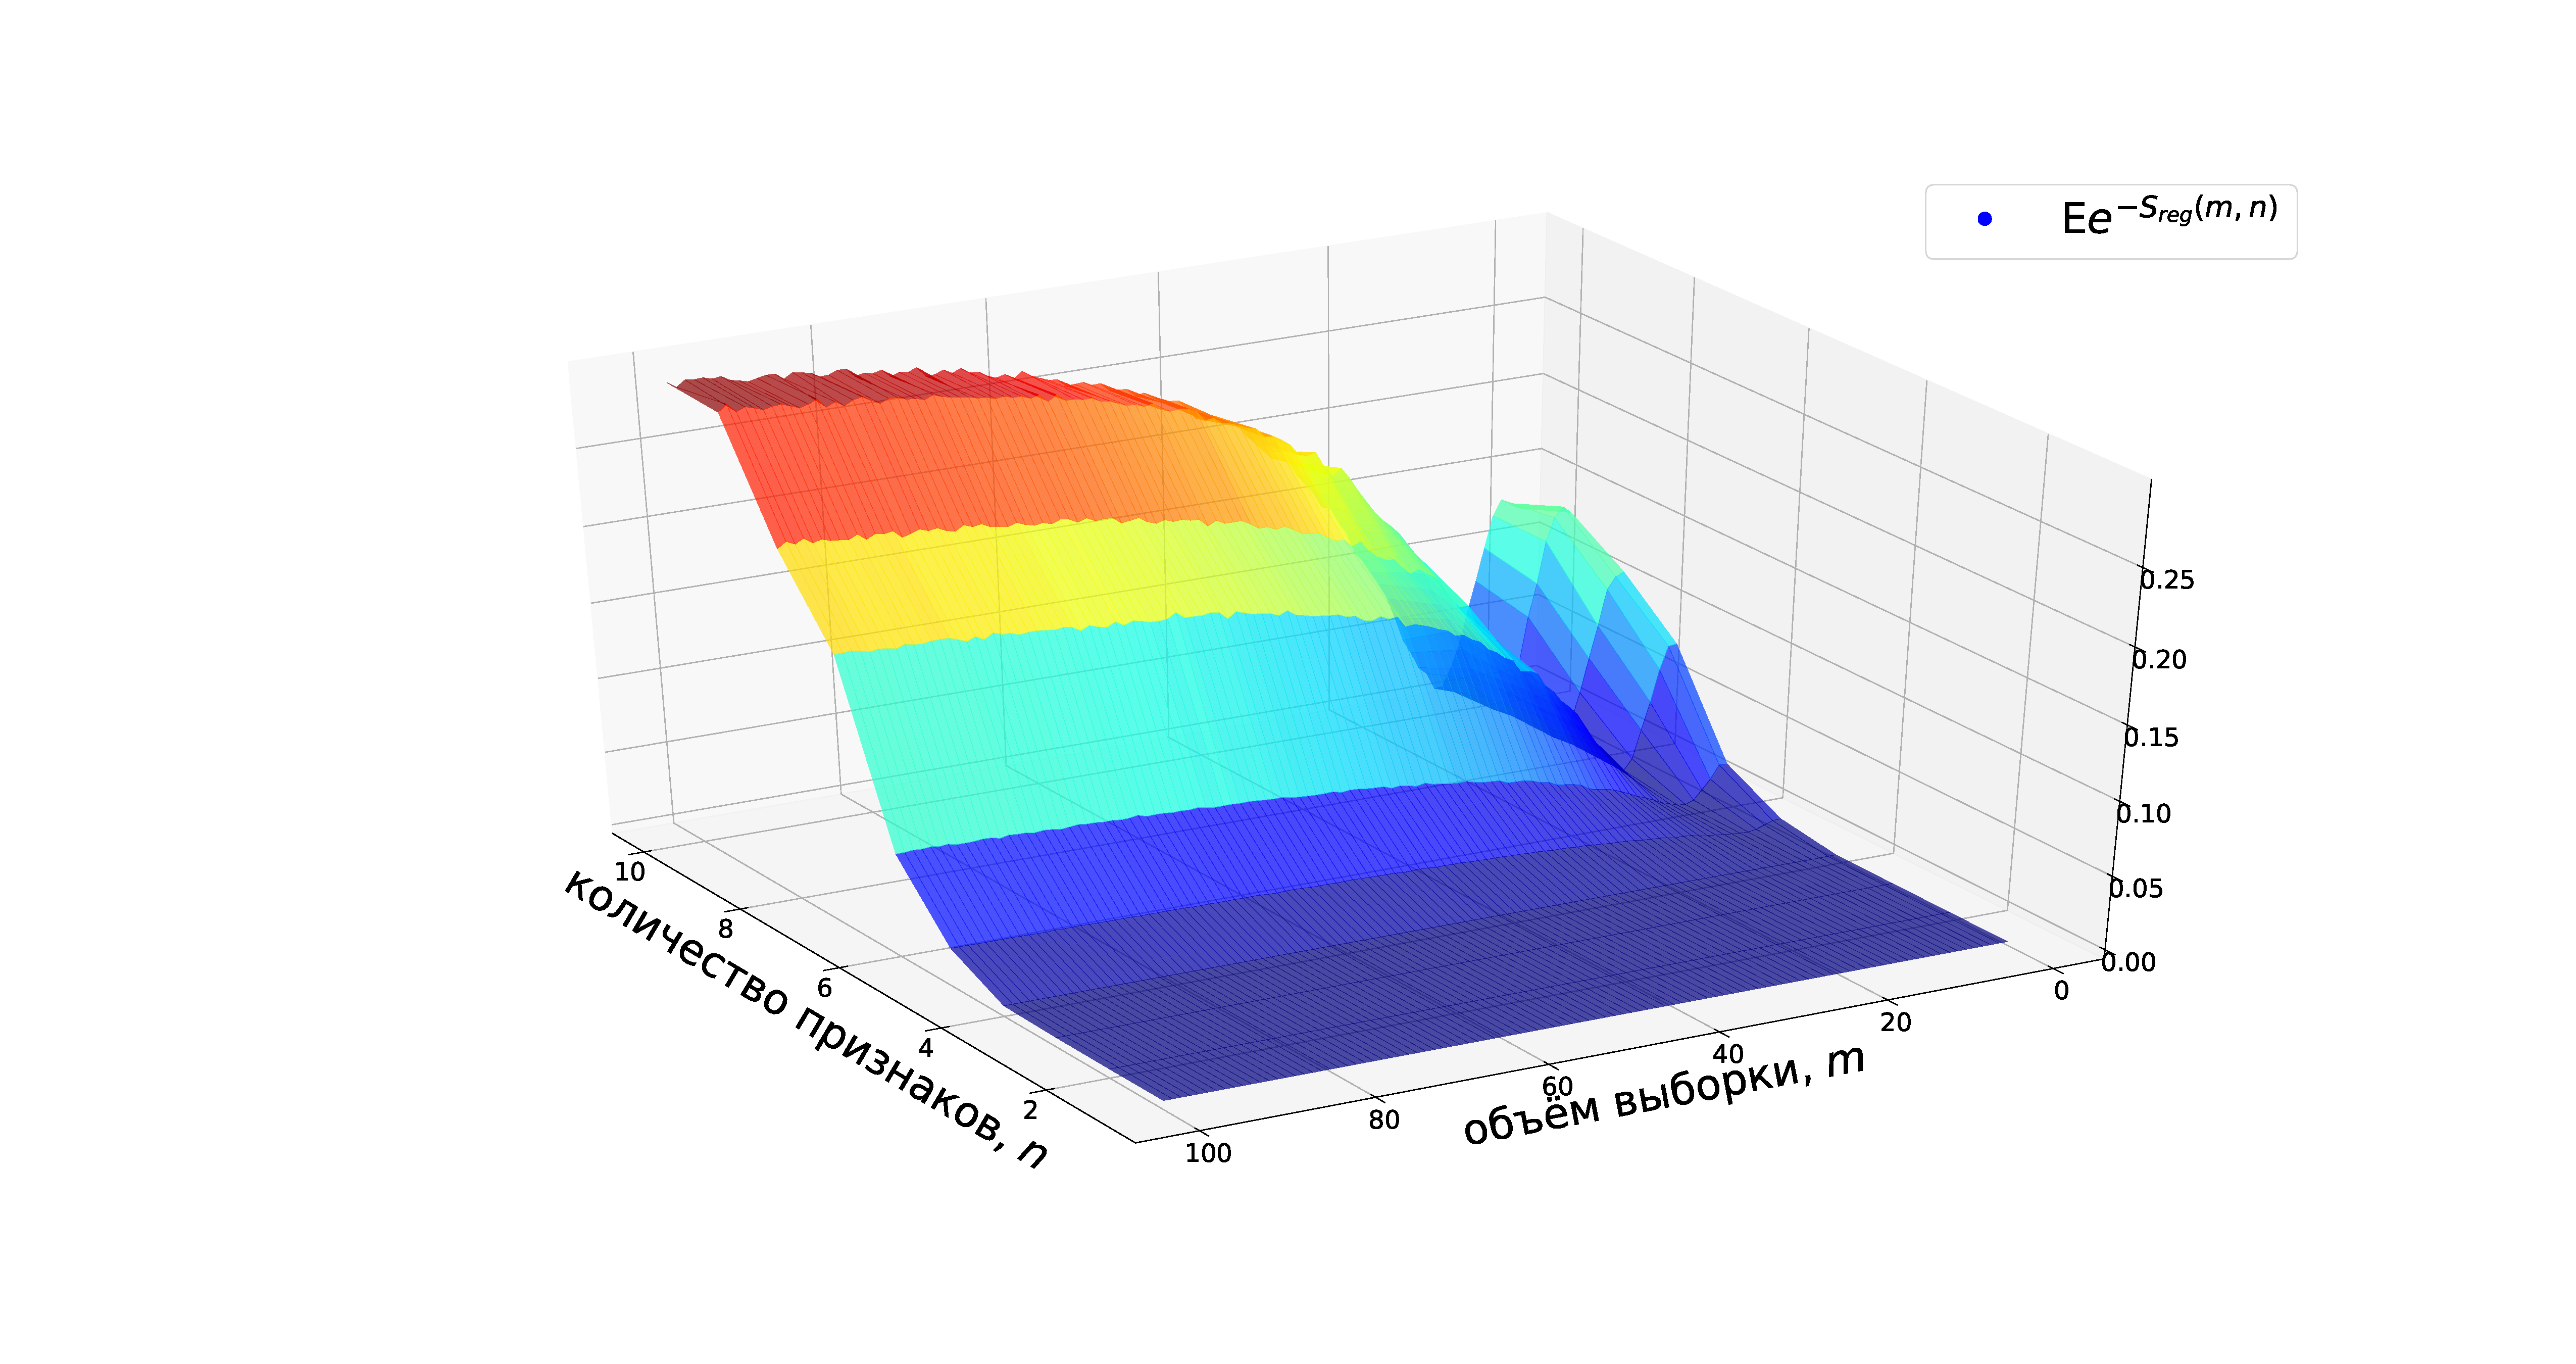
\includegraphics[width=0.5\textwidth]{../data/pics/adequate_random_sample_llh.pdf}}&
\subfloat[Случайная выборка]{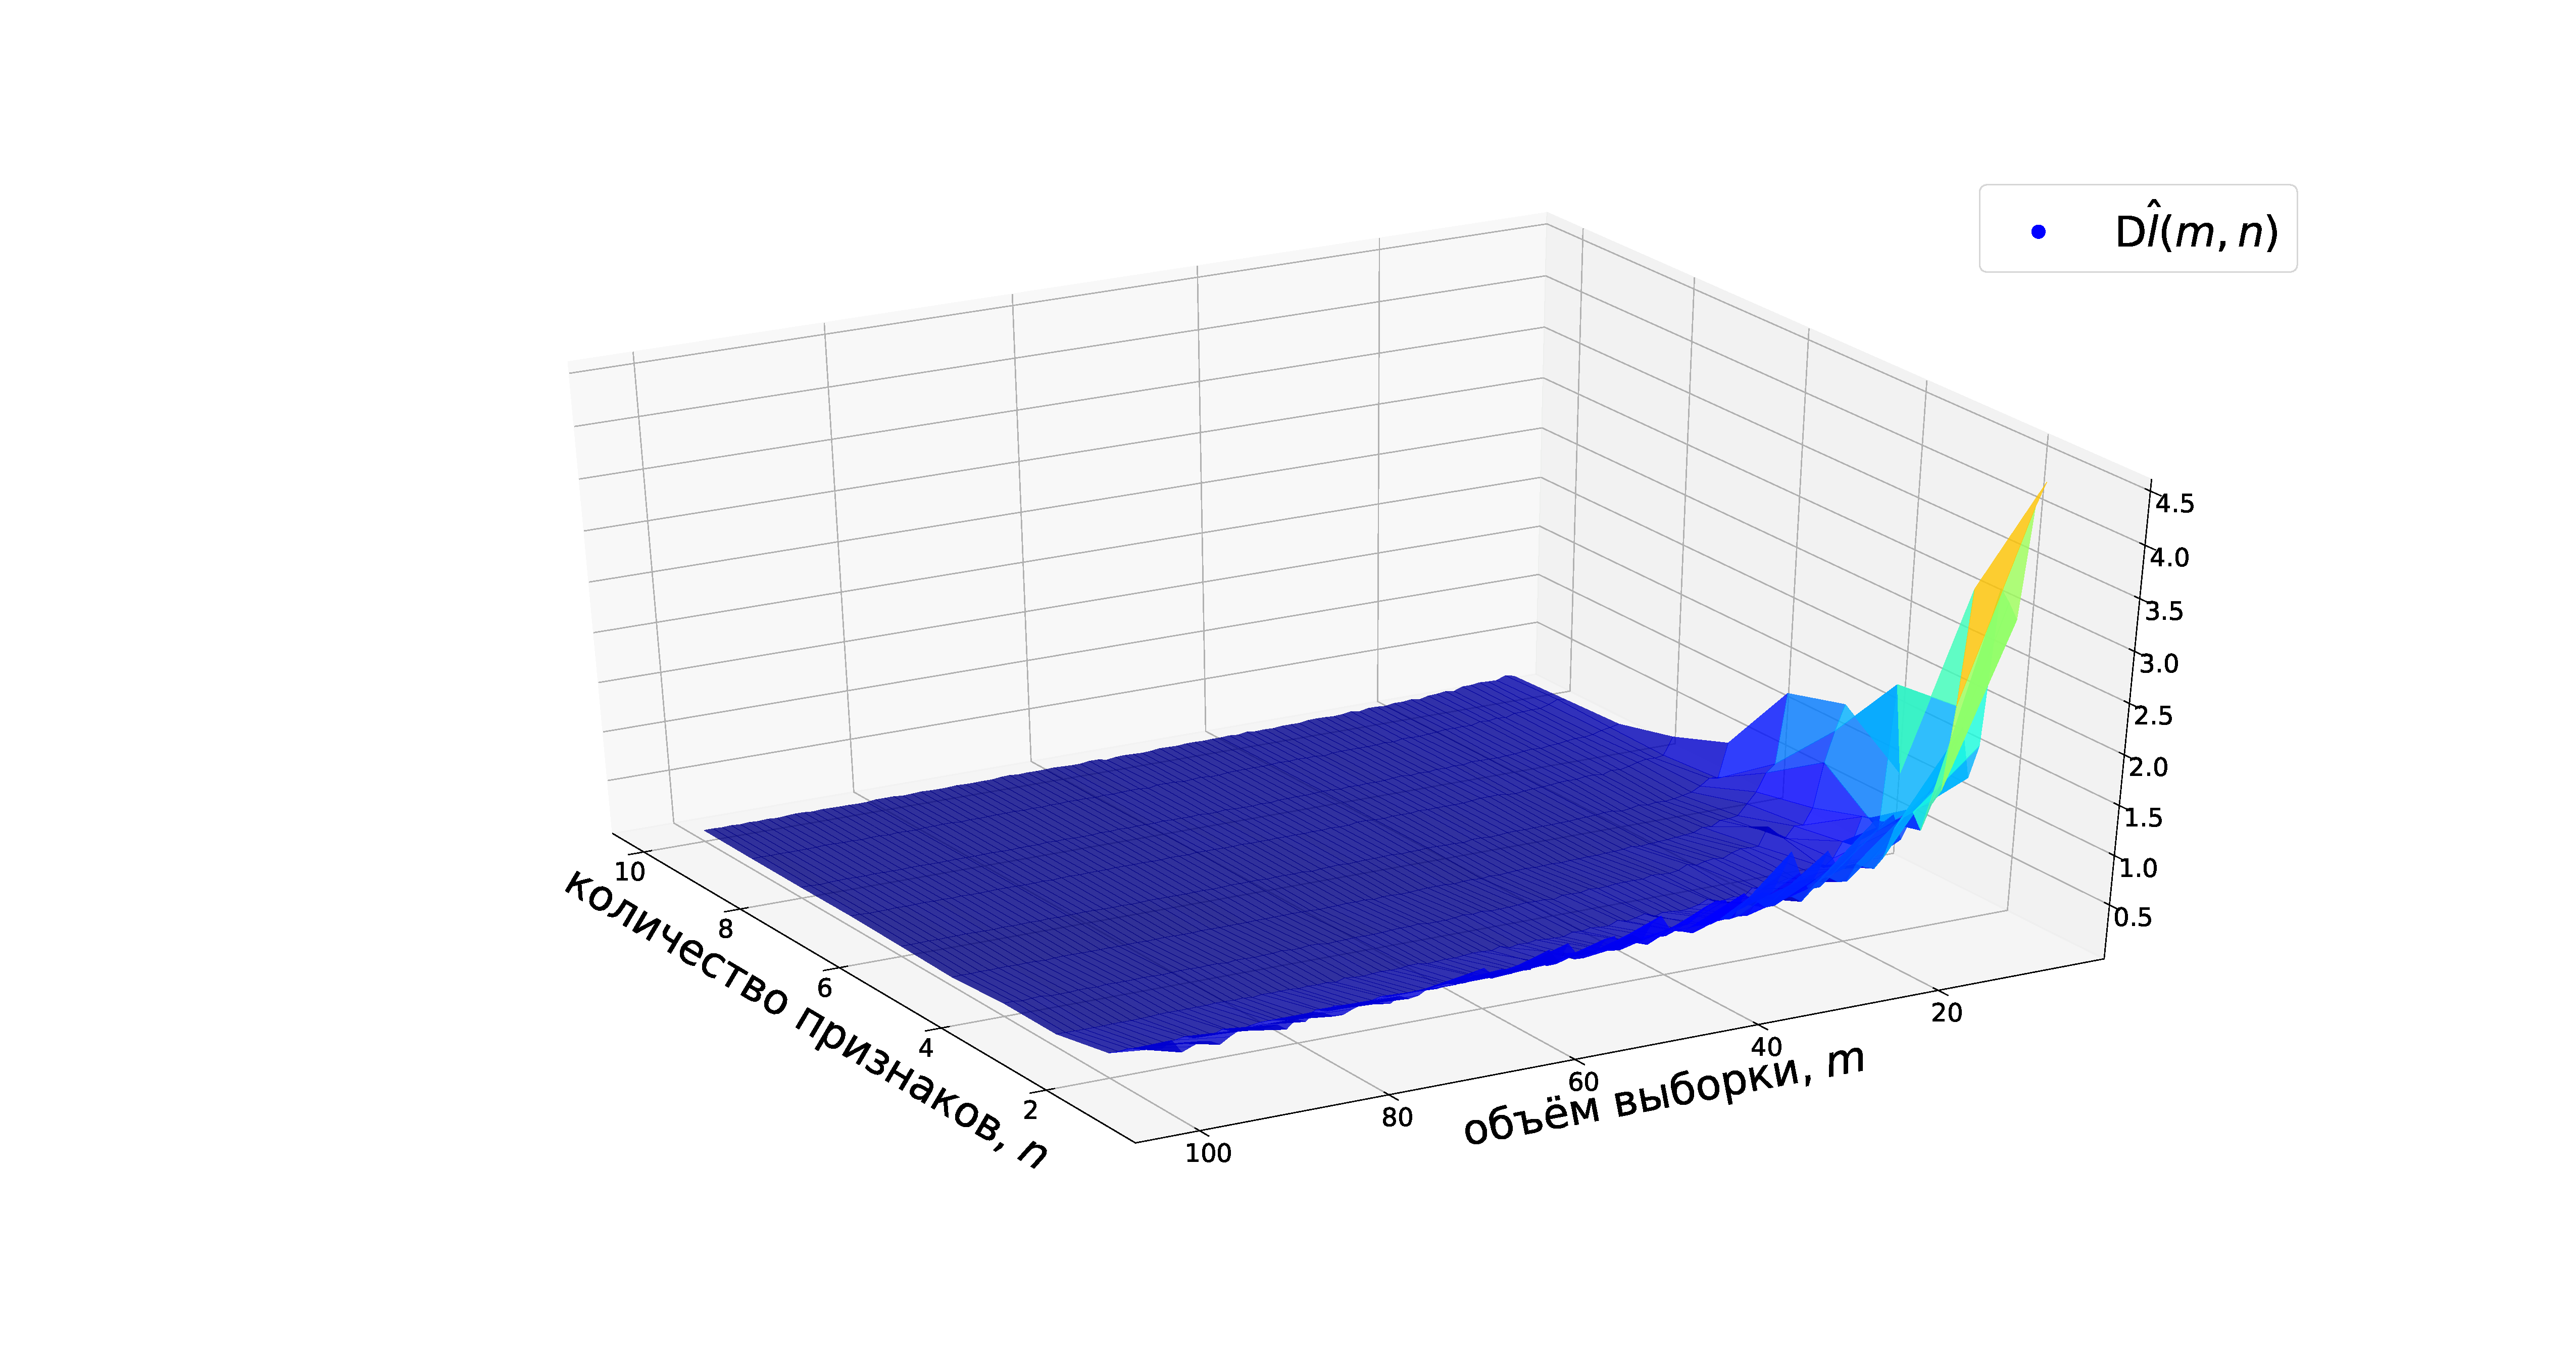
\includegraphics[width=0.5\textwidth]{../data/pics/adequate_random_sample_llh_std.pdf}}\\
\subfloat[Скоррелированная выборка]{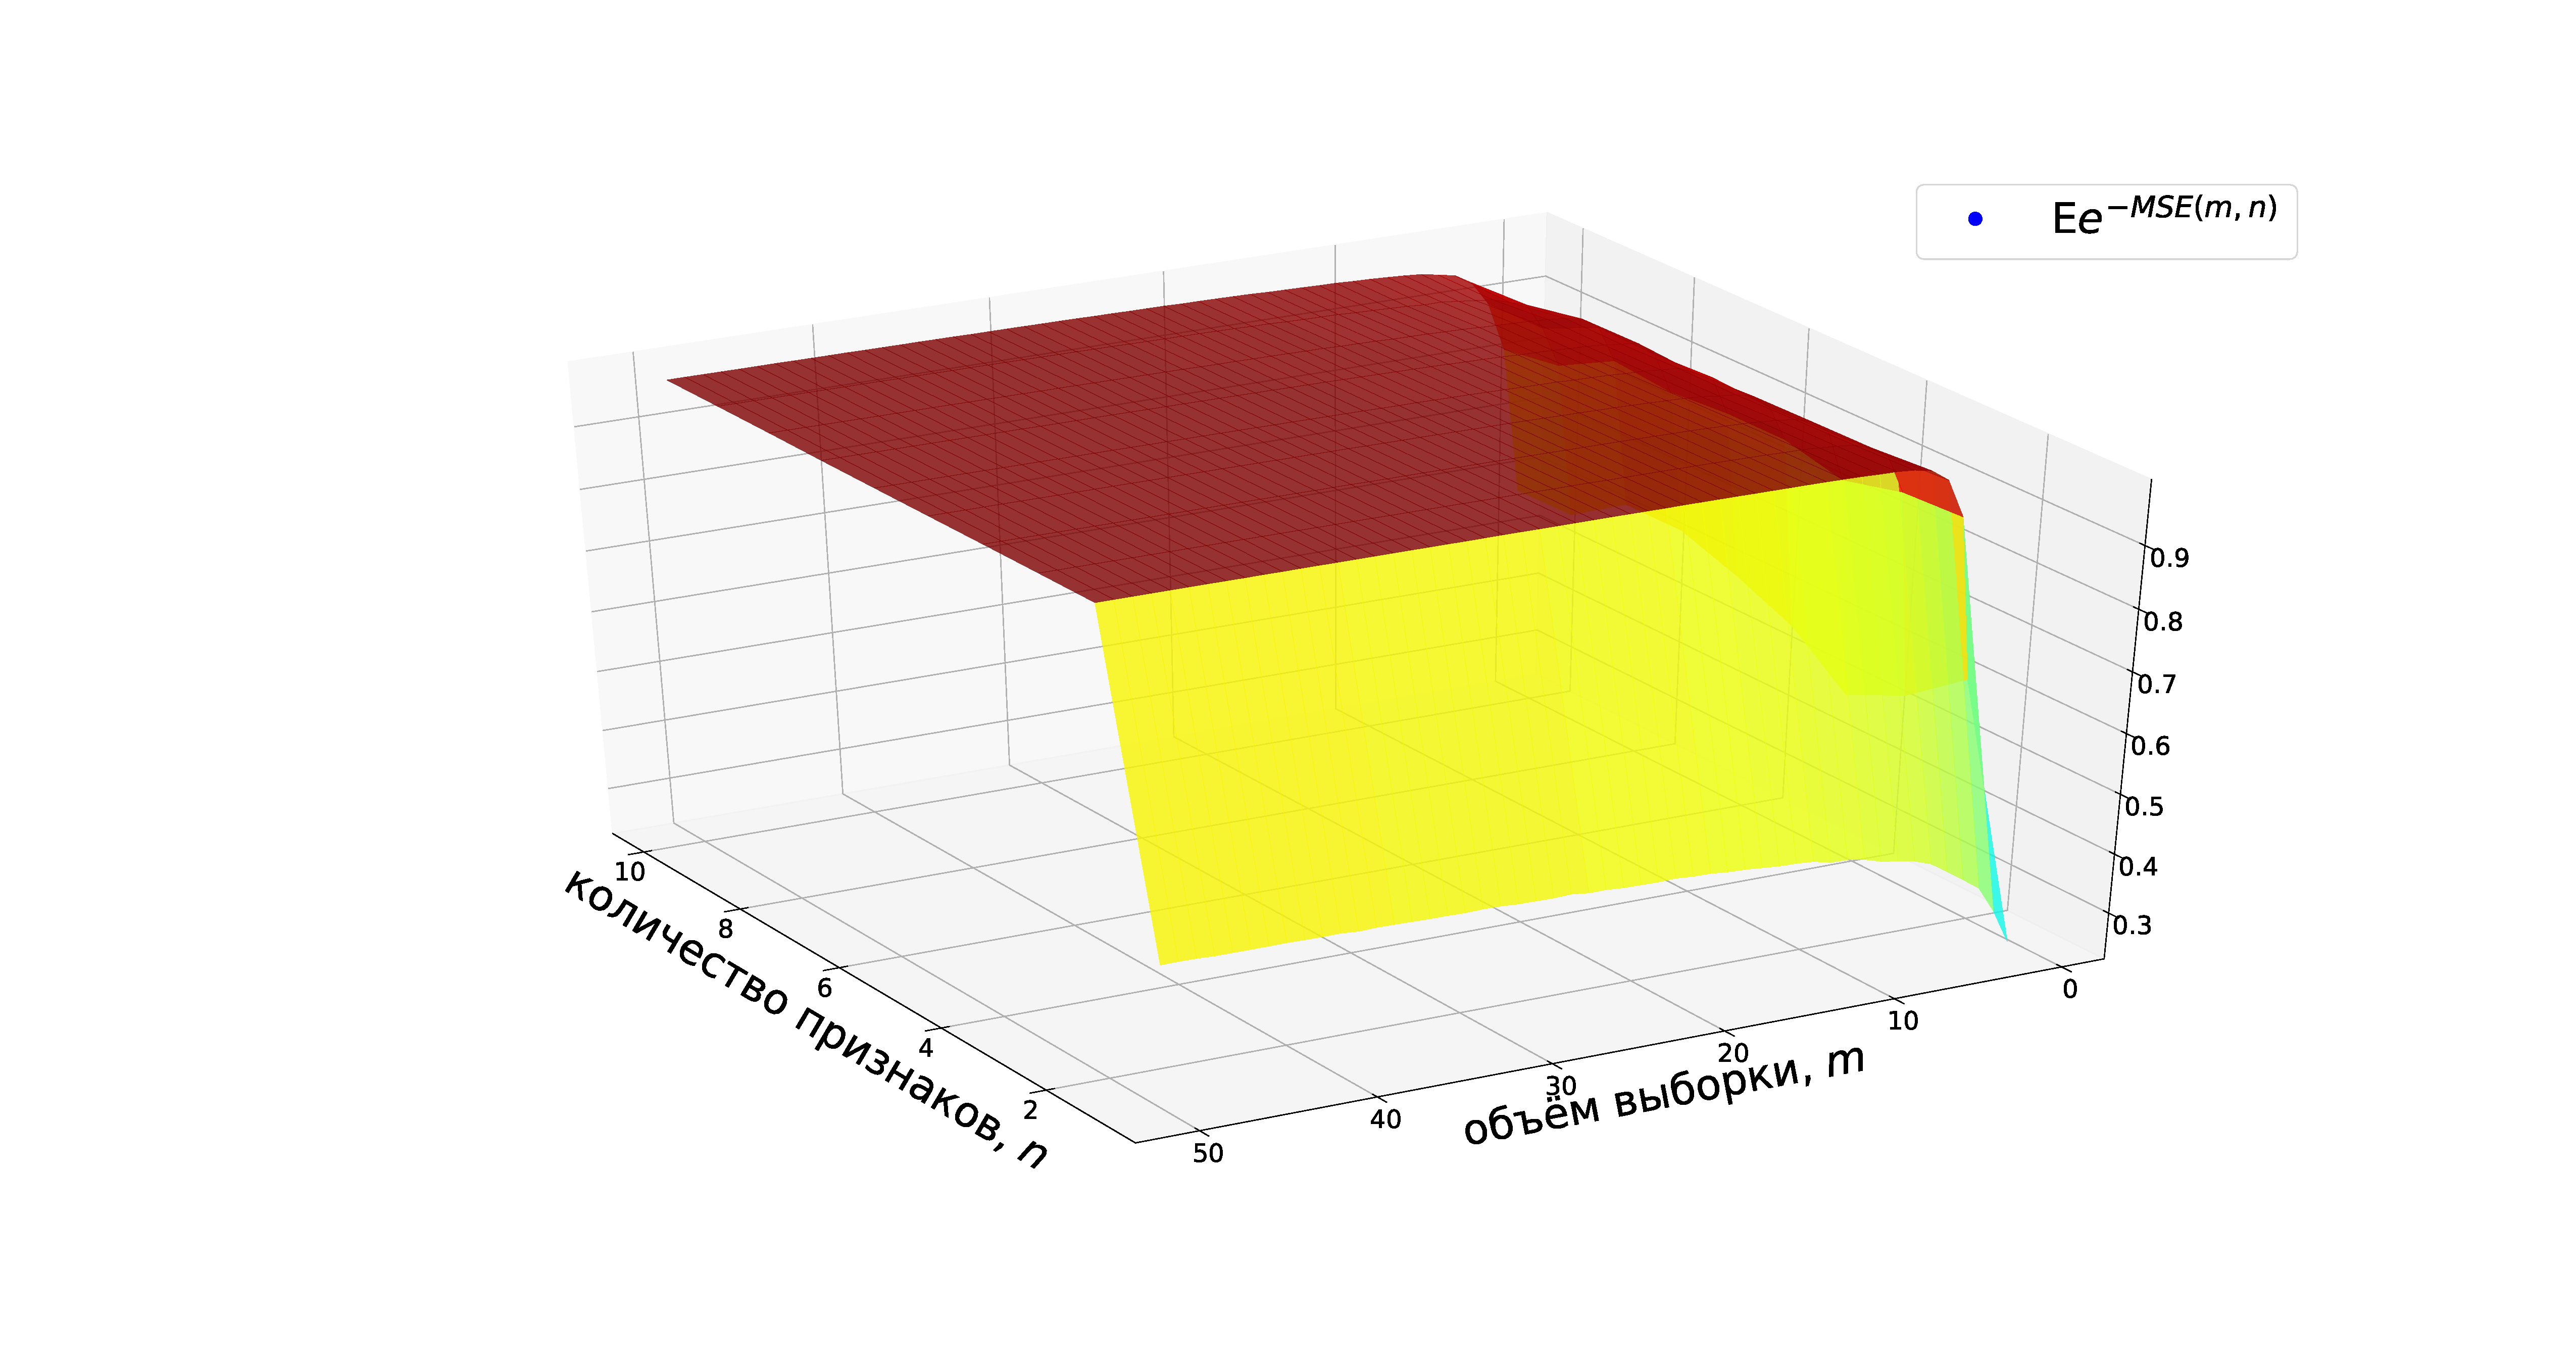
\includegraphics[width=0.5\textwidth]{../data/pics/adequate_correlated_sample_llh.pdf}}&
\subfloat[Скоррелированная выборка]{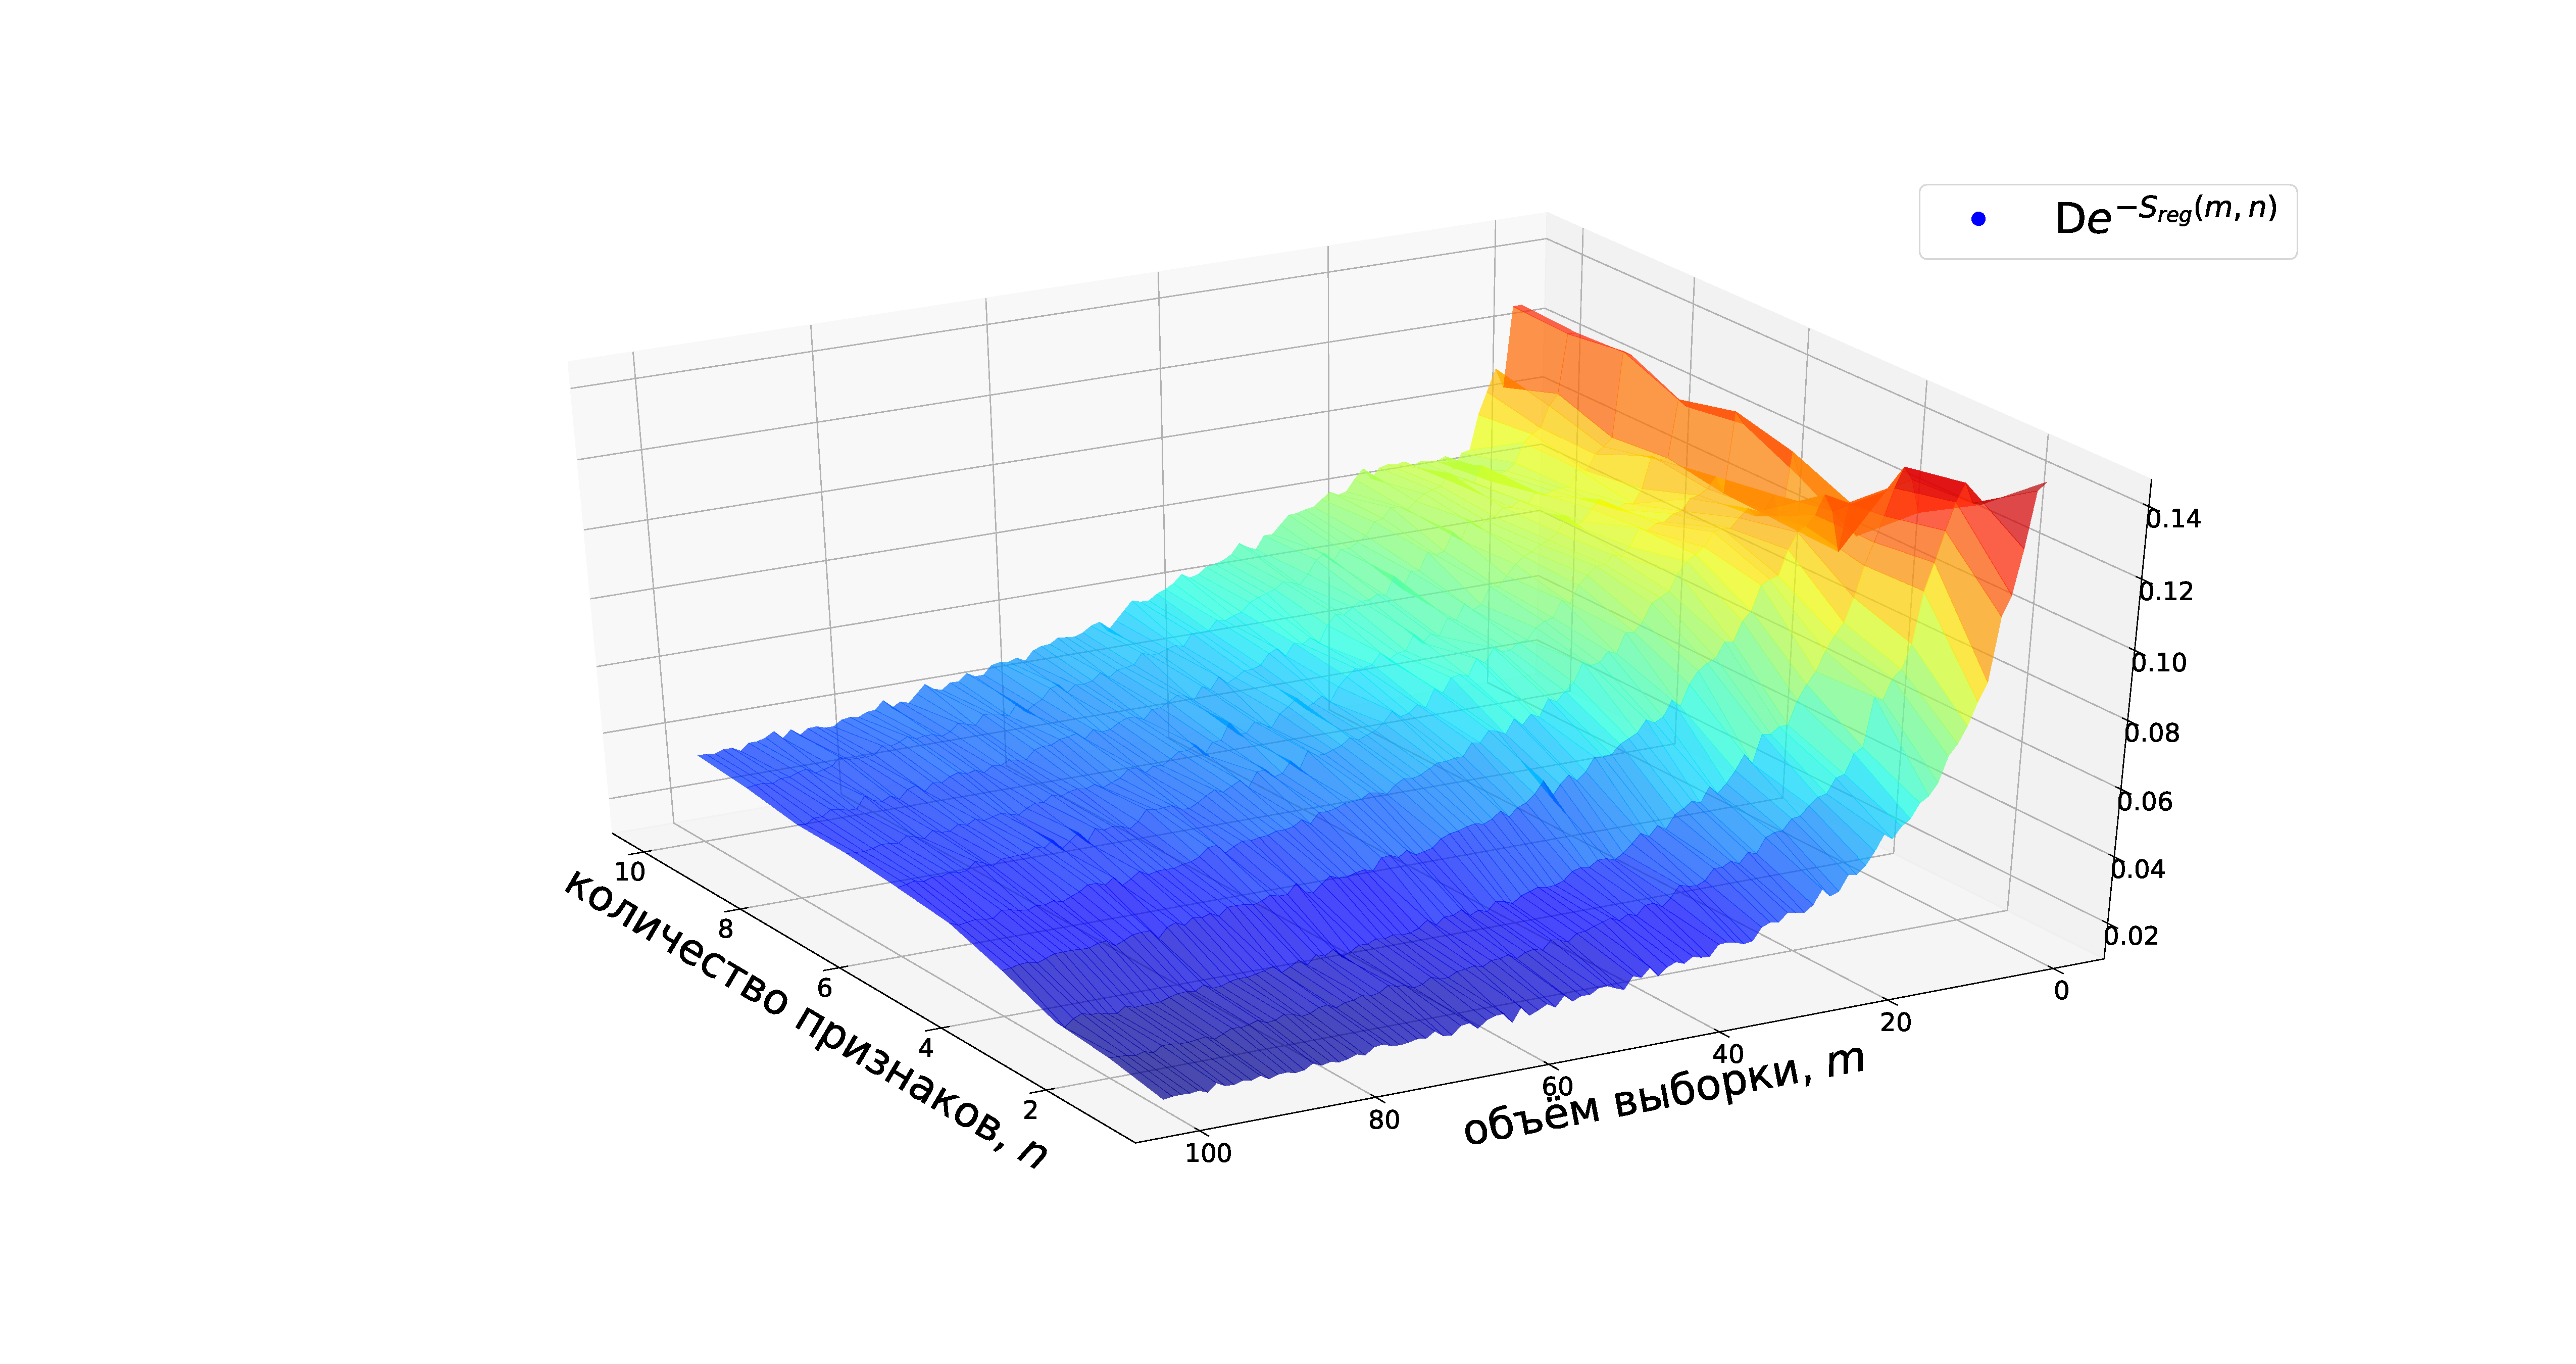
\includegraphics[width=0.5\textwidth]{../data/pics/adequate_correlated_sample_llh_std.pdf}}\\
\subfloat[Ортогональная выборка]{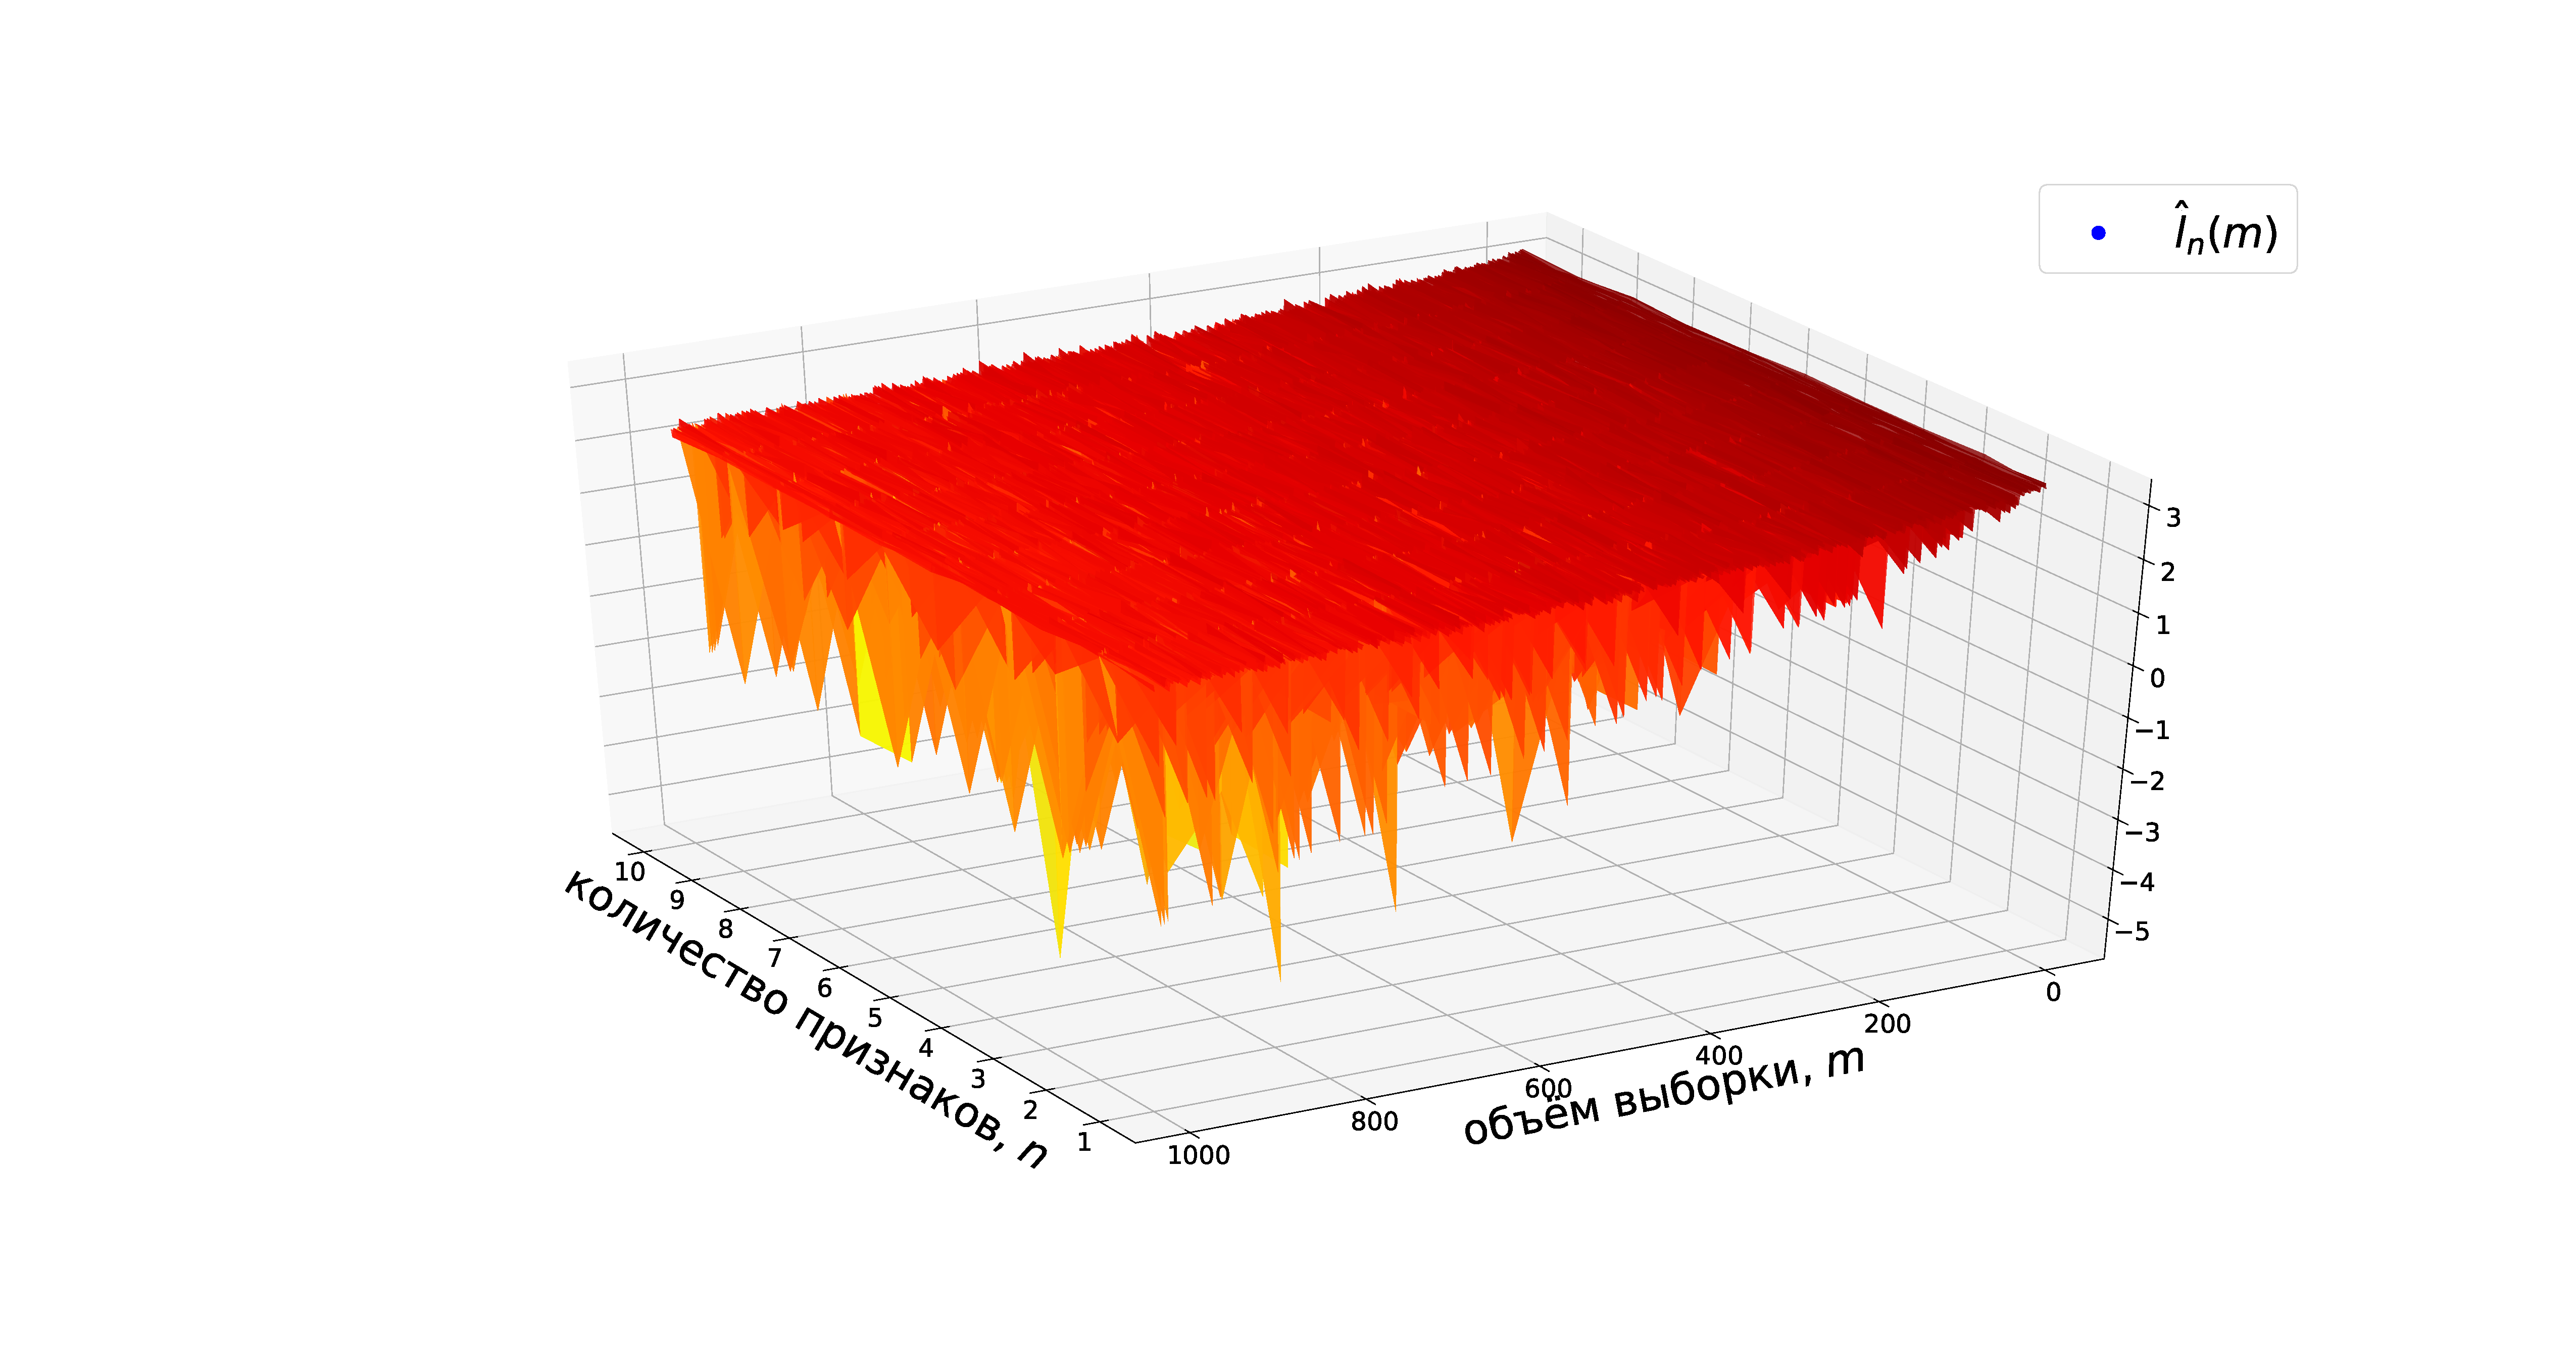
\includegraphics[width=0.5\textwidth]{../data/pics/adequate_orthogonal_sample_llh.pdf}}&
\subfloat[Ортогональная выборка]{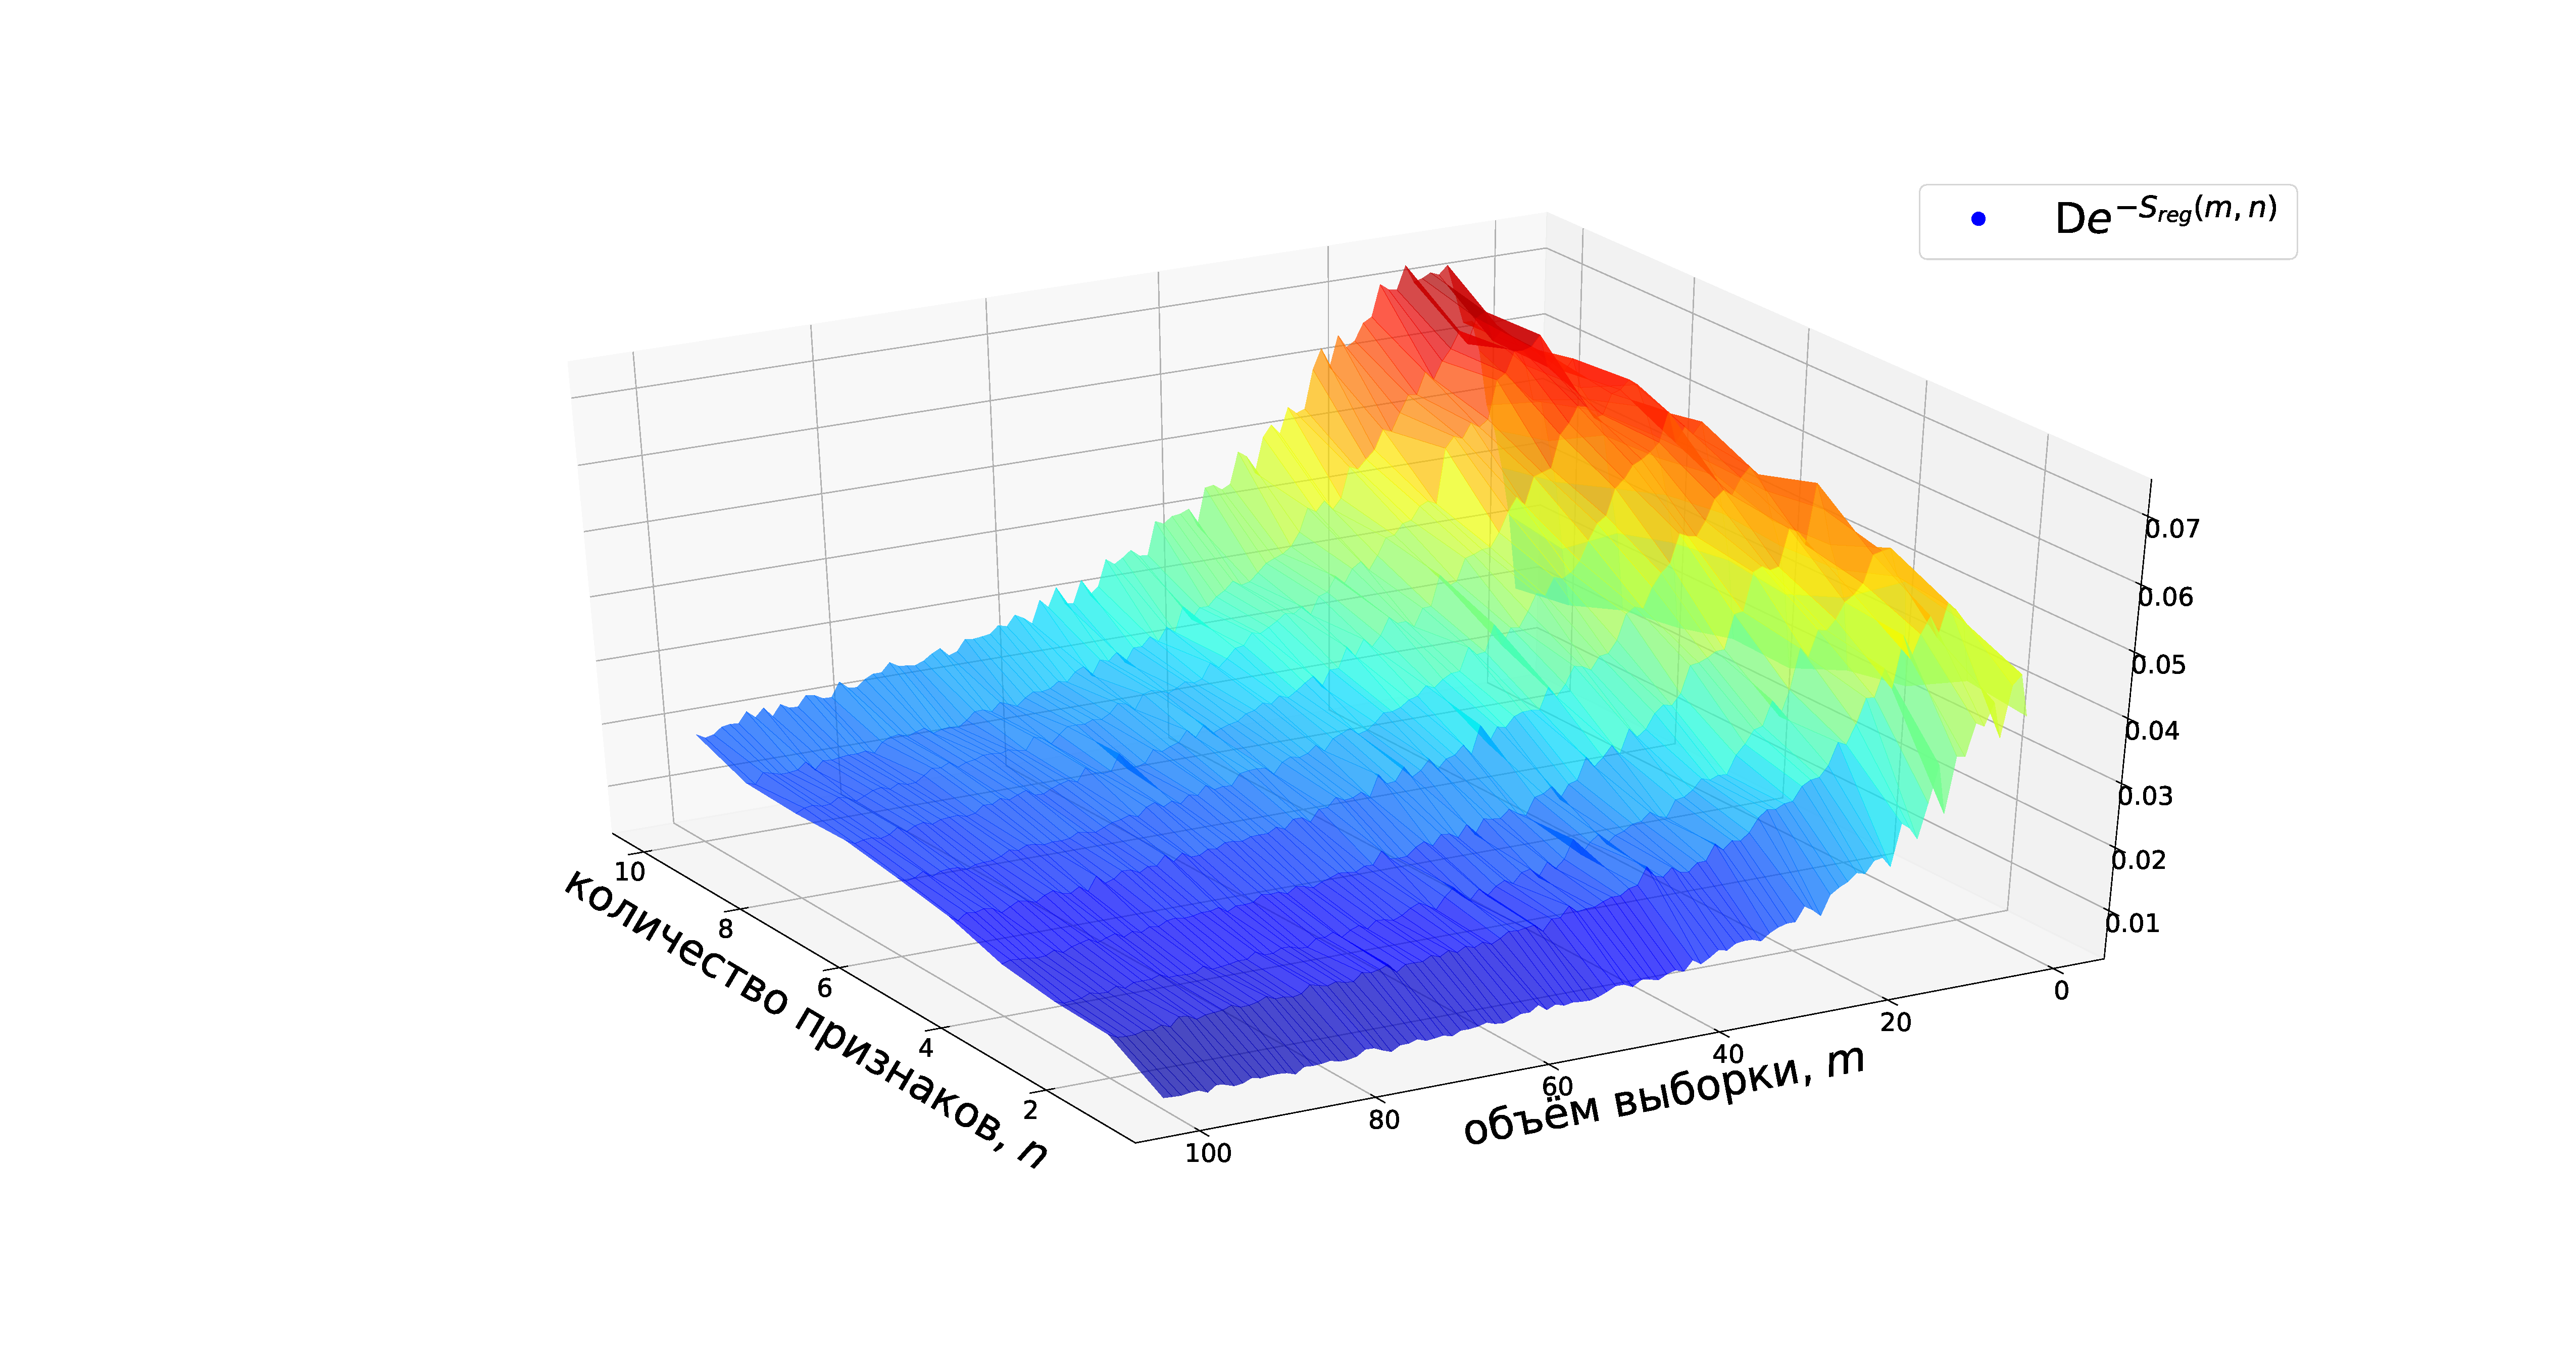
\includegraphics[width=0.5\textwidth]{../data/pics/adequate_orthogonal_sample_llh_std.pdf}}\\
\subfloat[Избыточная выборка]{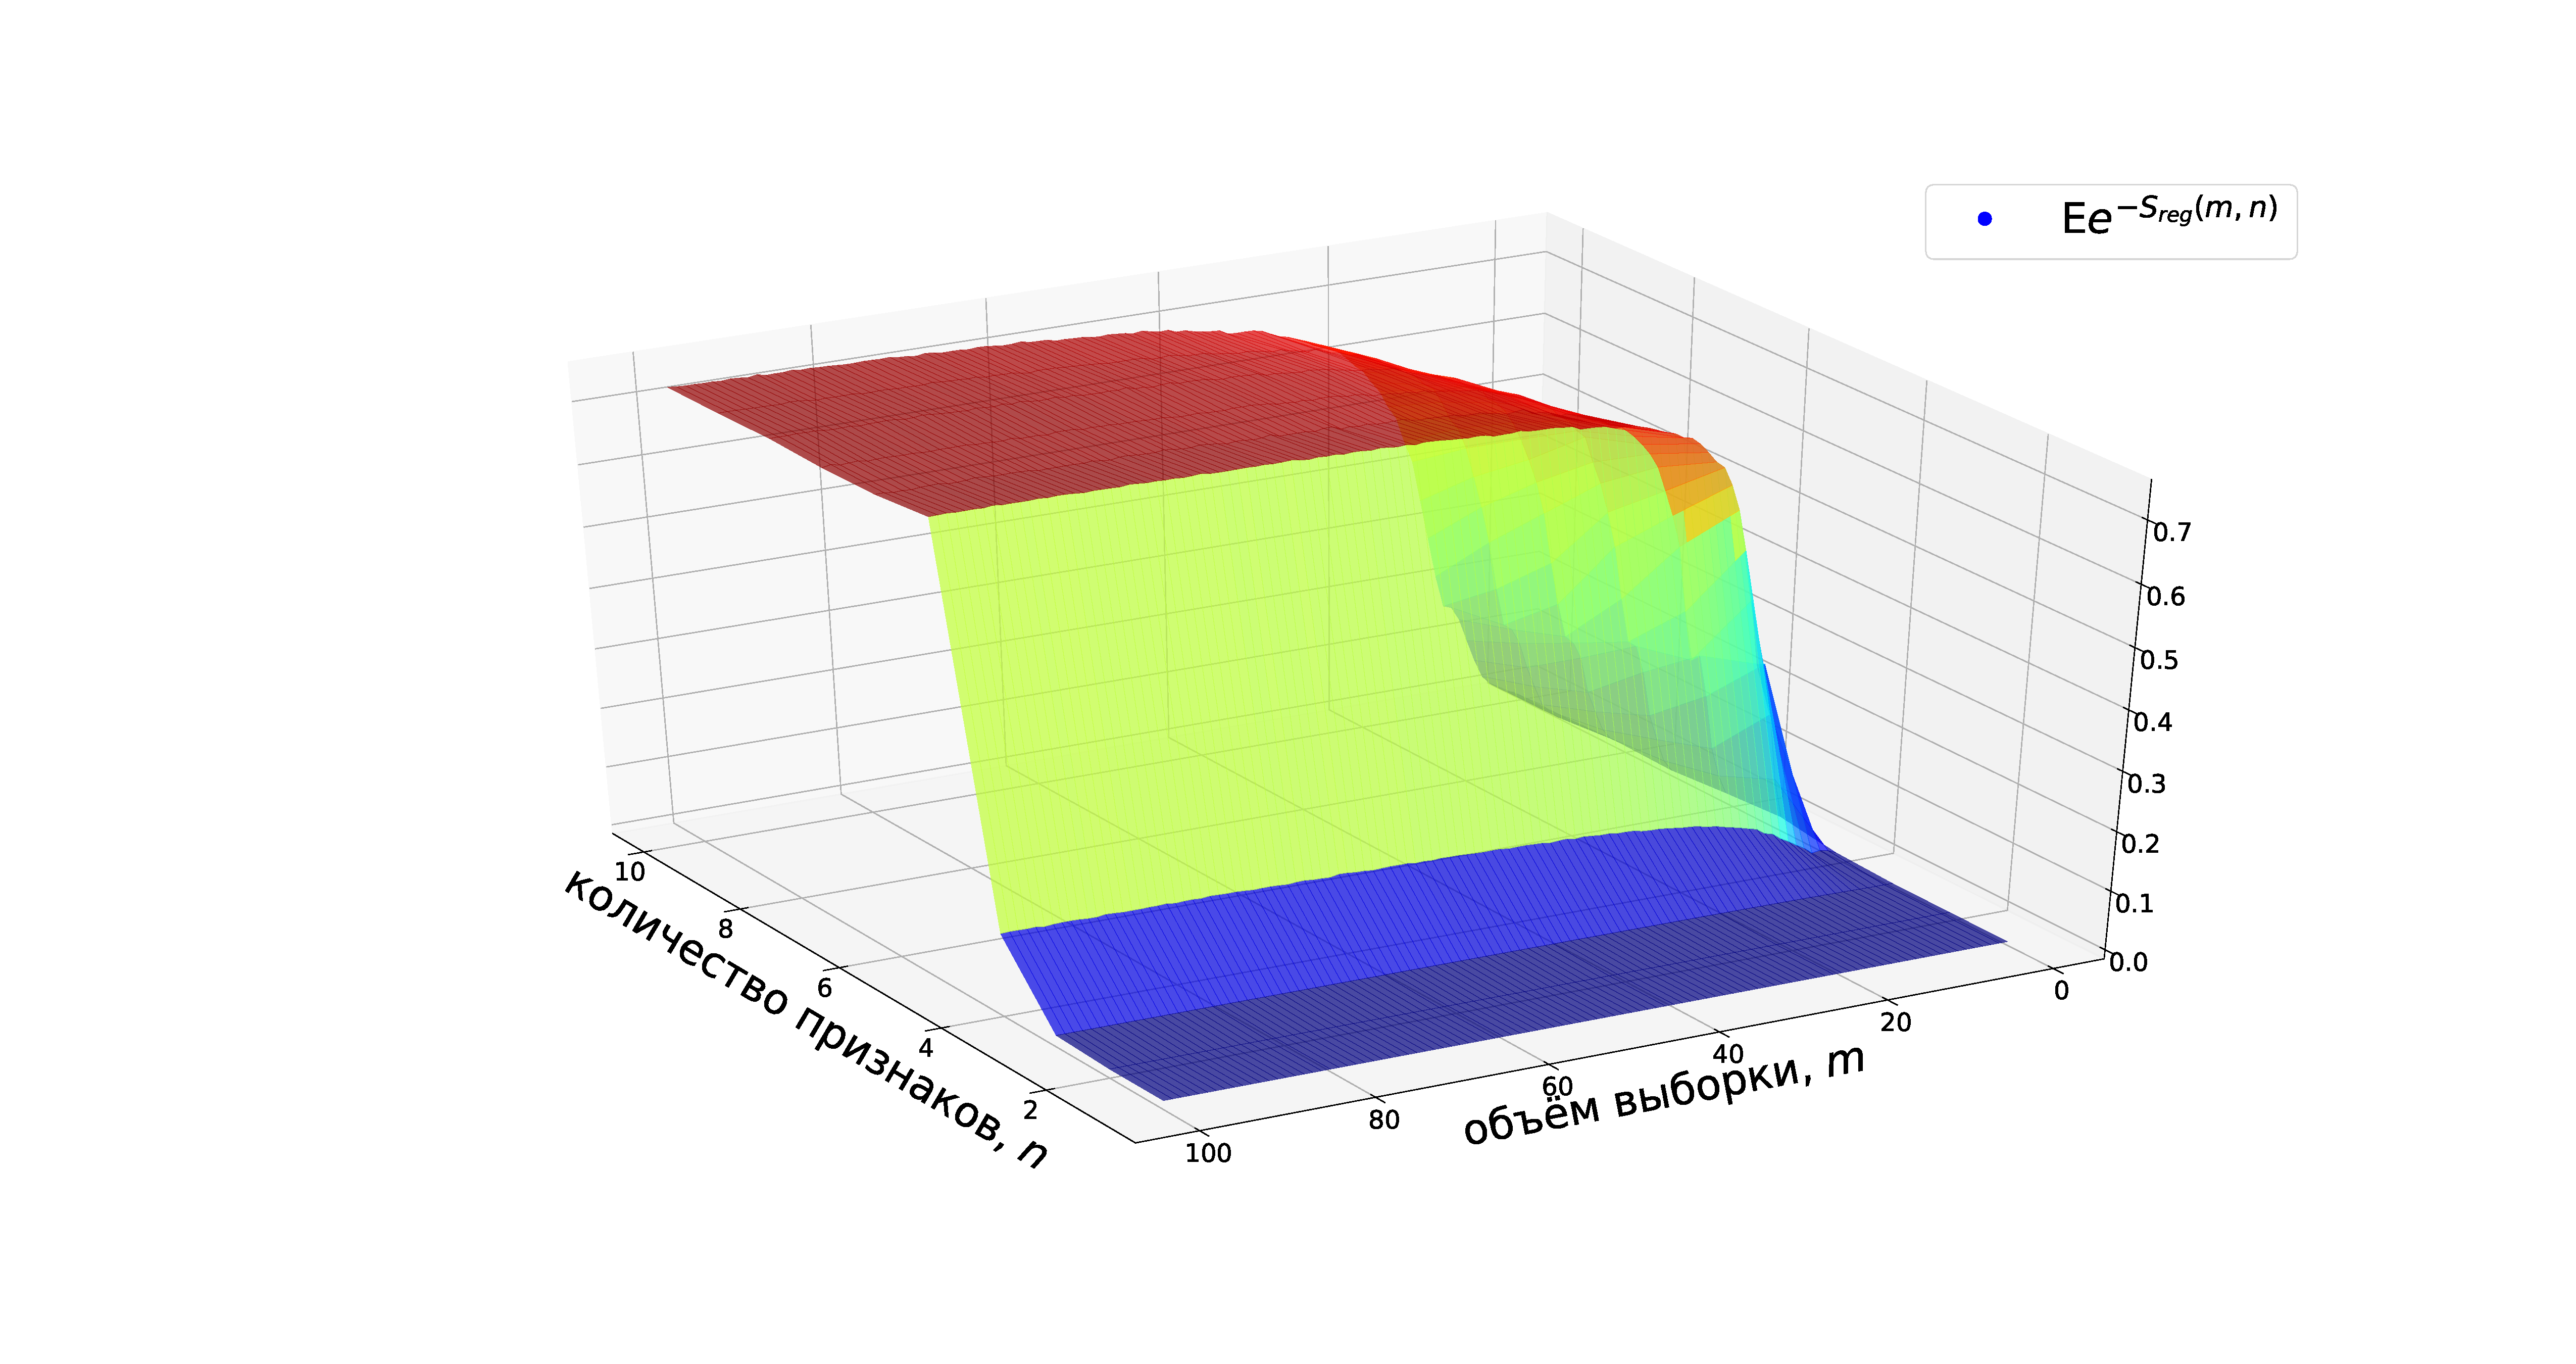
\includegraphics[width=0.5\textwidth]{../data/pics/adequate_redundant_sample_llh.pdf}}&\subfloat[Избыточная выборка]{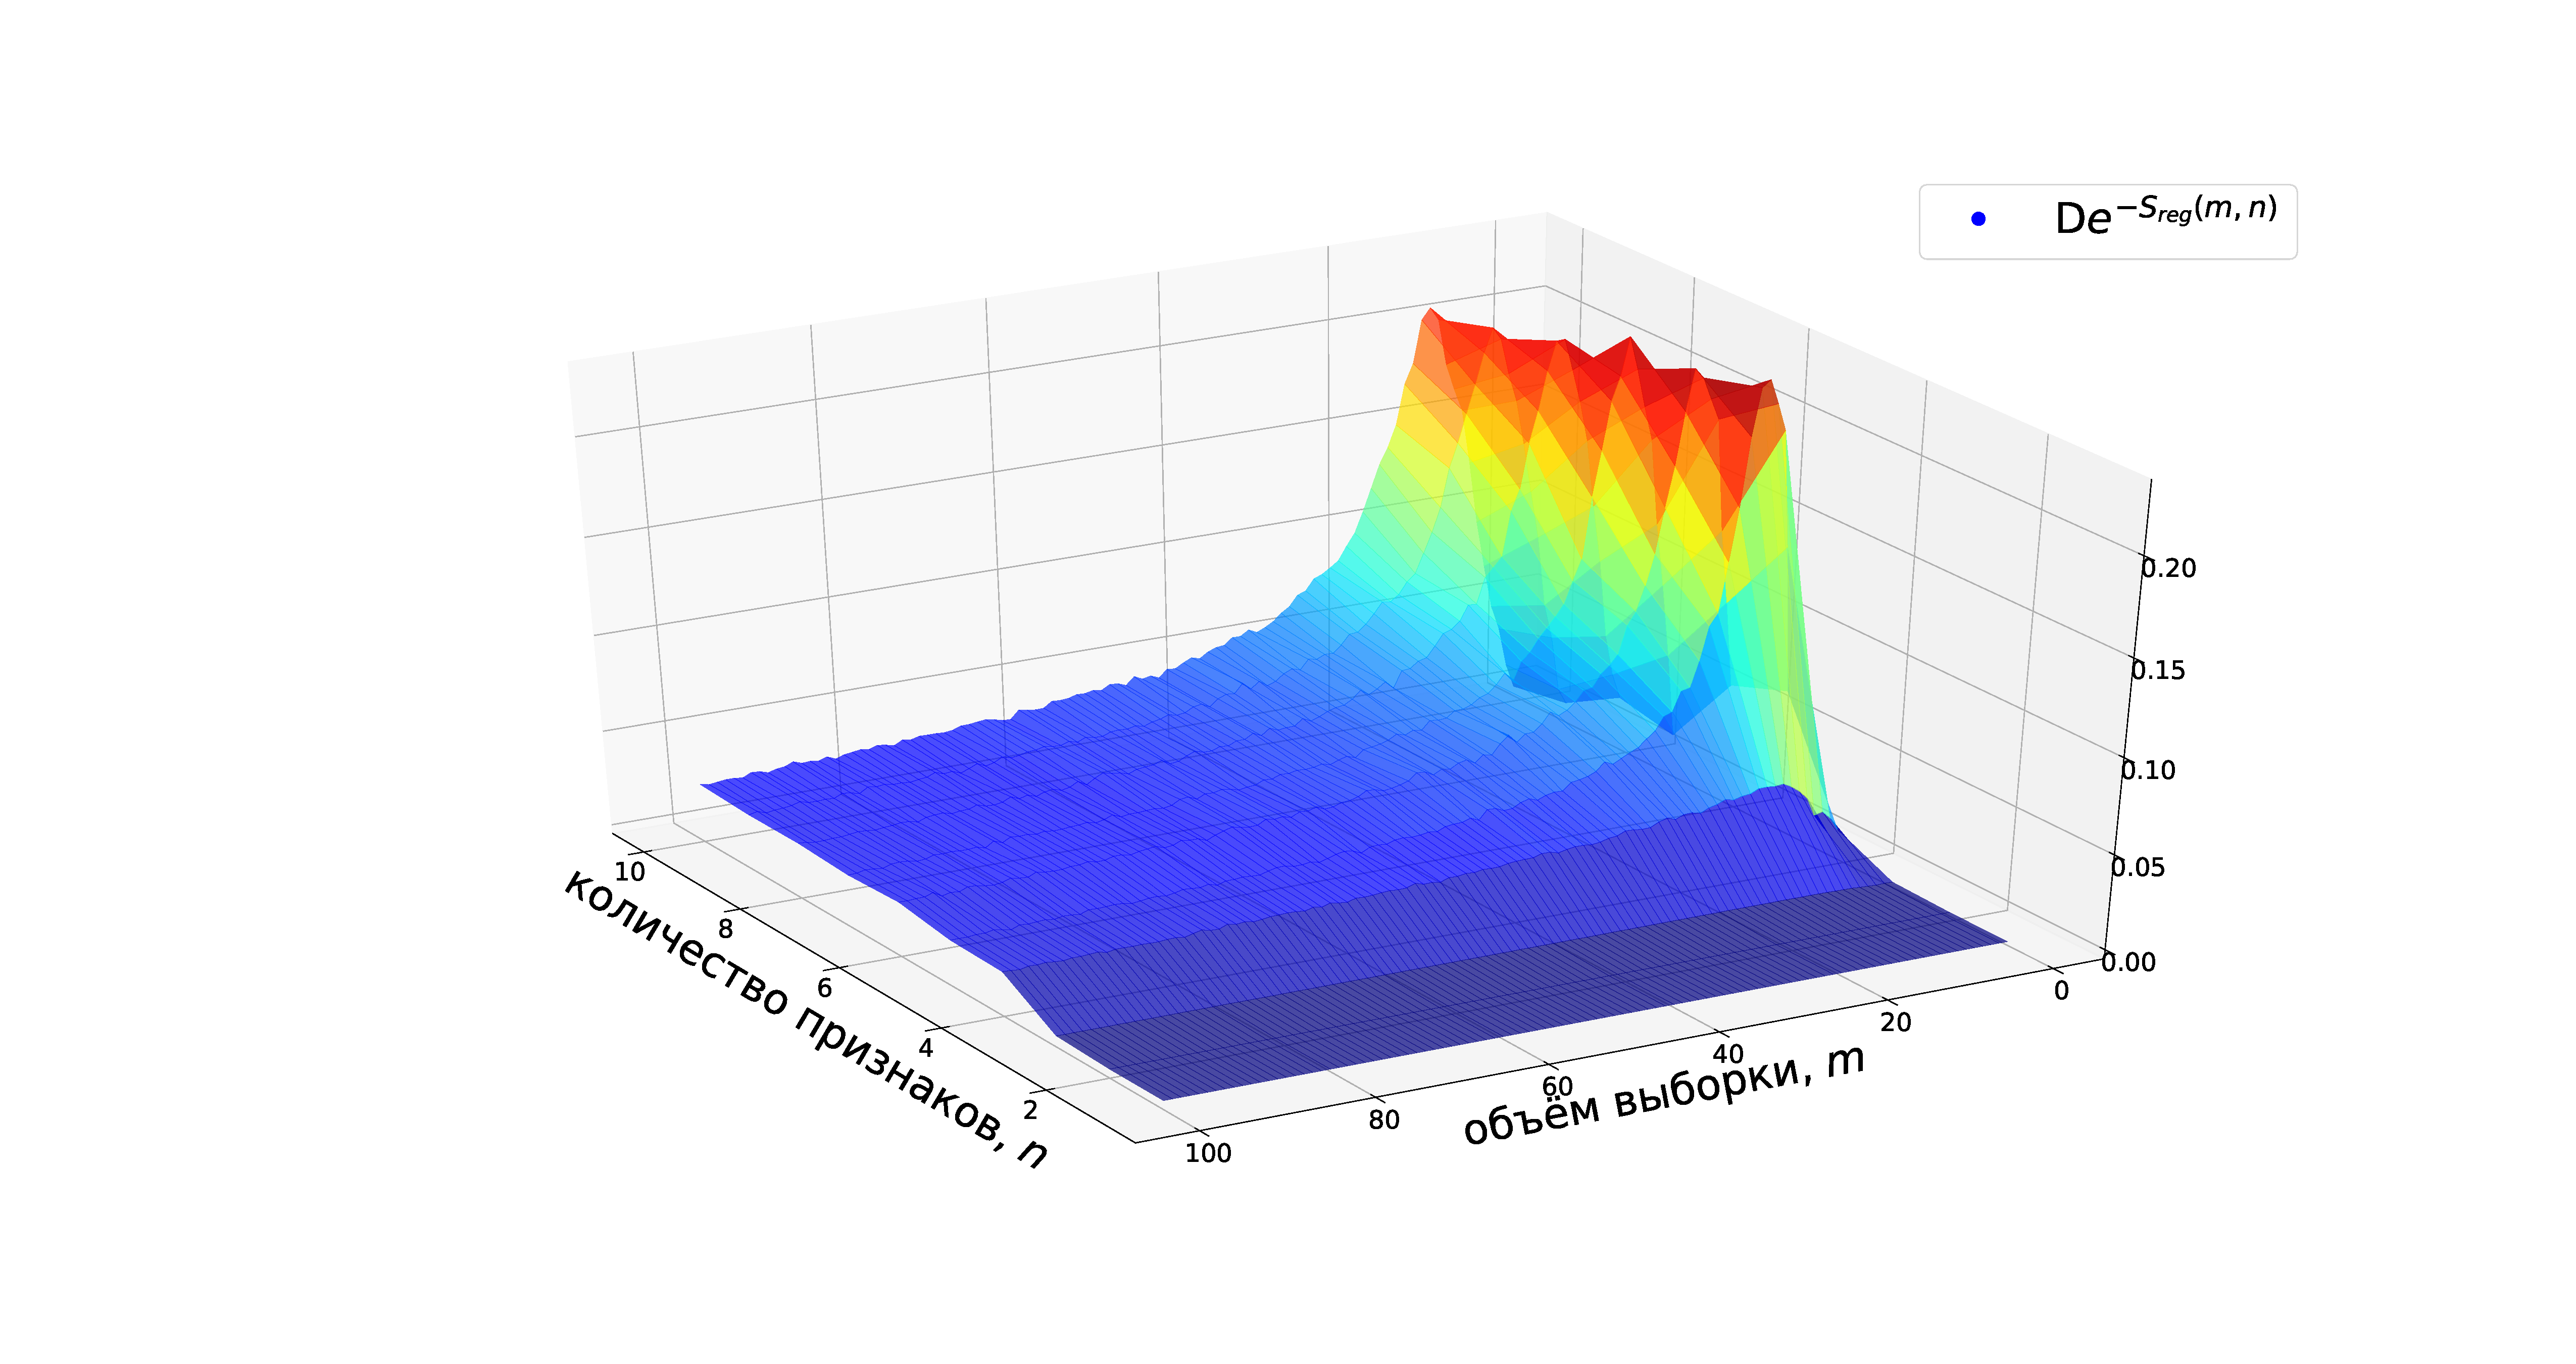
\includegraphics[width=0.5\textwidth]{../data/pics/adequate_redundant_sample_llh_std.pdf}}\\
\end{tabular}
\centering
\caption{Зависимость значения функции $e^{-S(m, n)}$ от объема выборки $m$ и количества параметров $n$ для синтетических выборок}
\label{fig1}
\end{figure}

\newpage

На рис. 2. представлены графики качества аппроксимации функции $\hat{l}(m)$, а также предсказание $\hat{m^*}$ при различных $m_0$ для разных конфигураций выборок. 

Для аппроксимации функции $\hat{l}(m)$ вариант с неполной информацией дает большую ошибку, чем вариант с полной информацией, и это ожидаемый результат. Чем меньше информации, тем хуже качество предсказания. 

При $m_0 \rightarrow m$ аппроксимация в варианте с неполной информацией стремится к аппроксимации в варианте с полной информацией, поэтому при больших $m_0$ предсказания $\hat{m^*}$ для этих двух вариантов практически совпадают.

Для случайной и избыточной выборок получилось построить адекватное предсказание при $m_0 < m^*$.

\newpage

\begin{figure}[h!t]\center
\centering\begin{tabular}{@{}c@{ }c@{ }c@{}}
\textbf{Аппроксимация $e^{-S(m, n)}$} & \textbf{Предсказание $m^*$}\\
\subfloat[Случайная выборка]{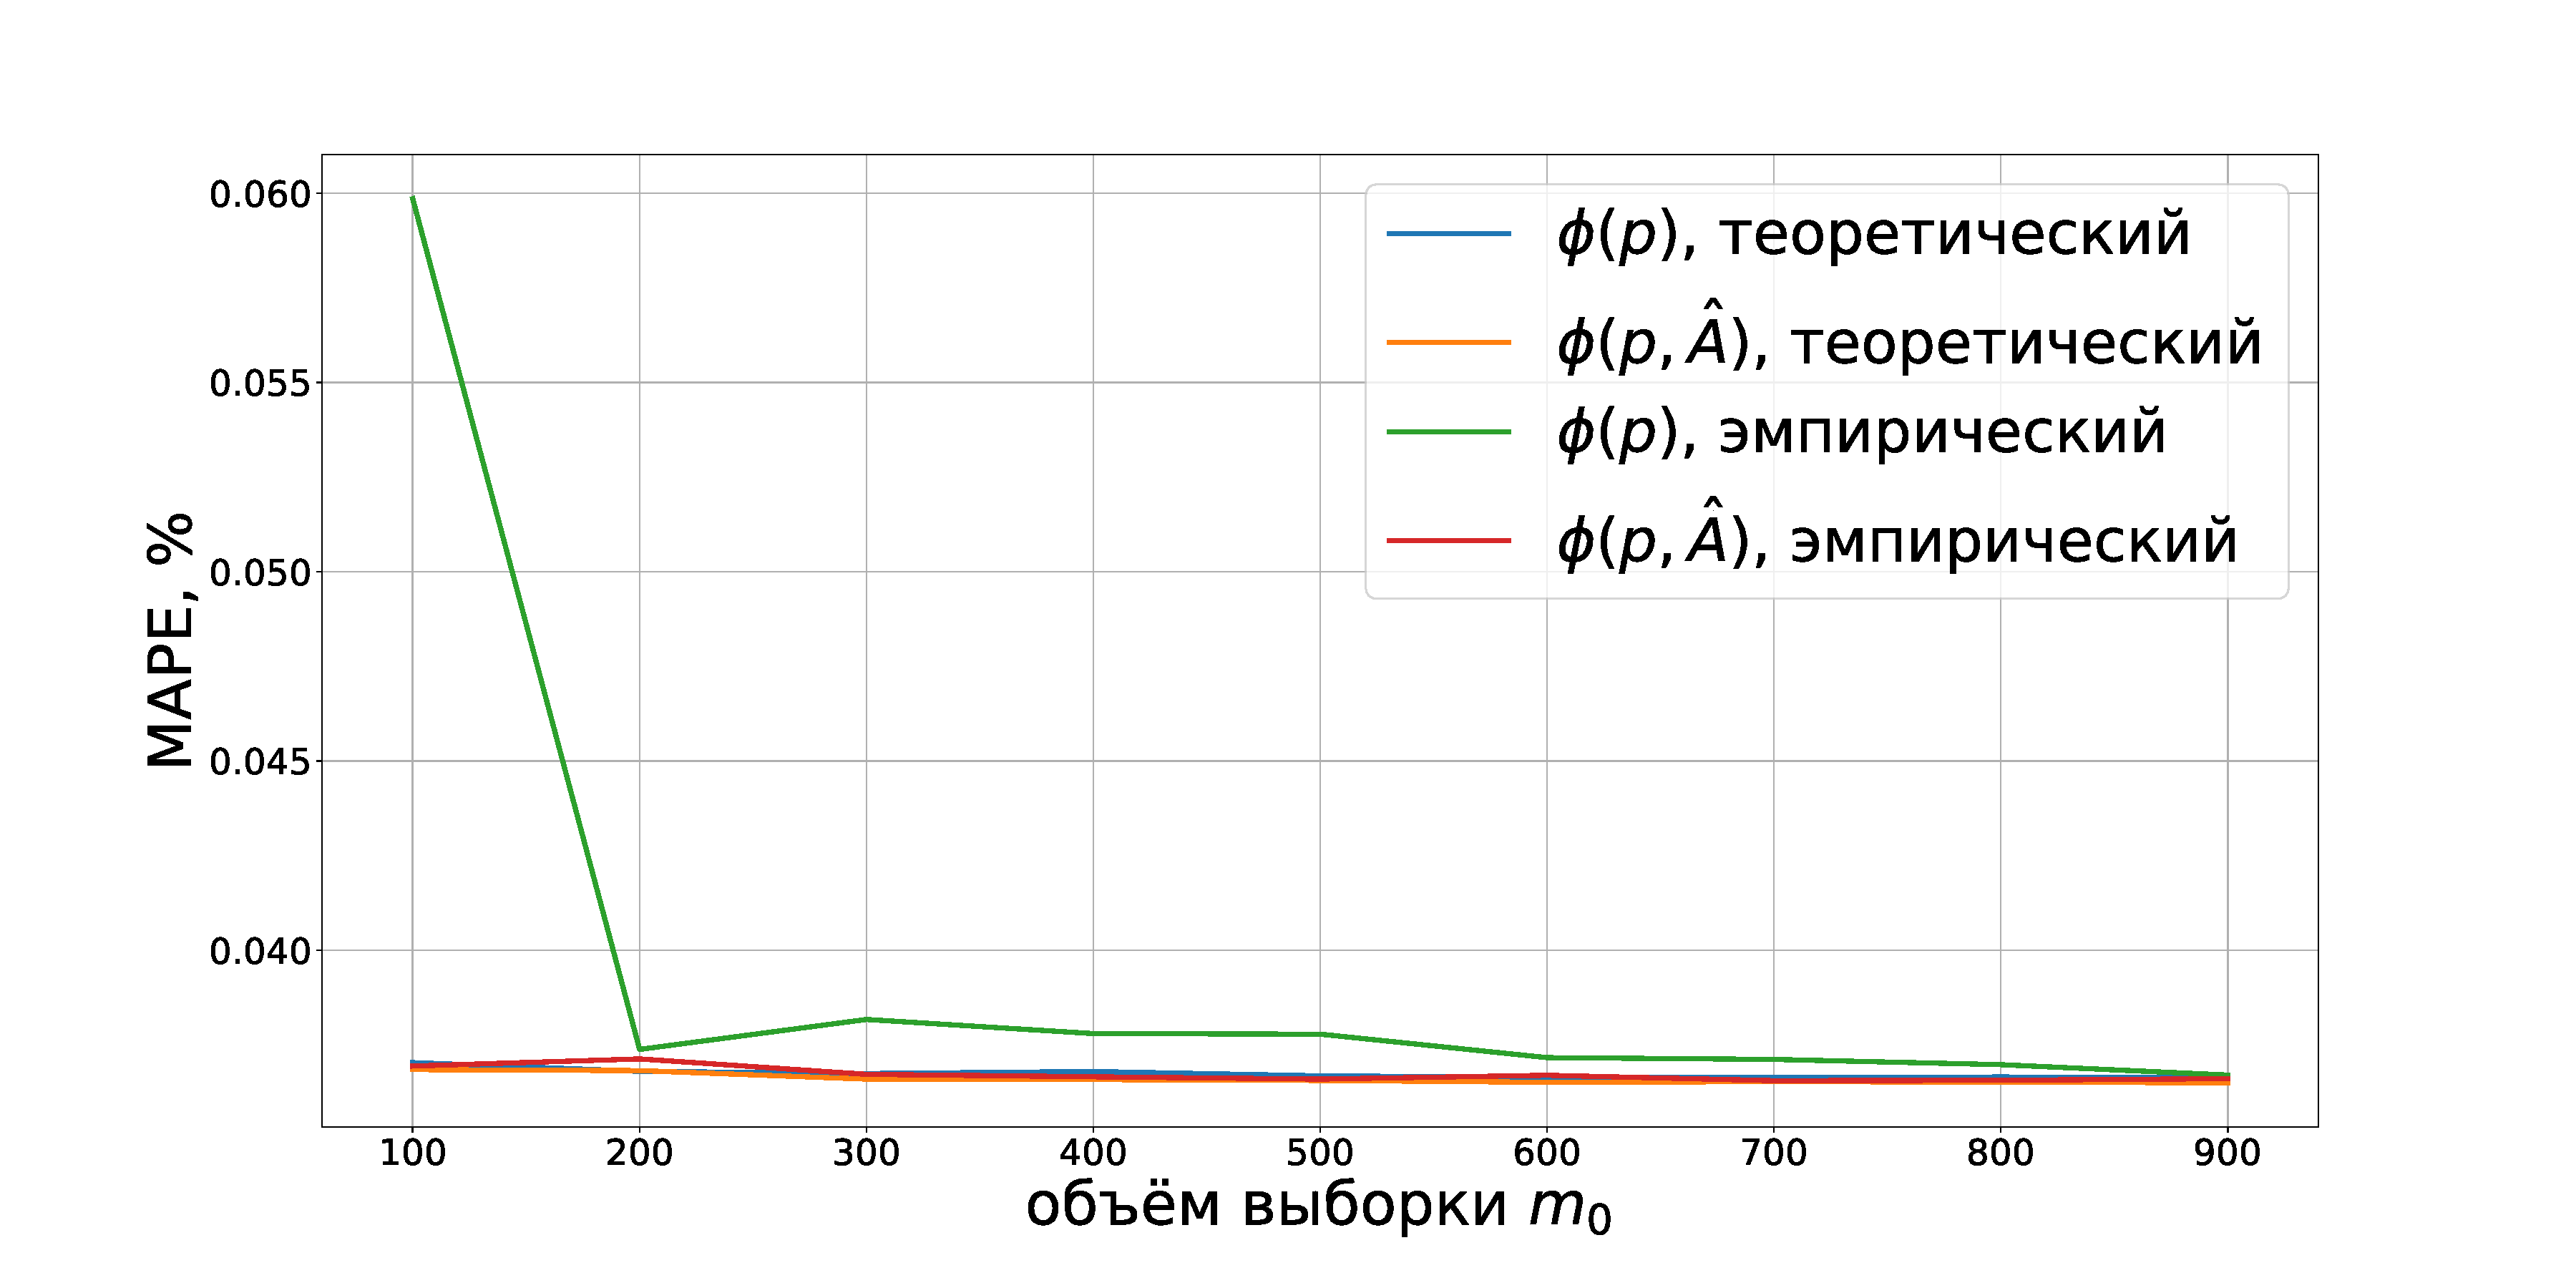
\includegraphics[width=0.5\textwidth]{../data/pics/adequate_random_sample_MAPE_comparison.pdf}}&
\subfloat[Случайная выборка]{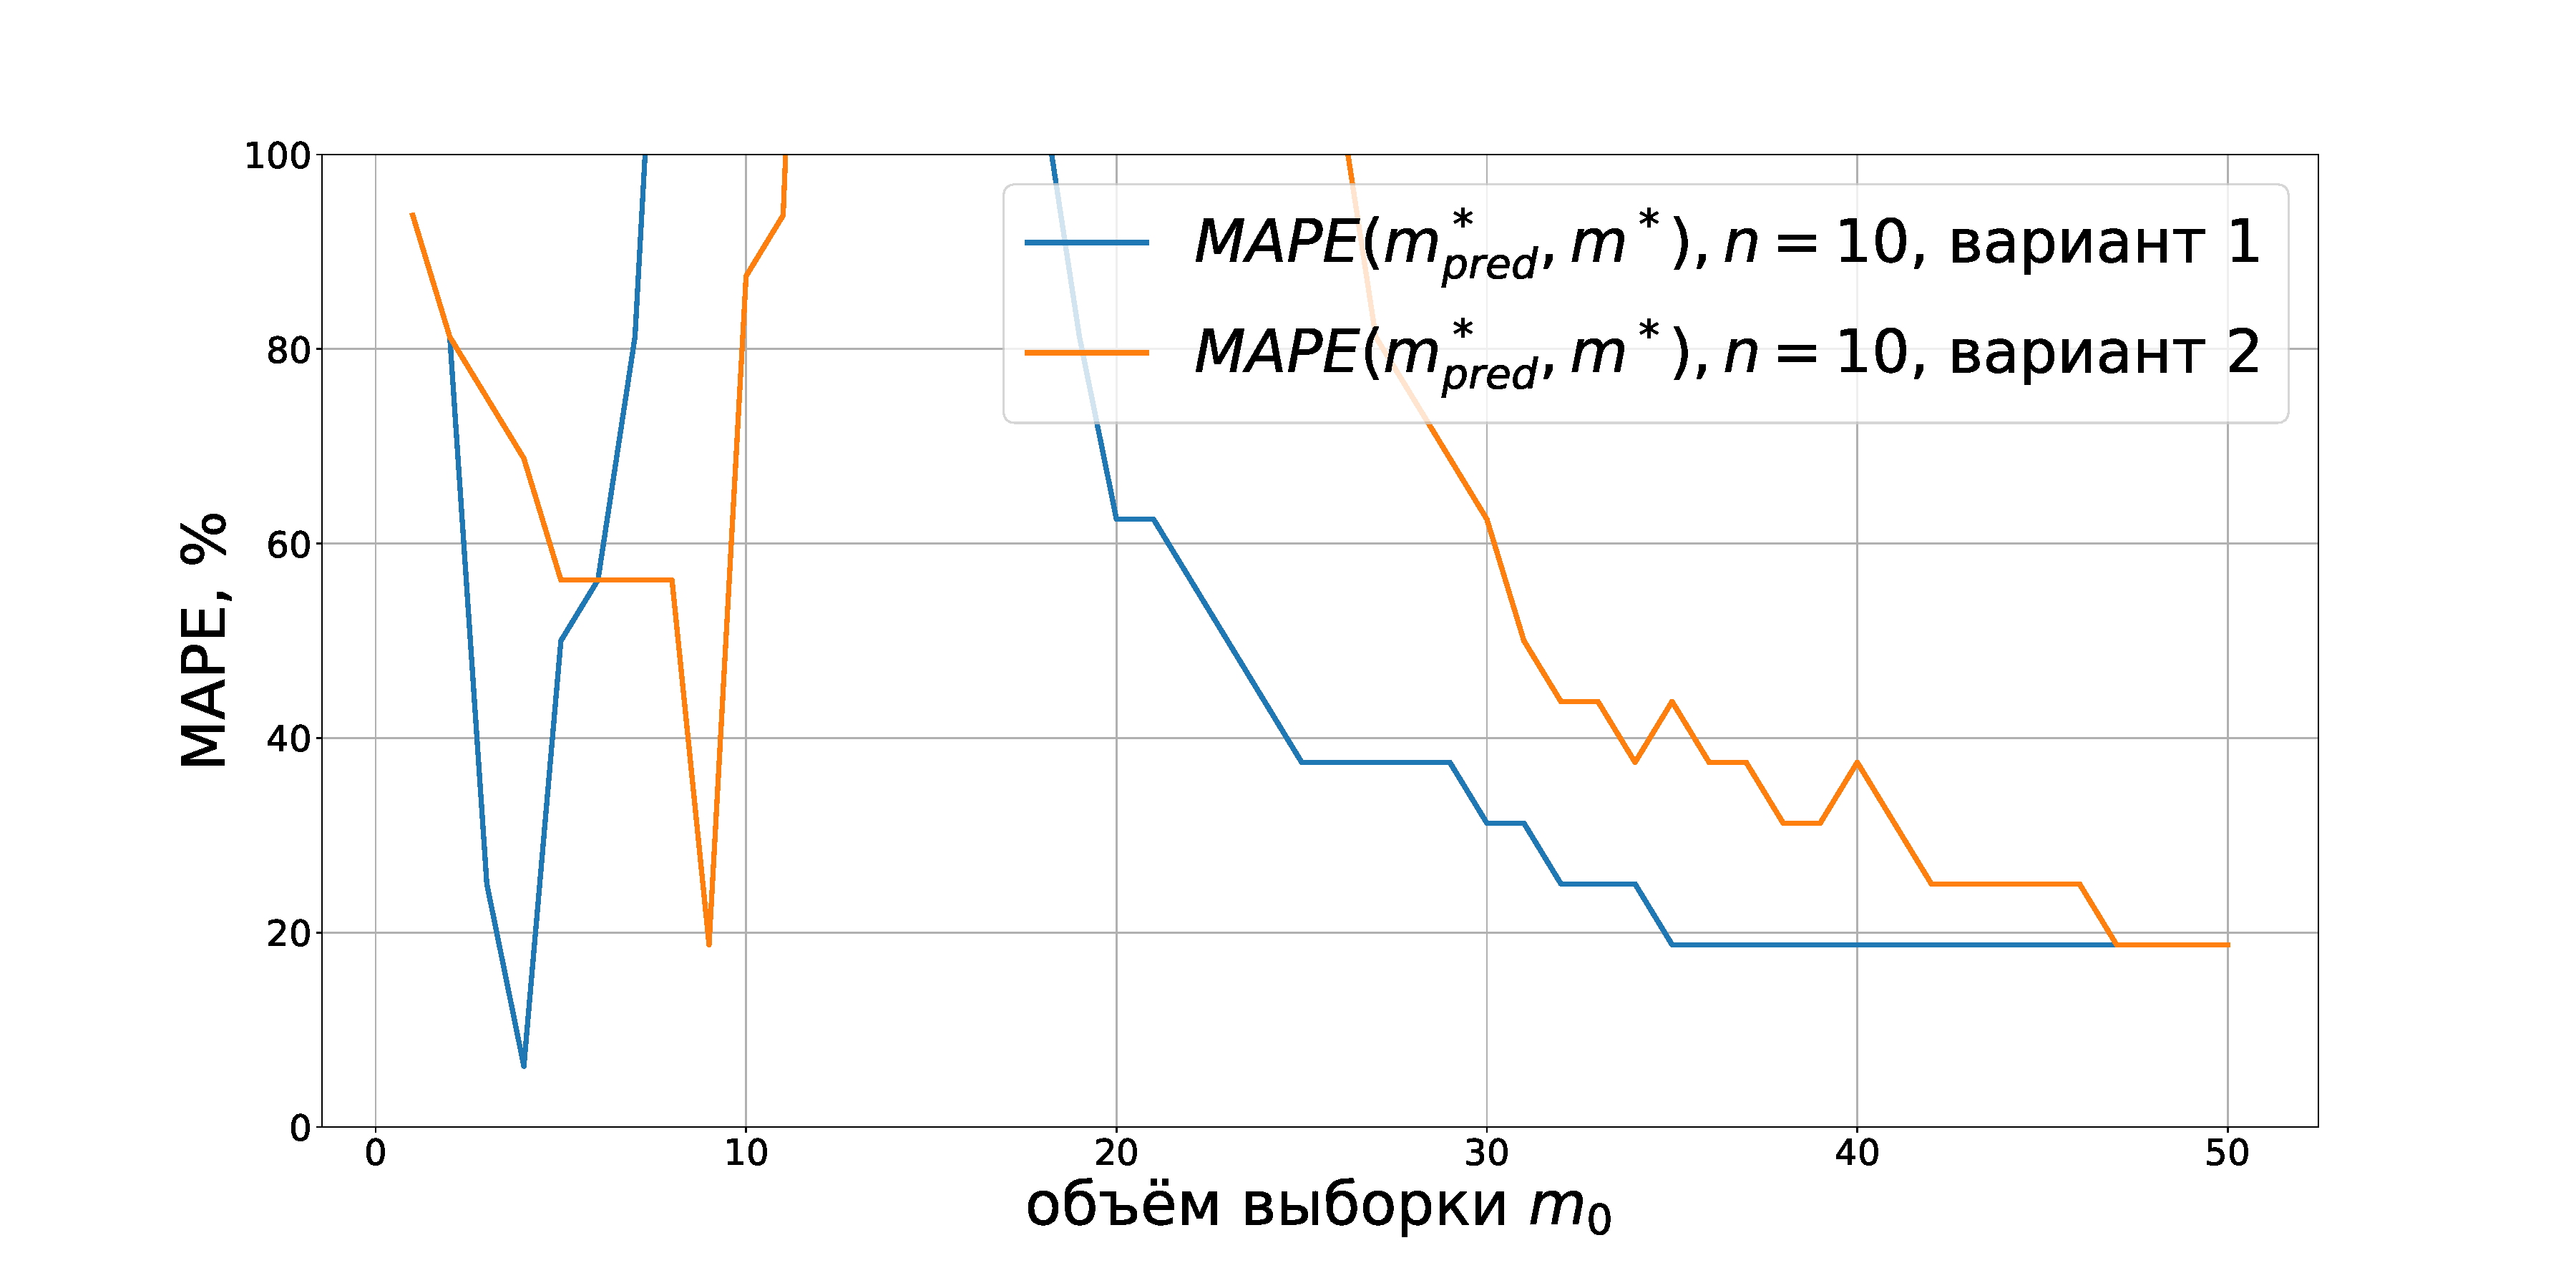
\includegraphics[width=0.5\textwidth]{../data/pics/adequate_random_sample_MAPE_m_comparison_n10.pdf}}\\
\subfloat[Скоррелированная выборка]{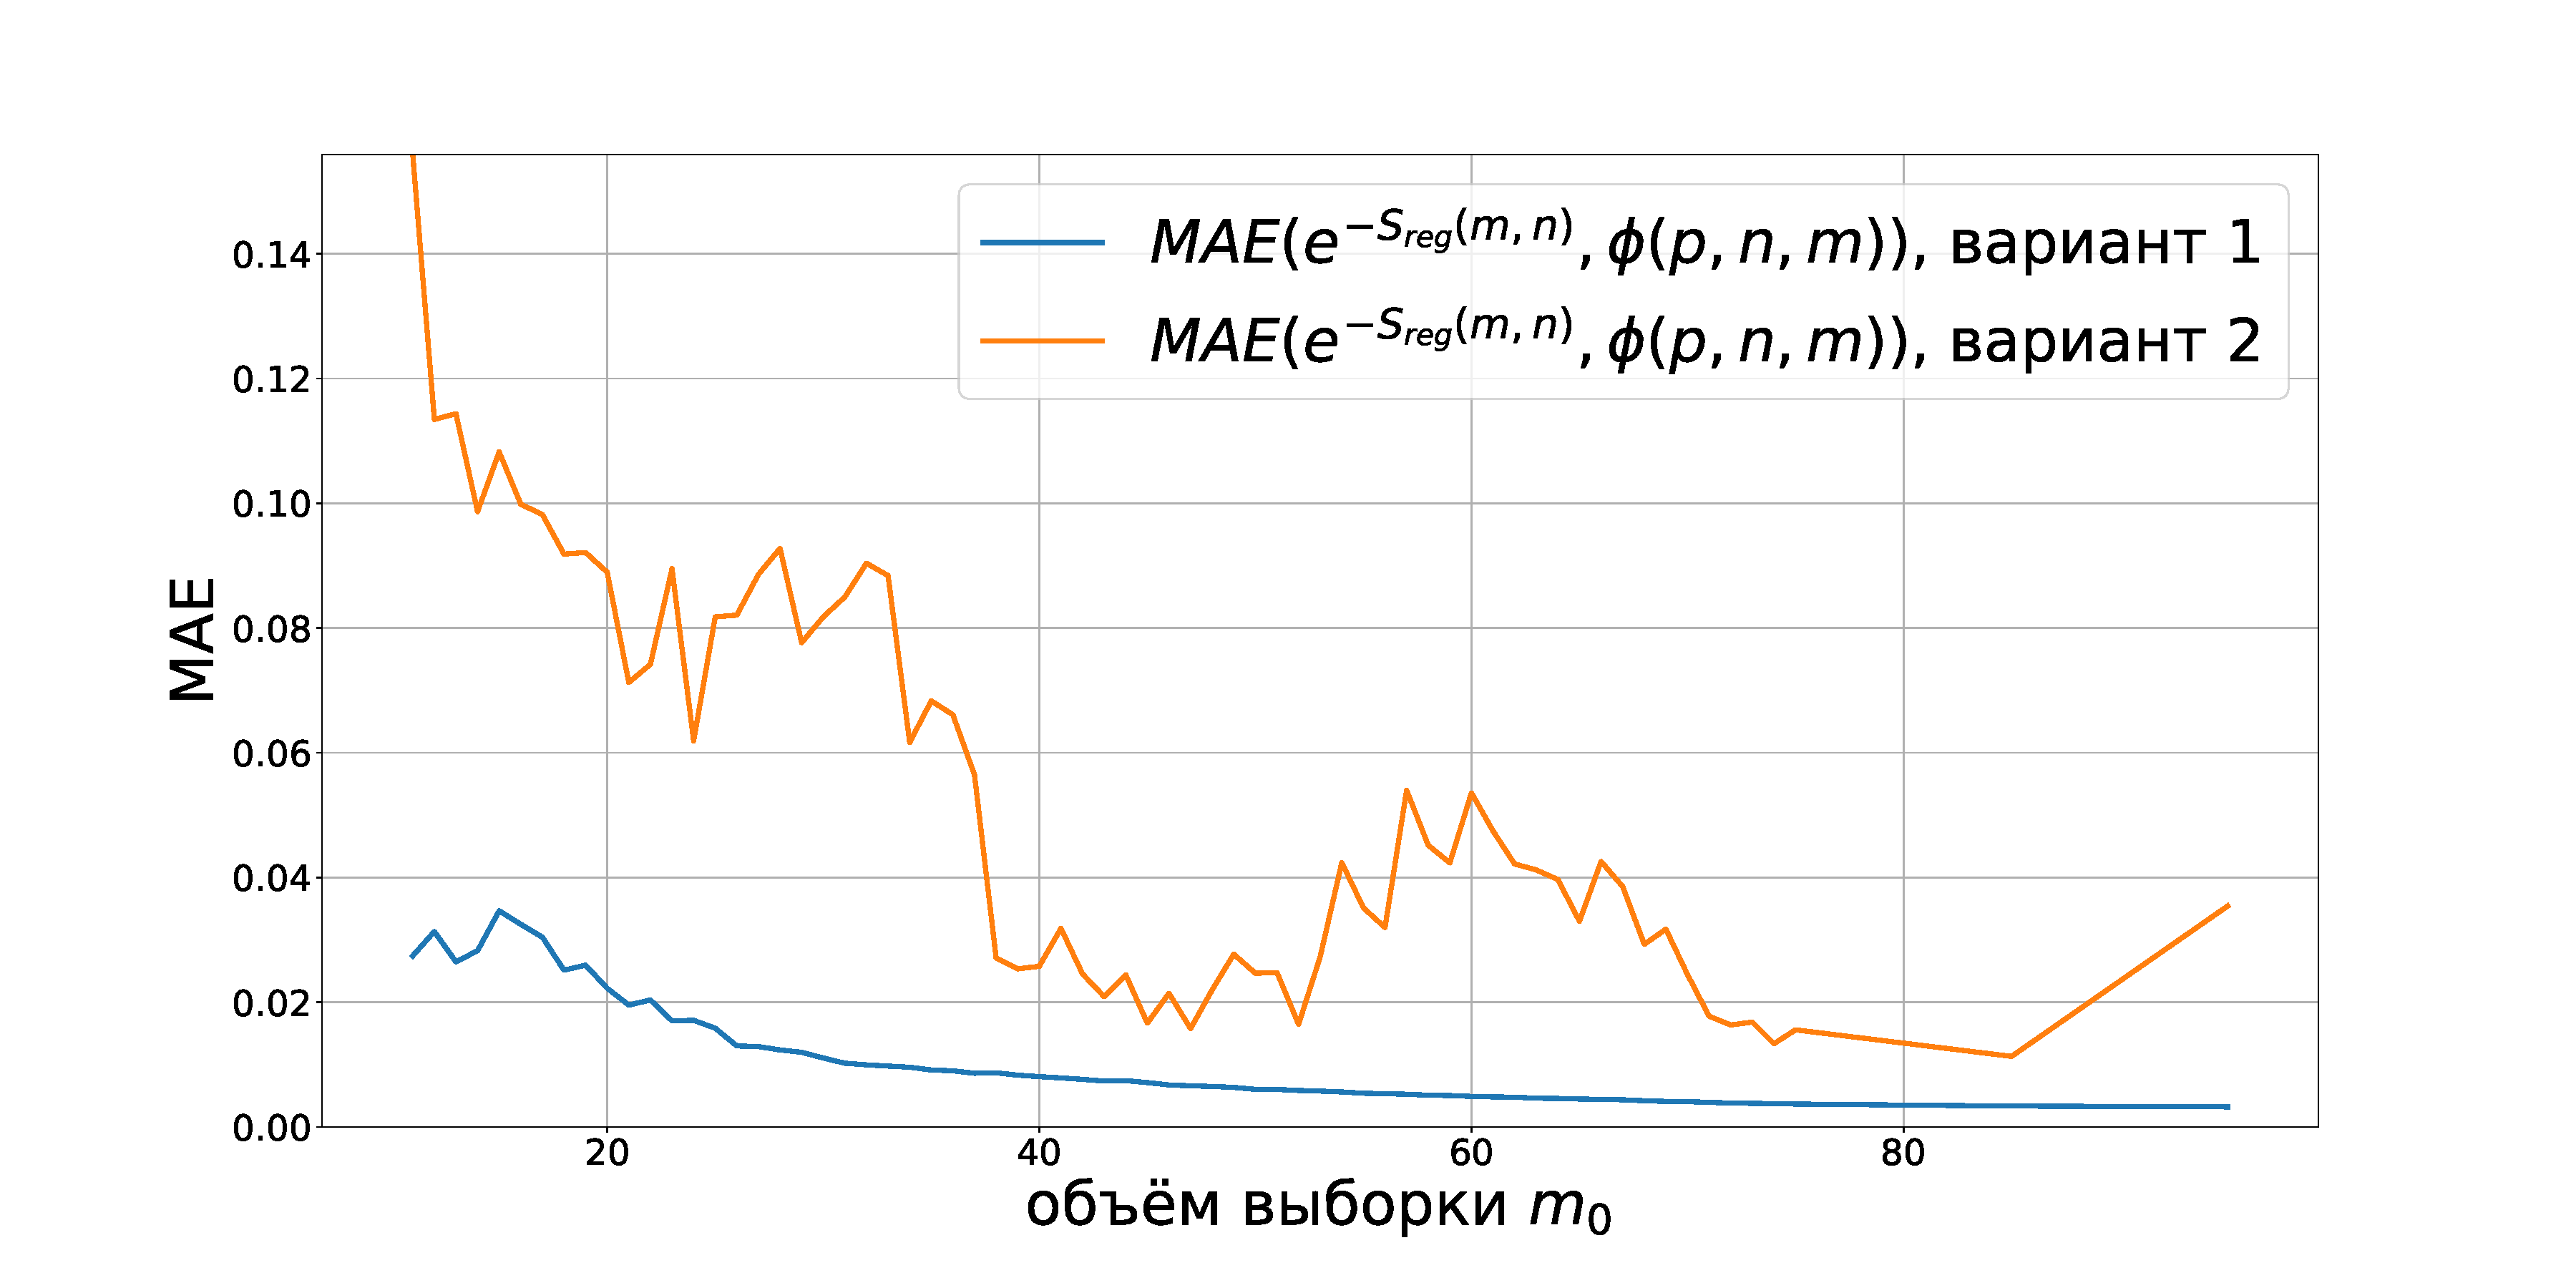
\includegraphics[width=0.5\textwidth]{../data/pics/adequate_correlated_sample_MAPE_comparison.pdf}}&
\subfloat[Скоррелированная выборка]{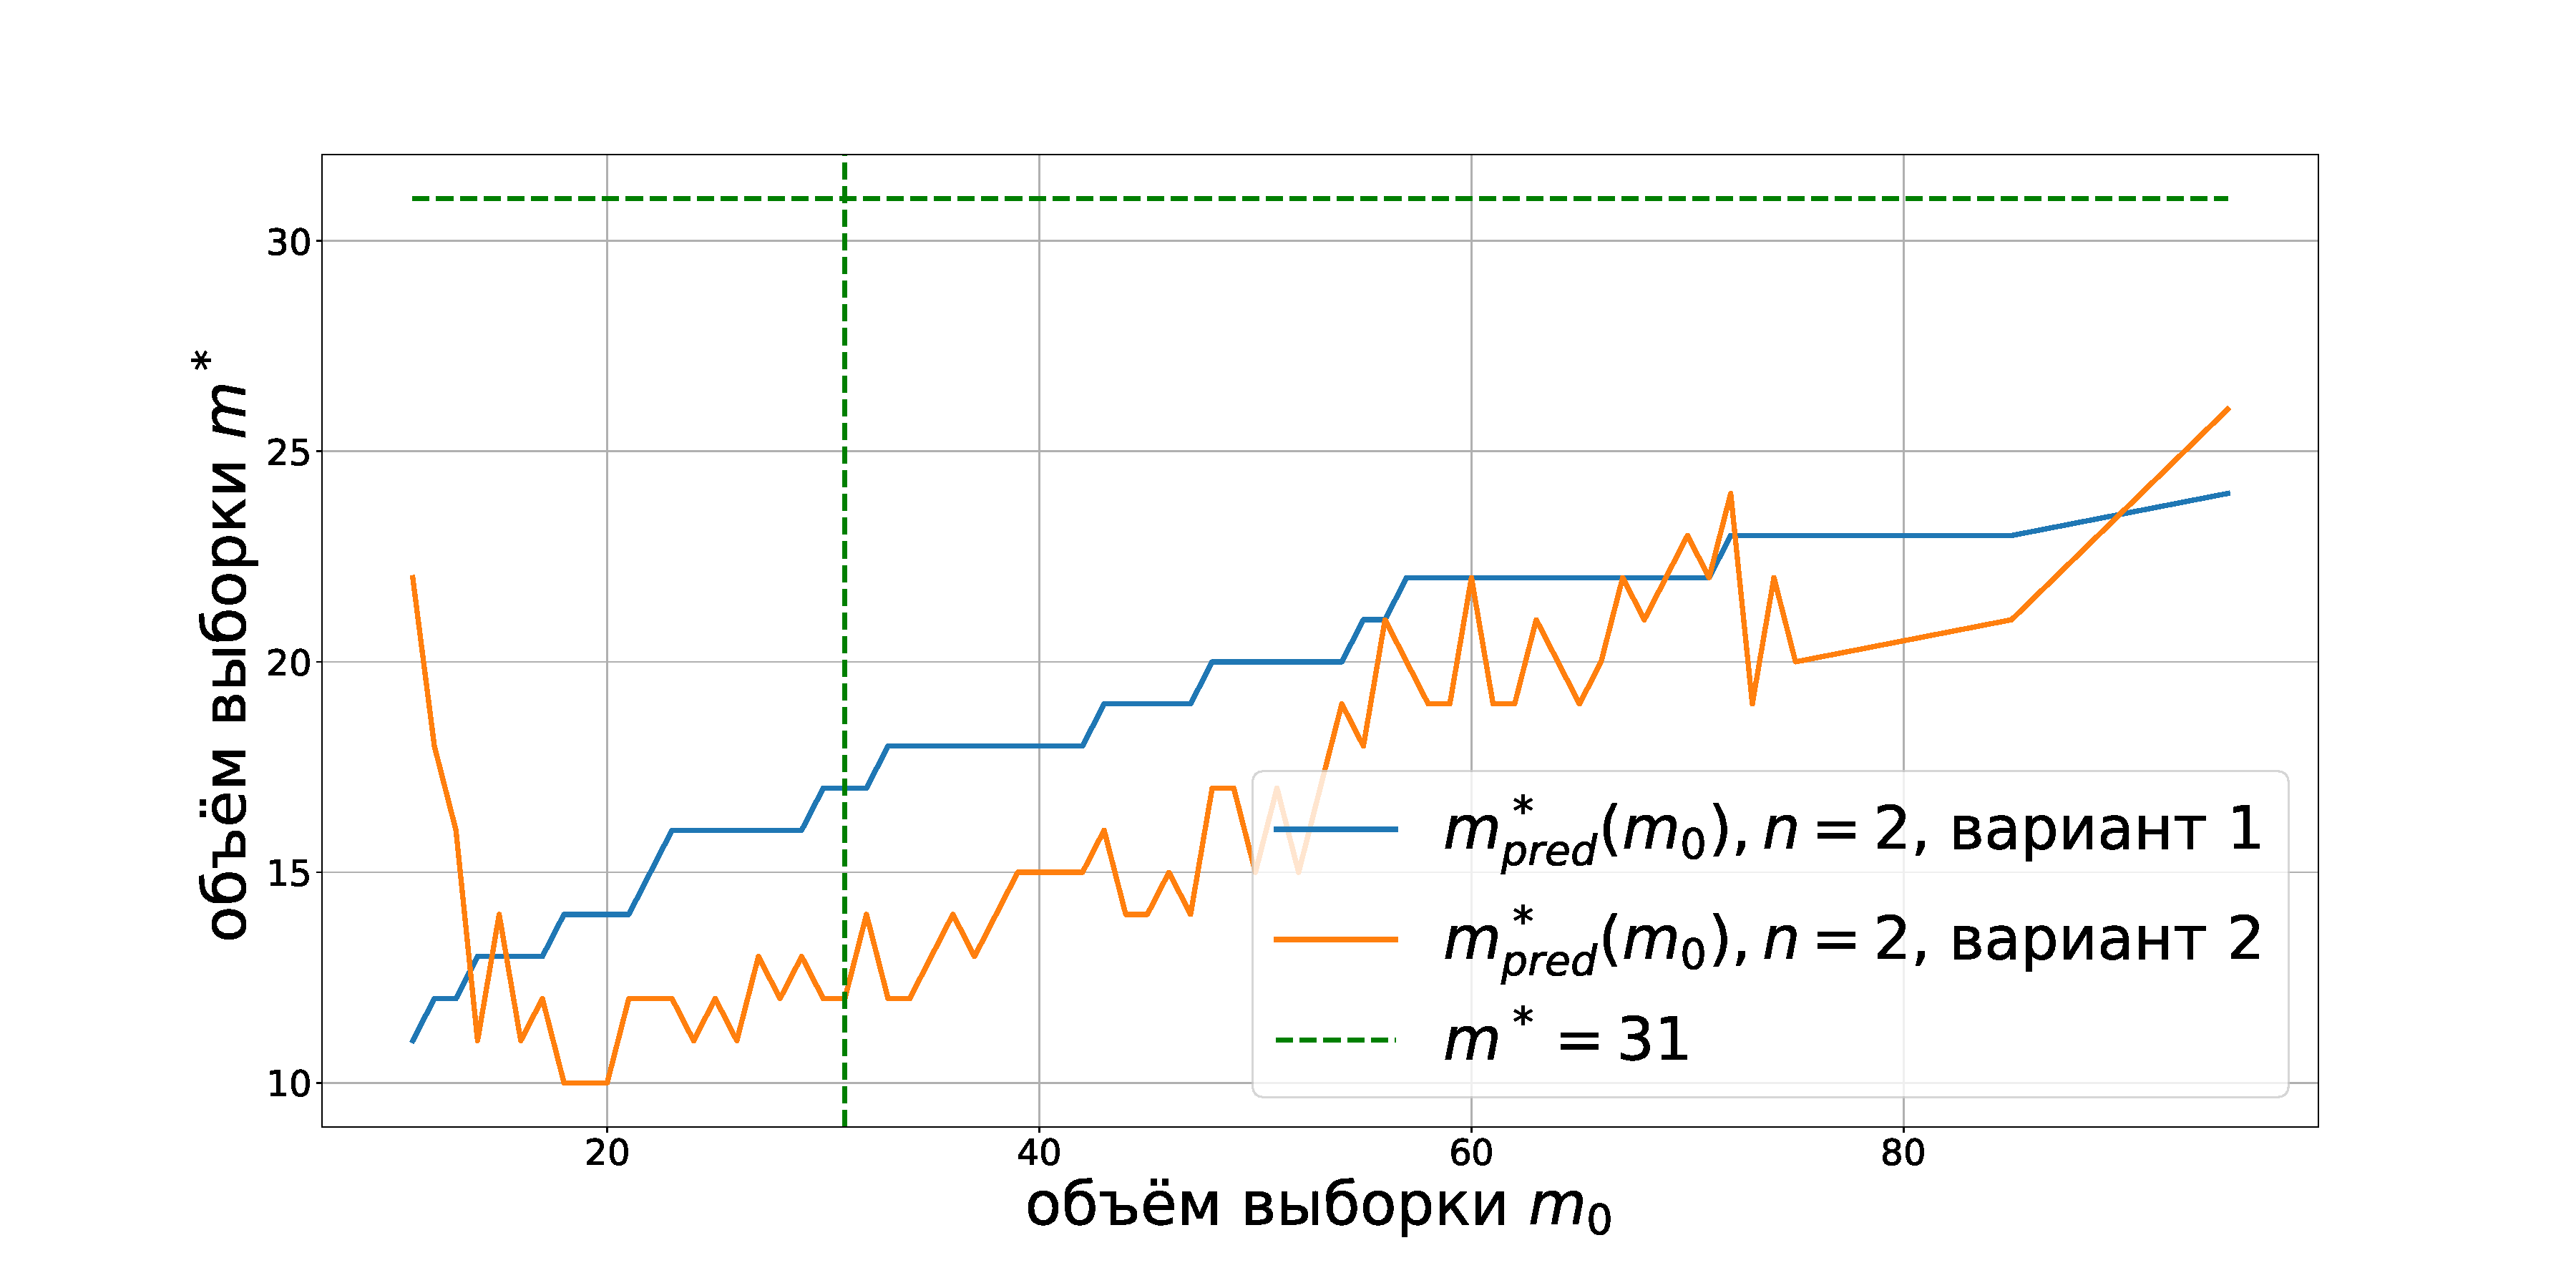
\includegraphics[width=0.5\textwidth]{../data/pics/adequate_correlated_sample_MAPE_m_comparison_n2.pdf}}\\
\subfloat[Ортогональная выборка]{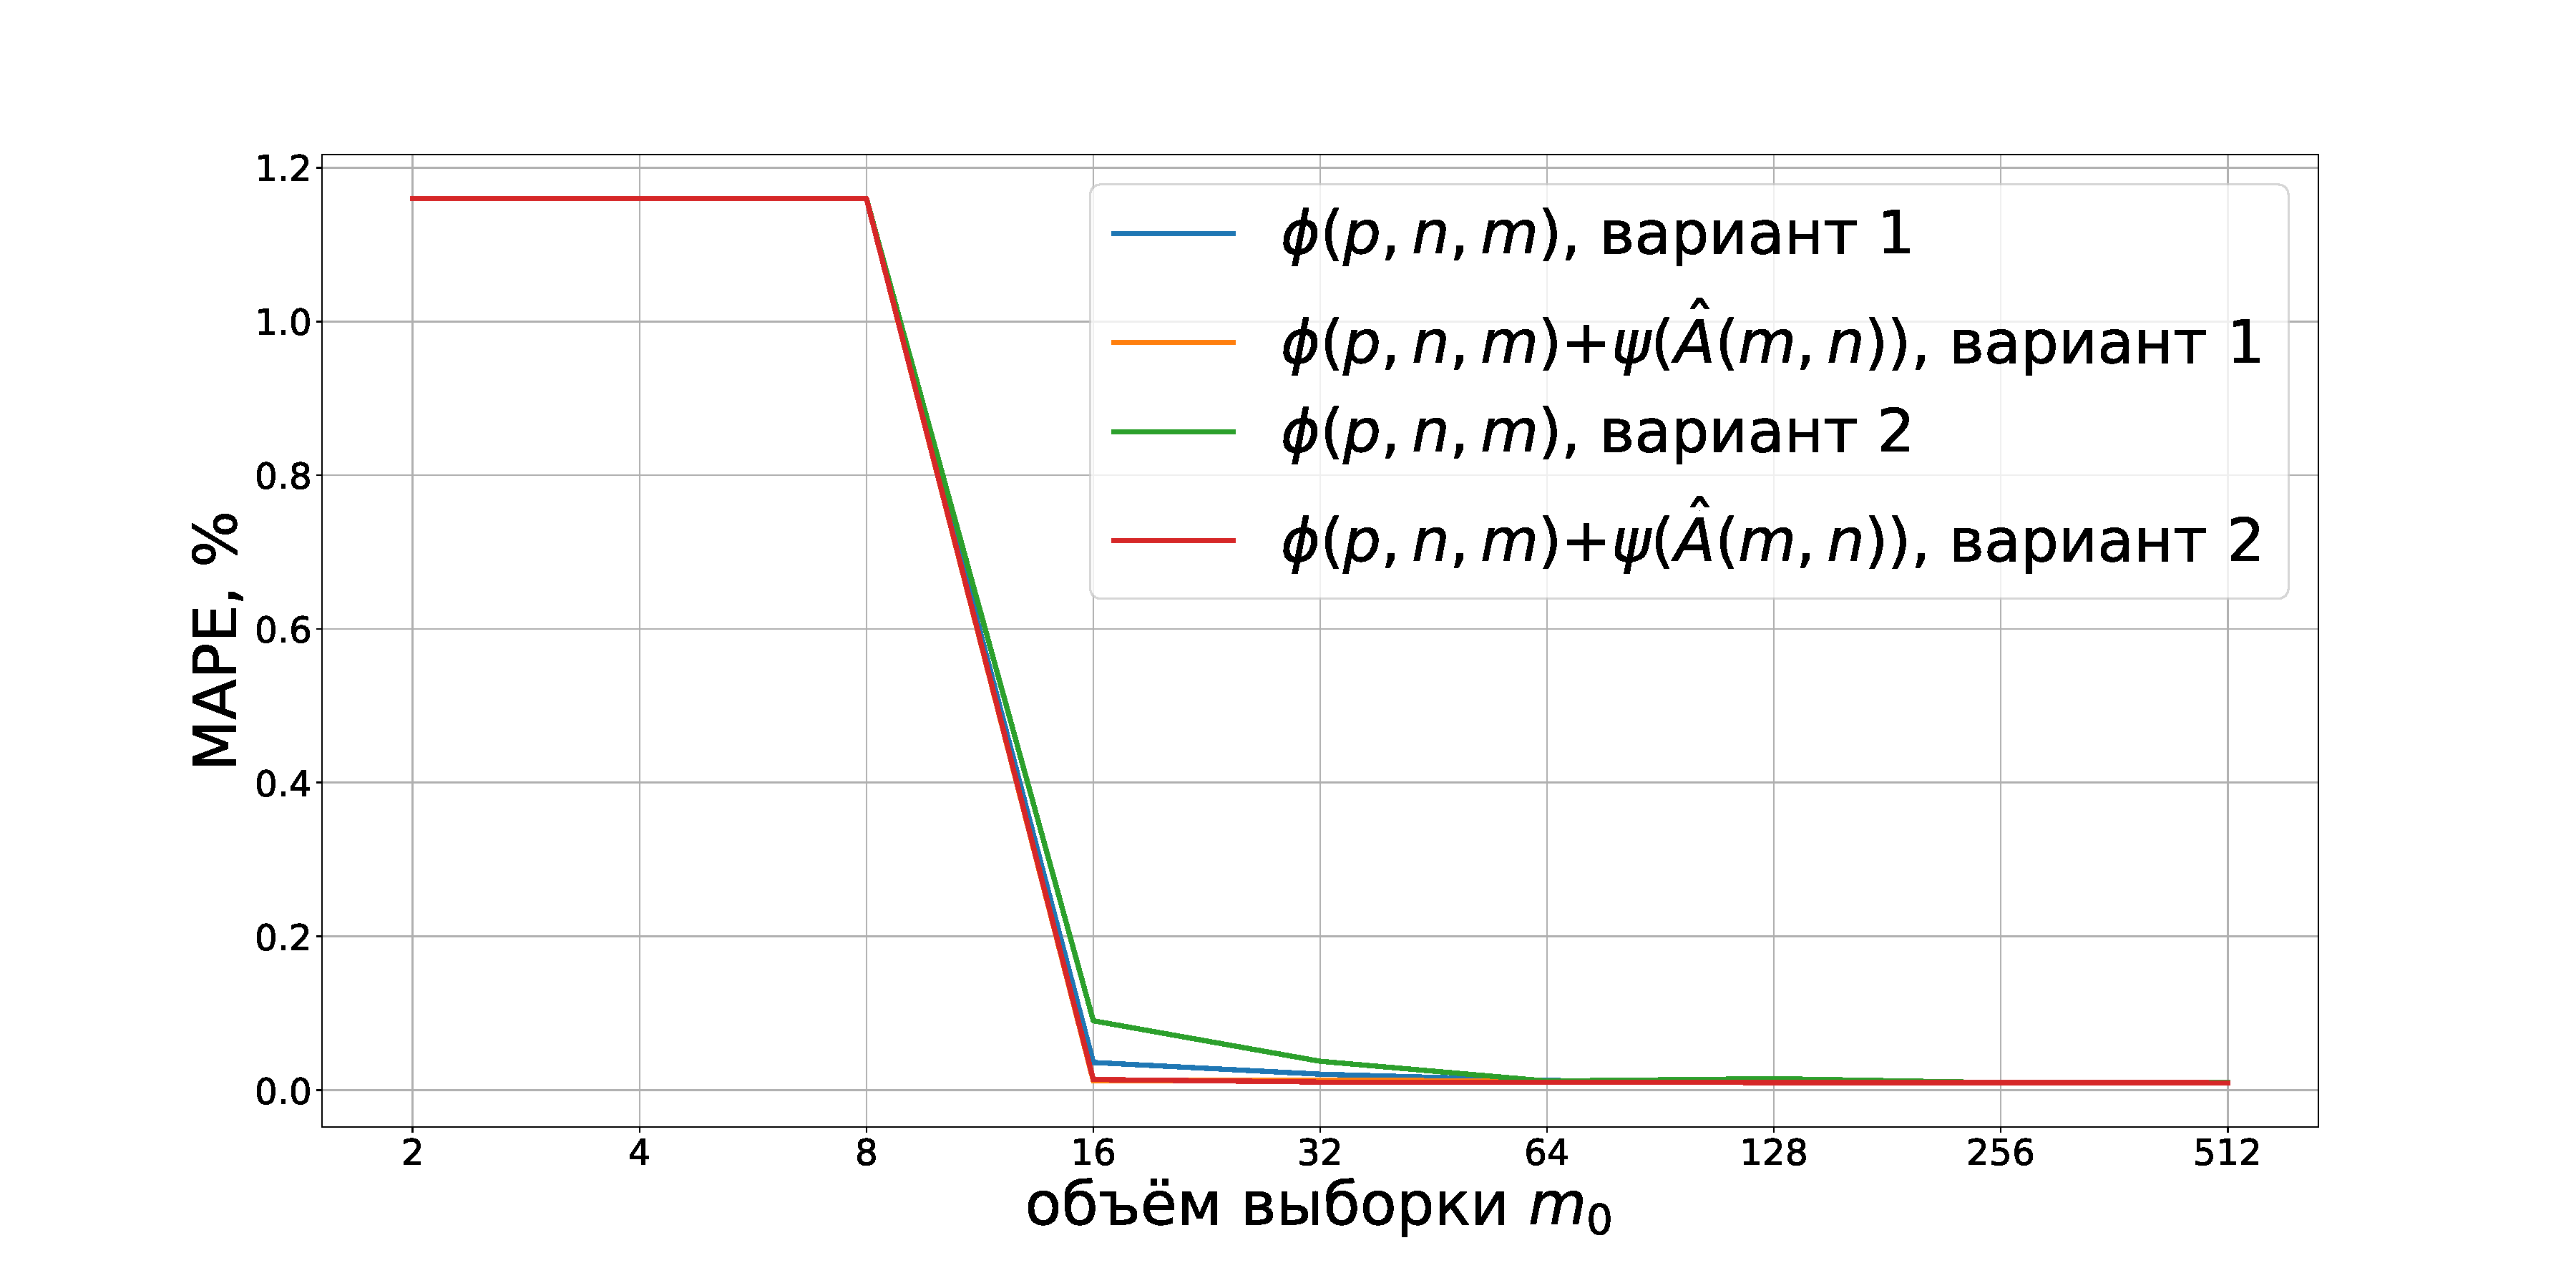
\includegraphics[width=0.5\textwidth]{../data/pics/adequate_orthogonal_sample_MAPE_comparison.pdf}}&
\subfloat[Ортогональная выборка]{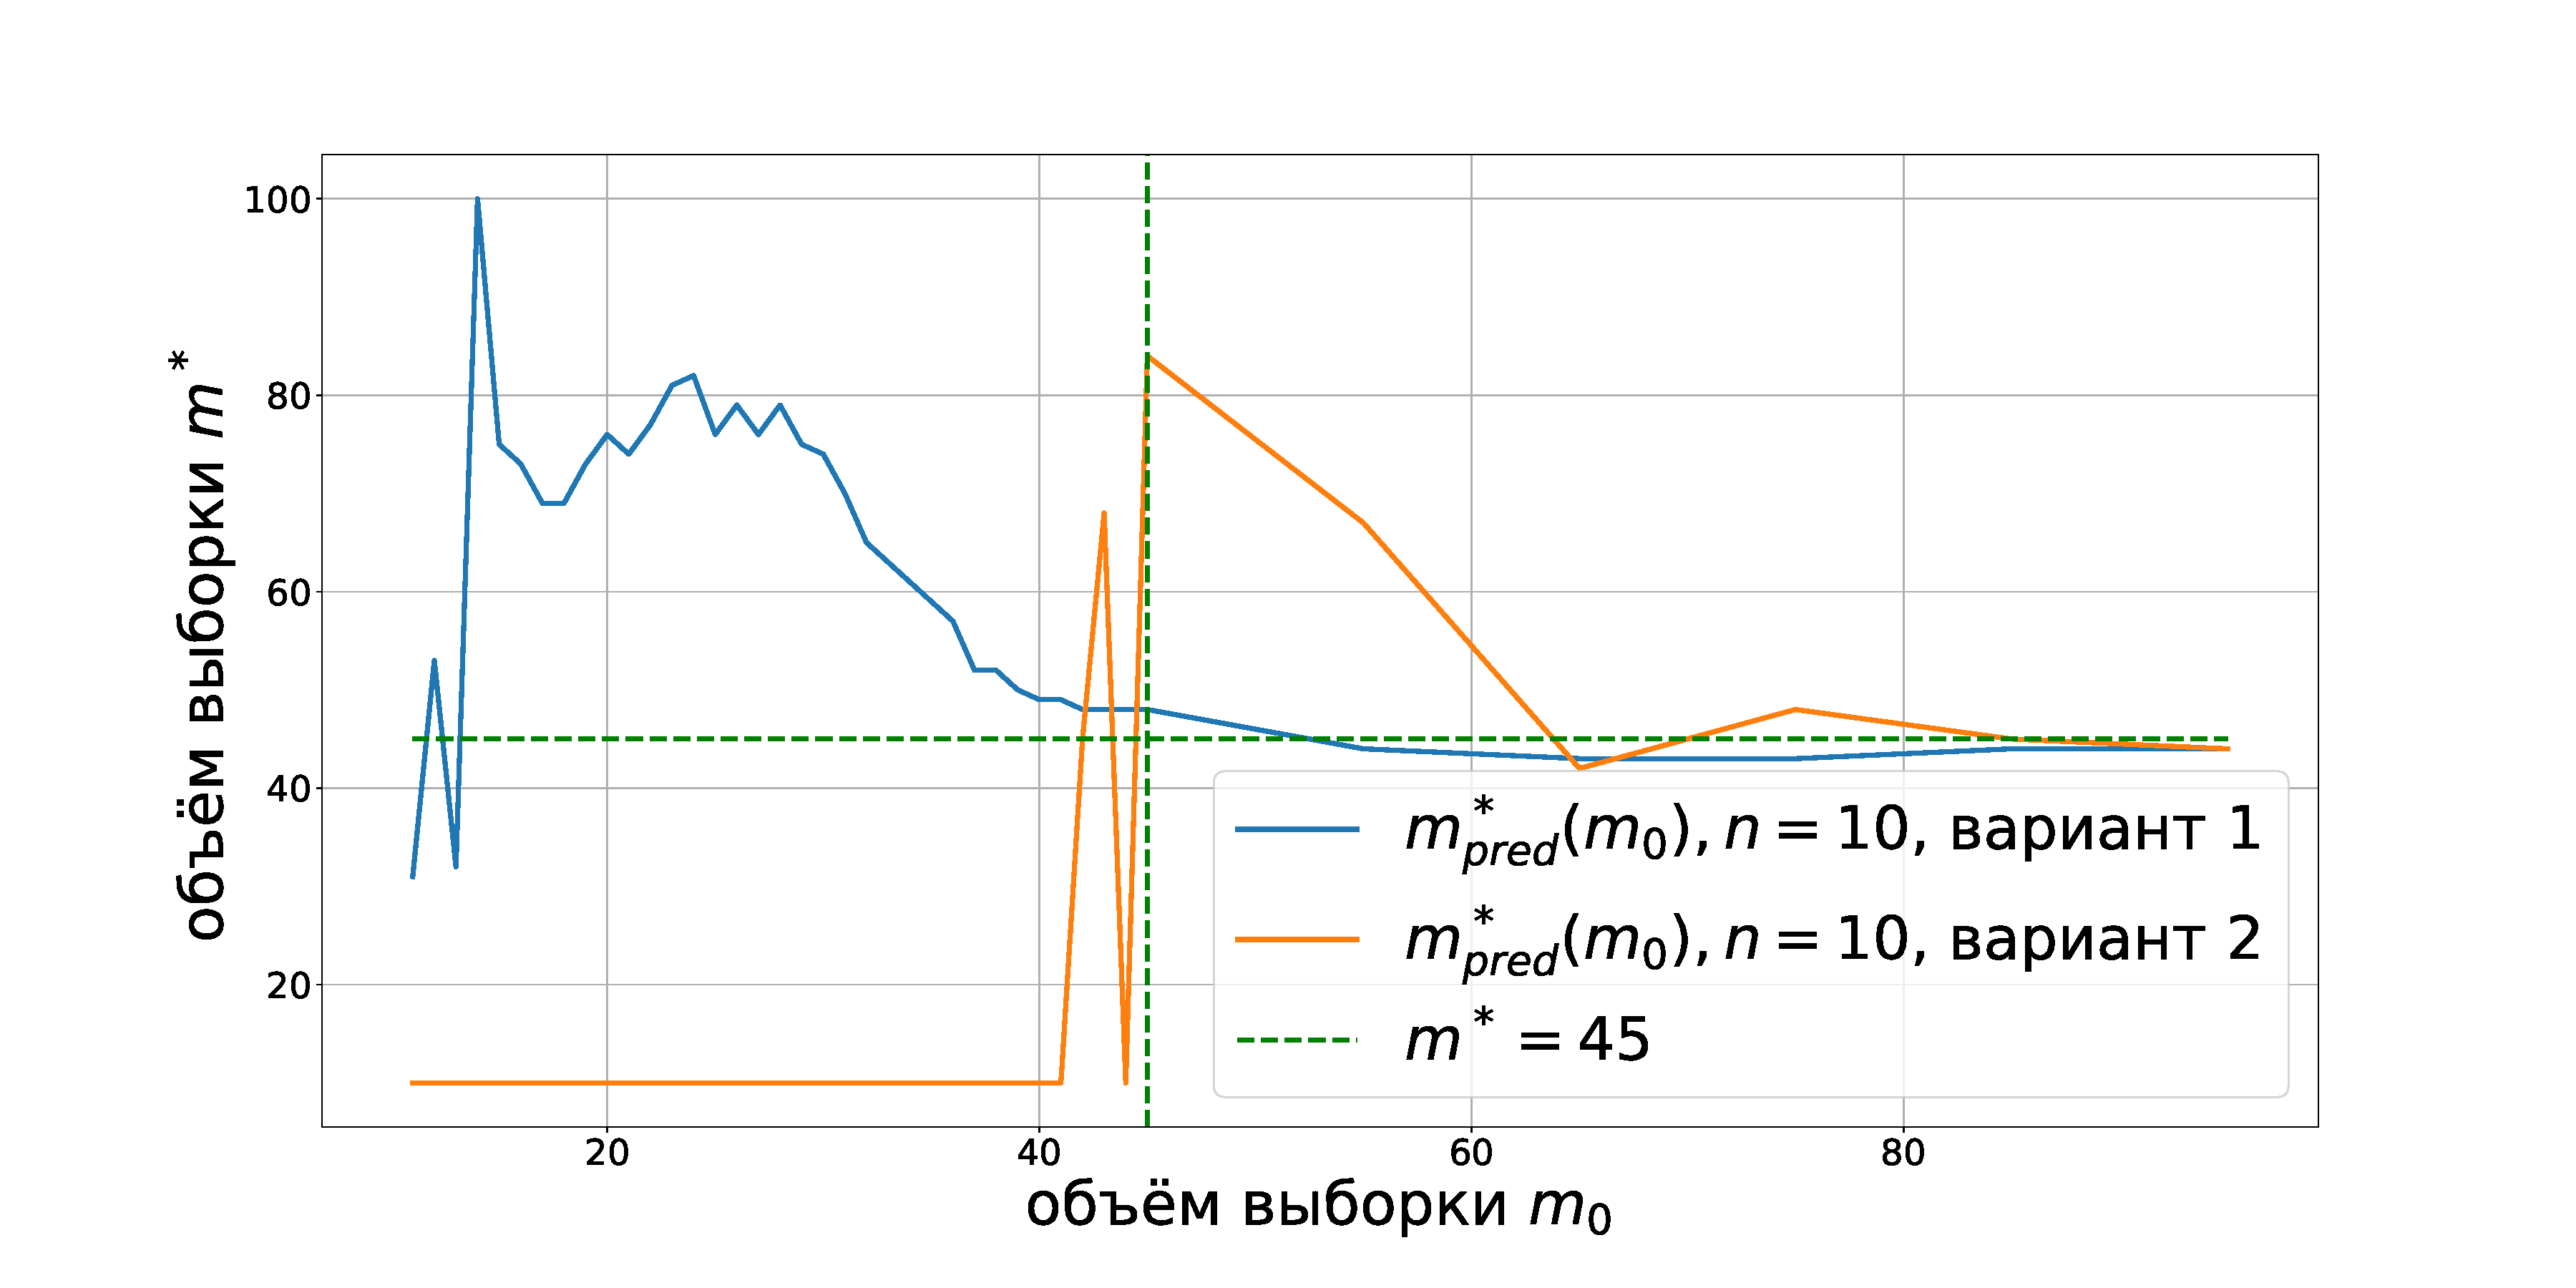
\includegraphics[width=0.5\textwidth]{../data/pics/adequate_orthogonal_sample_MAPE_m_comparison_n10.pdf}}\\
\subfloat[Избыточная выборка]{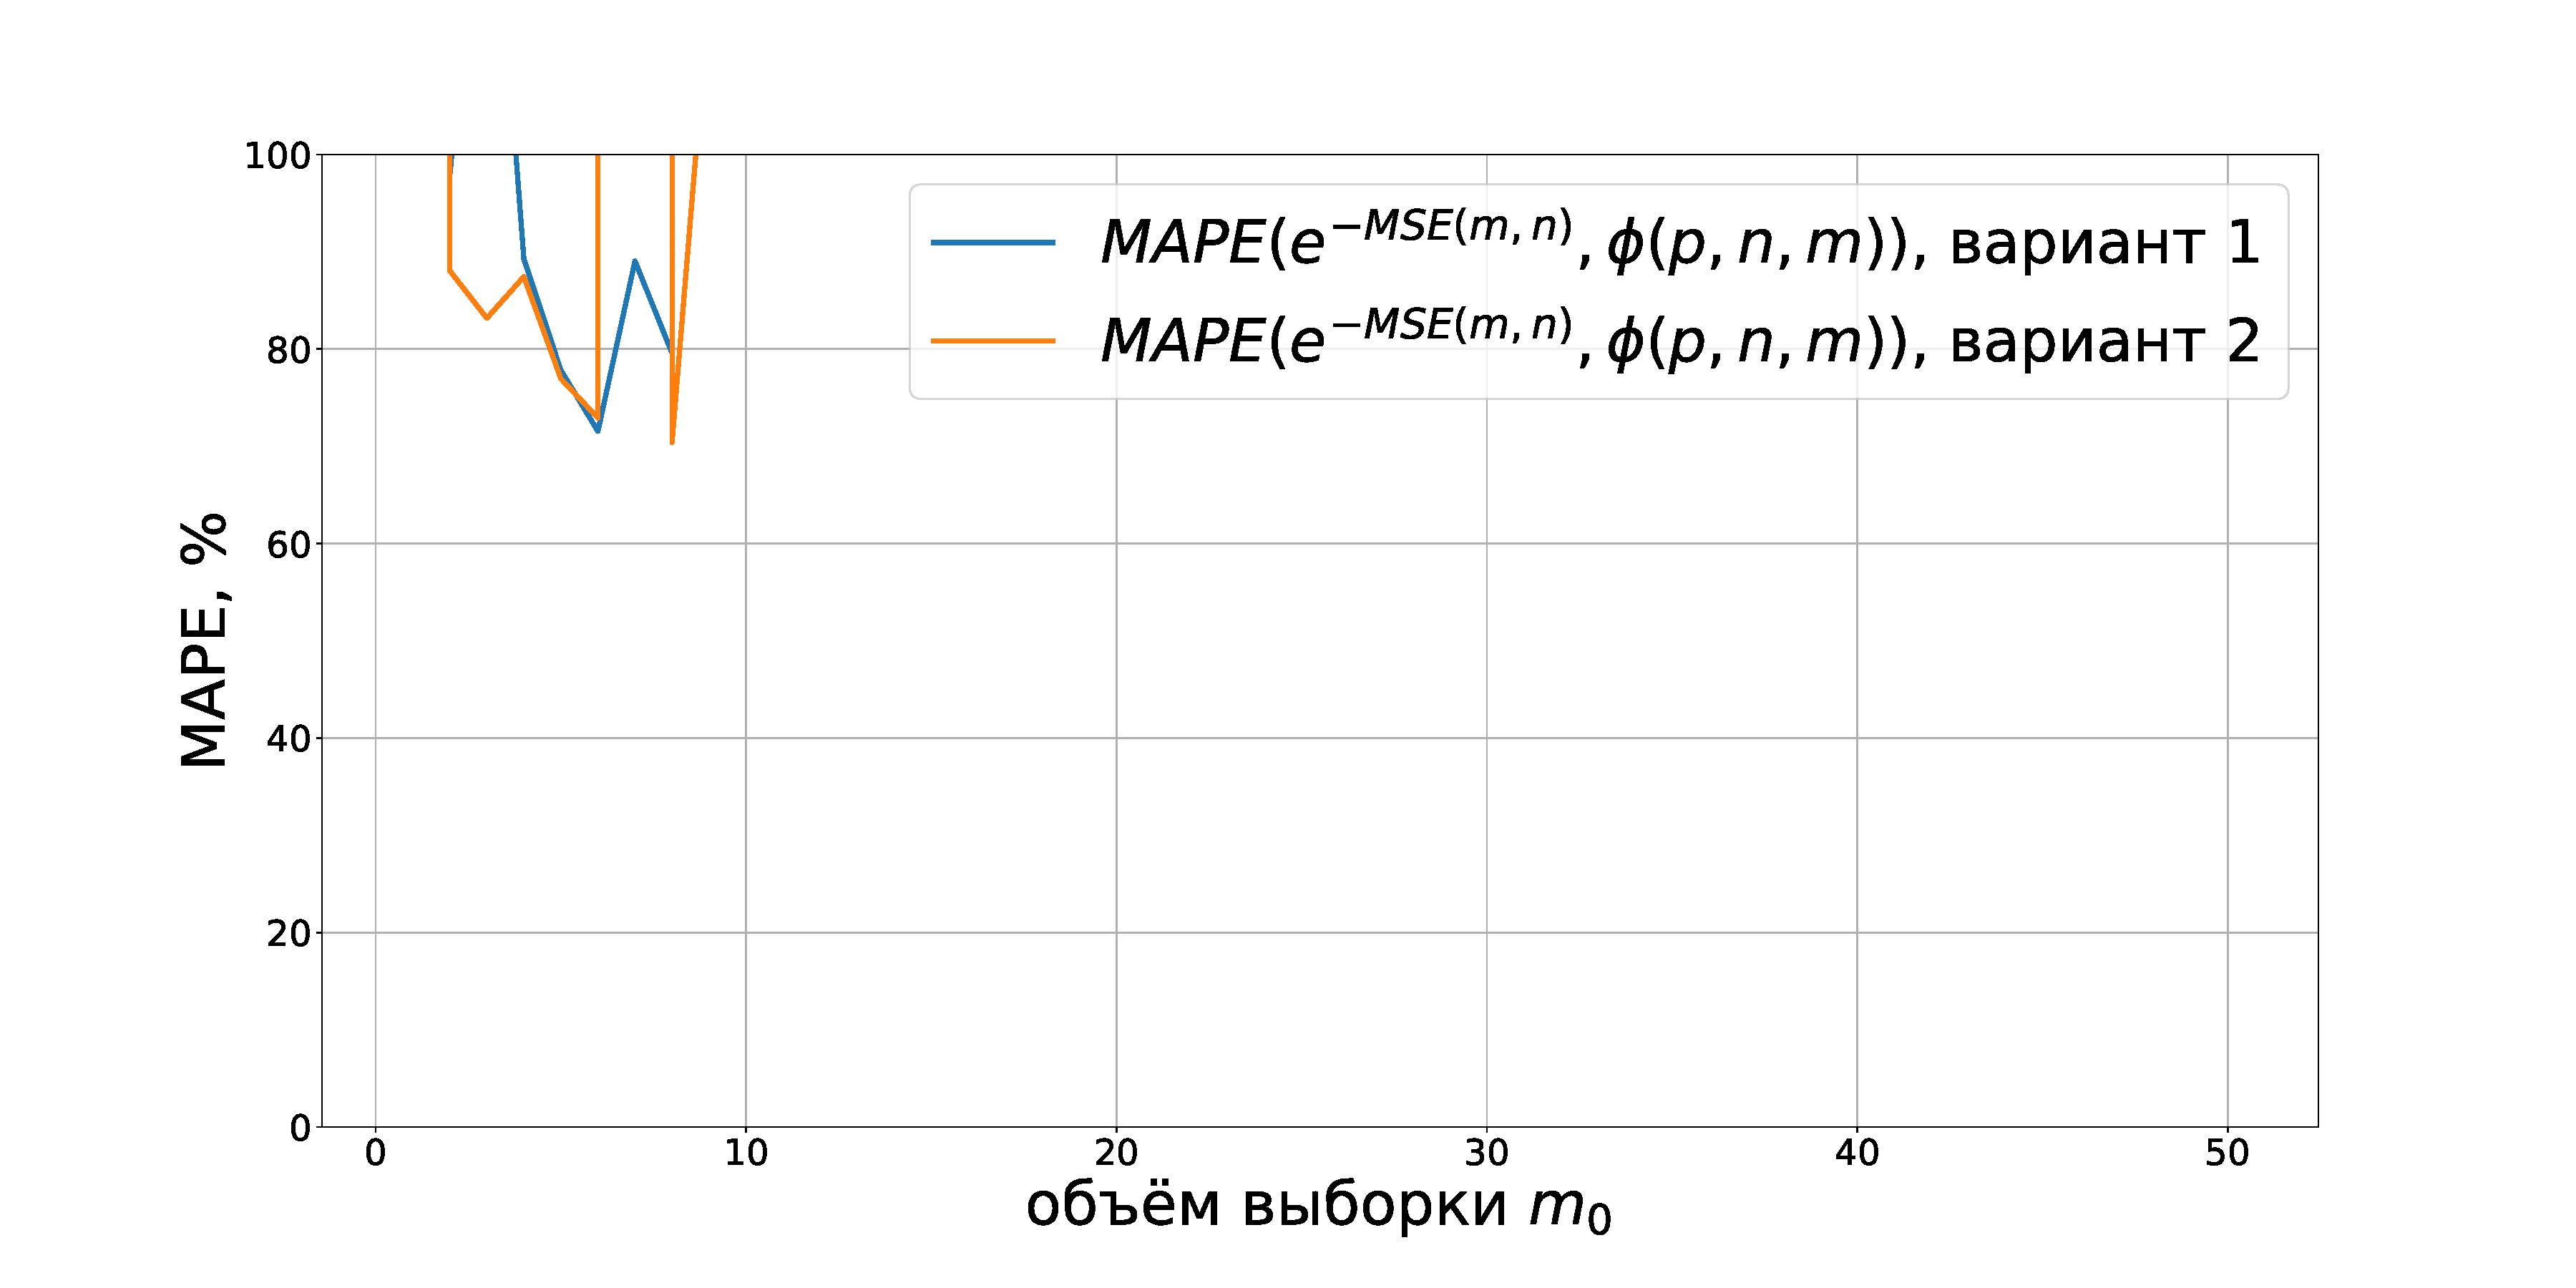
\includegraphics[width=0.5\textwidth]{../data/pics/adequate_redundant_sample_MAPE_comparison.pdf}}&
\subfloat[Избыточная выборка]{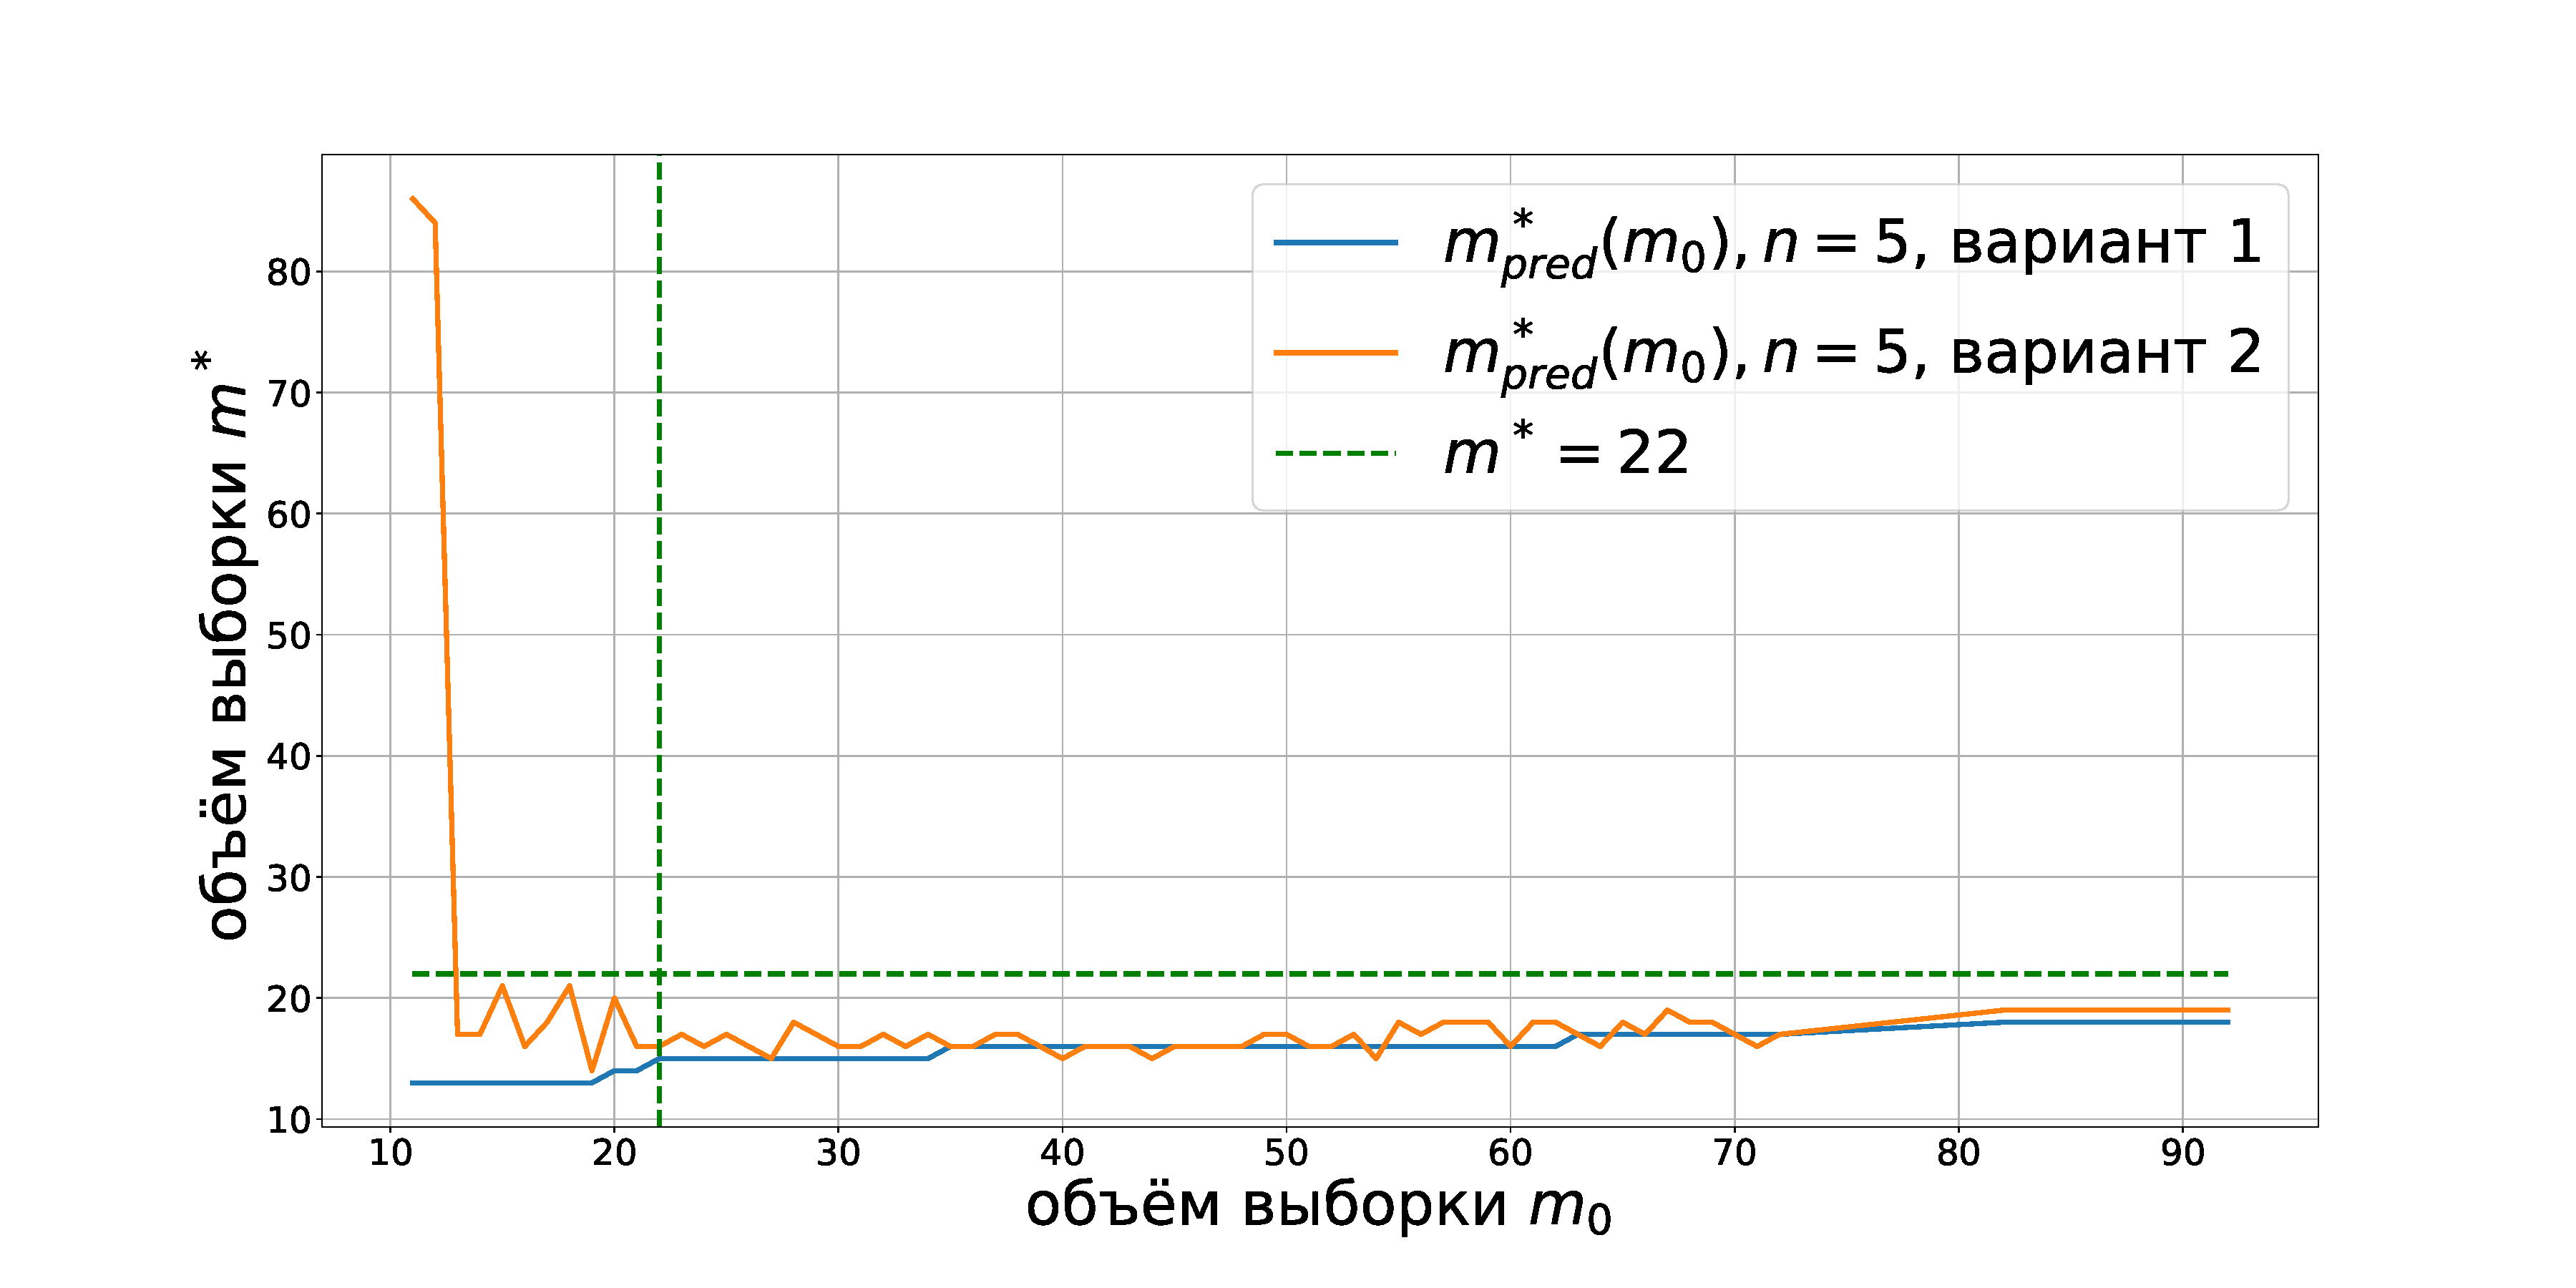
\includegraphics[width=0.5\textwidth]{../data/pics/adequate_redundant_sample_MAPE_m_comparison_n5.pdf}}\\
\end{tabular}

\caption{Качество предсказания $e^{-S(m, n)}$ и $m^*$ в зависимости от объема обучающей выборки $m_0$ для синтетических выборок}
\label{fig2}
\end{figure}

\subsection{Эксперимент на выборках из UCI репозитория}

Для эксперимента использовались выборки из UCI репозитория, описанные в табл. 2. 

\begin{table}[h]
\begin{center}
\caption{Выборки из UCI репозитория}
\label{table2}
\begin{tabularx}{0.7\textwidth}{|c|>{\centering\arraybackslash}X|>{\centering\arraybackslash}X|>{\centering\arraybackslash}X|}
\hline
	\centering Выборка & Тип задачи & $m$ & $n$\\
	\hline
	Diabetes & регрессия & 442 & 11\\
	\hline
	Boston & регрессия & 506 & 14\\
	\hline
	Wine & классификация & 130 & 14\\
	\hline
	Nba & классификация & 400 & 20\\
\hline
\end{tabularx}
\end{center}
\end{table}

На рис. 3 представлена функция $\hat{l}(m)$, посчитанная  с помощью бутстрепа в варианте с полной информацией для различного числа признаков $n^{\prime}$. Качественное поведение функции $\hat{l}(m)$ похоже на поведение данной функции для синтетических выборок и также хорошо аппроксимируется семейством функций (\ref{Phi}).

В табл. 3 приведены оптимальные значения $m^*, n^*$ для различных выборок. Примечательно, что для задачи классификации достаточный объём выборки меньше, чем для задачи регрессии.

\begin{table}[h]
\begin{center}
\caption{Оптимальные значения $m^*, n^*$ для различных синтетических выборок}
\label{table3}
\begin{tabularx}{0.7\textwidth}{|c|>{\centering\arraybackslash}X|>{\centering\arraybackslash}X|}
\hline
	\centering Выборка & $m^*$ & $n^*$\\
	\hline
	Diabetes & 96 & 11\\
	\hline
	Boston & 102 & 14\\
	\hline
	Wine & 27 & 14\\
	\hline
	Nba & 38 & 2\\
\hline
\end{tabularx}
\end{center}
\end{table}

\newpage

\begin{figure}[h!t]\center
\centering\begin{tabular}{@{}c@{ }c@{ }c@{}}
\textbf{Матожидание} & \textbf{Дисперсия}\\
\subfloat[Diabetes]{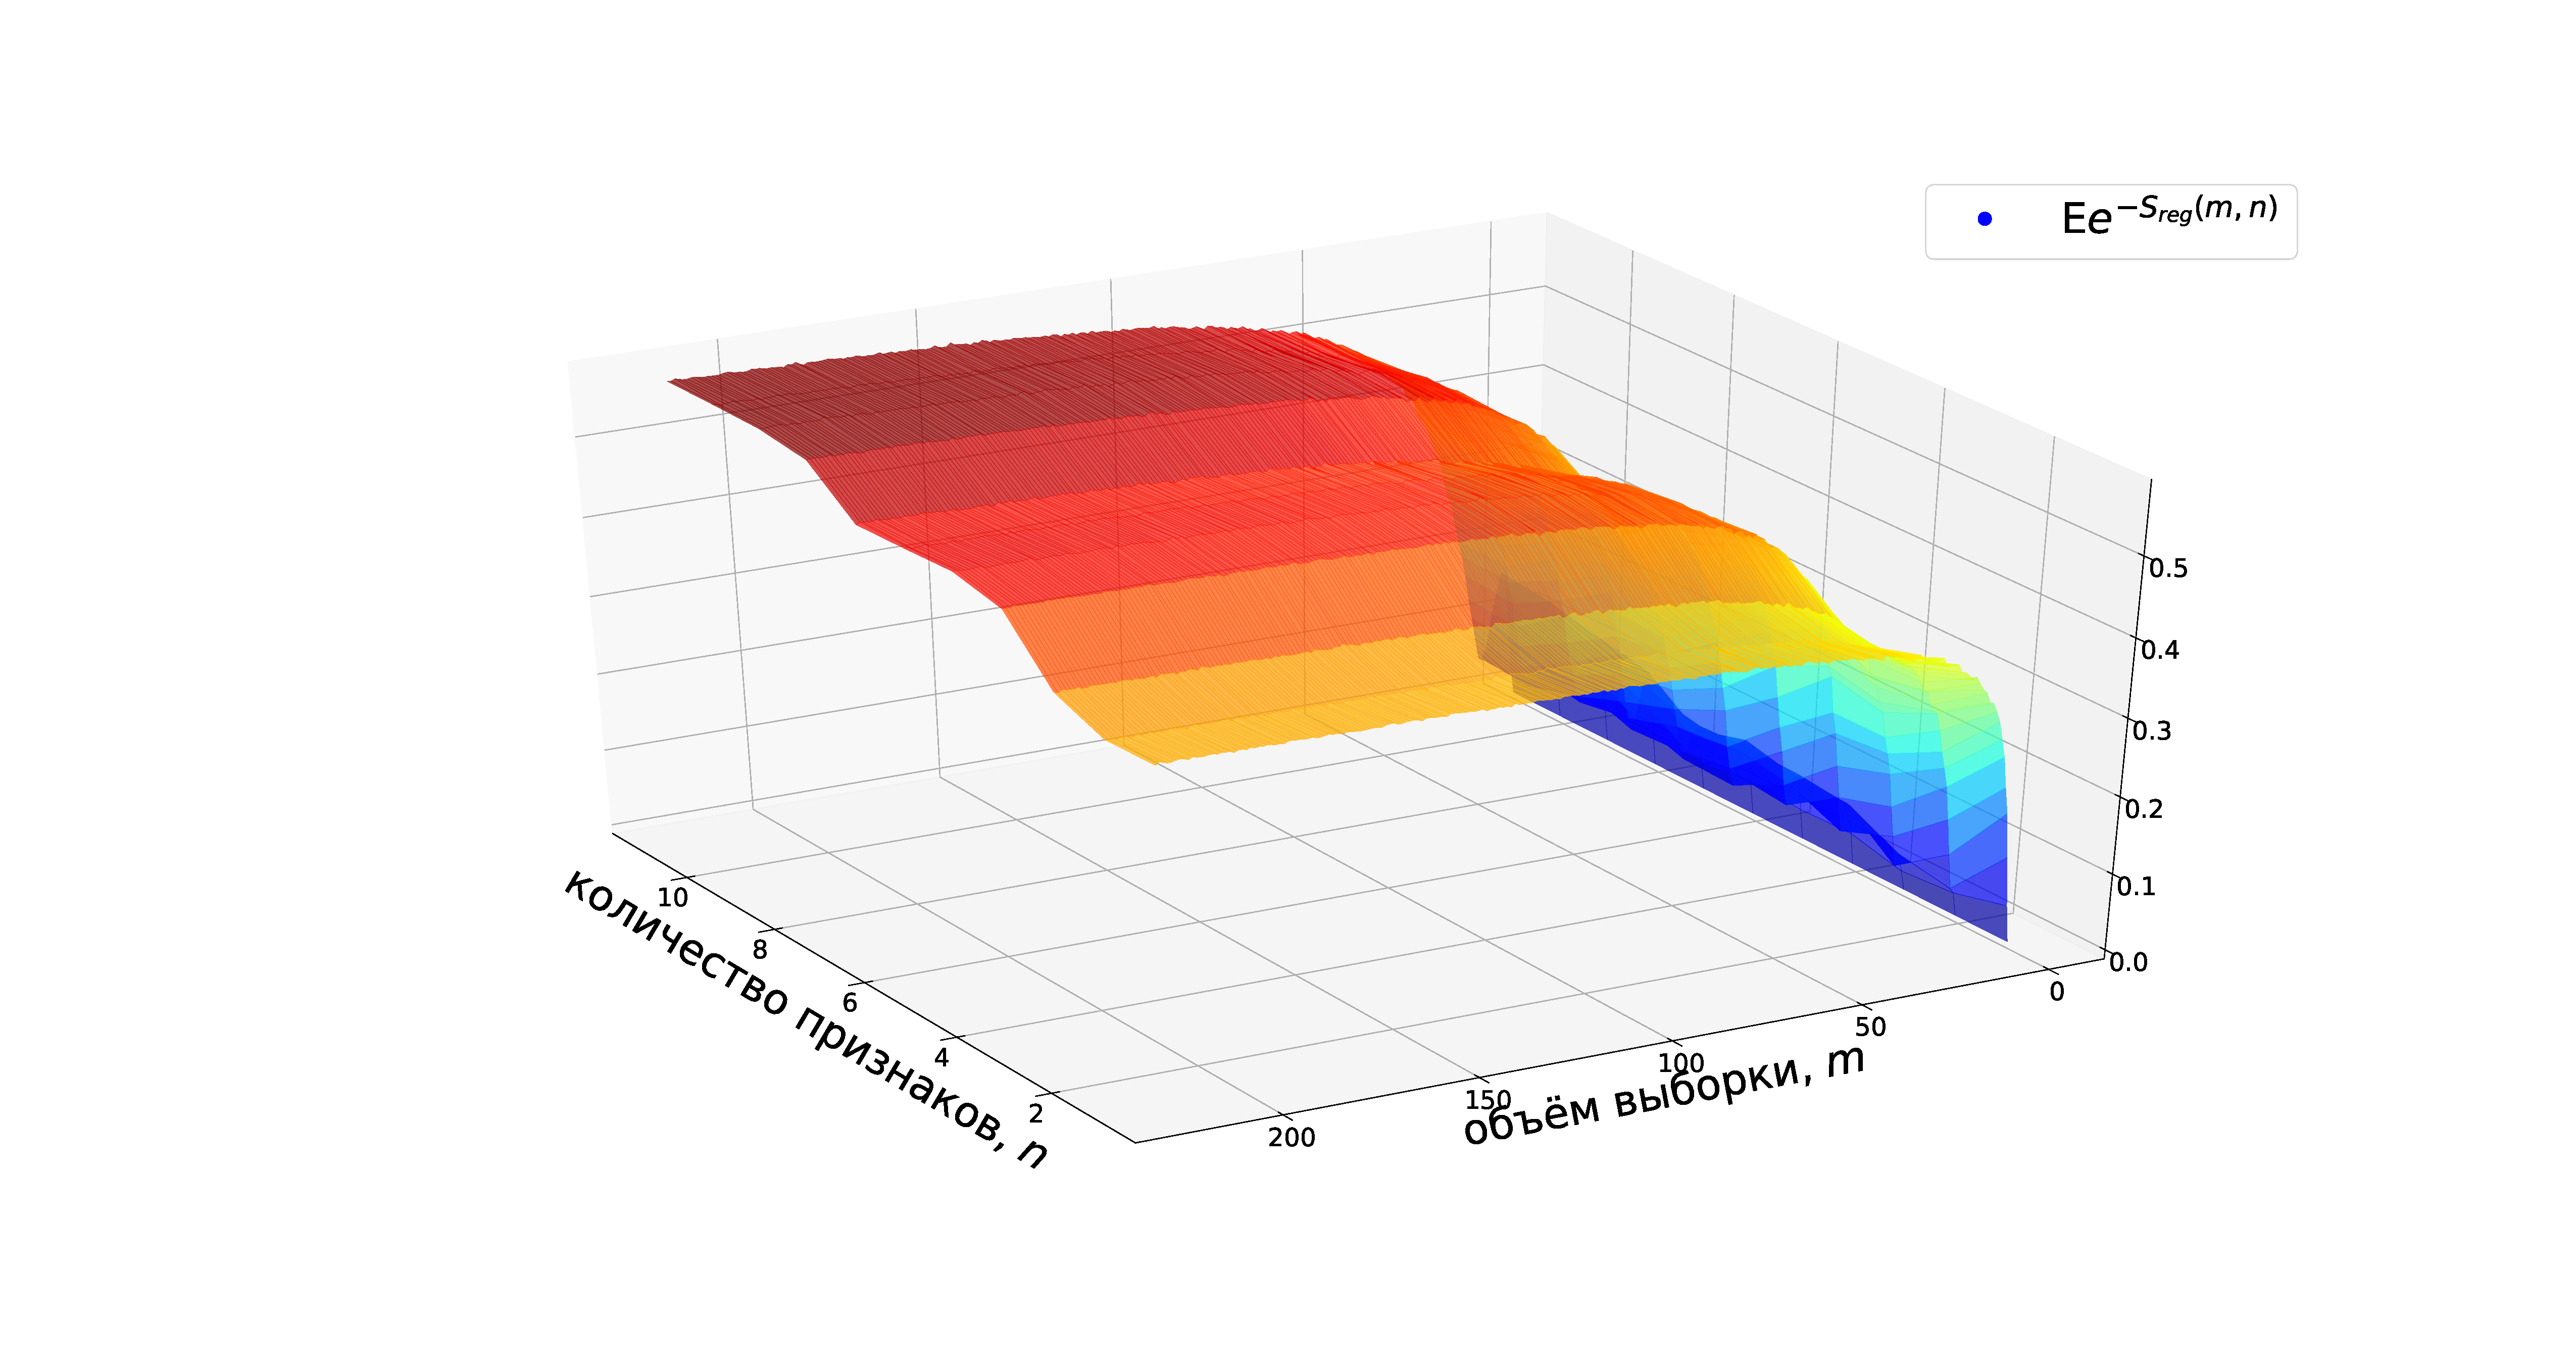
\includegraphics[width=0.5\textwidth]{../data/pics/diabetes_sample_llh.pdf}}&
\subfloat[Diabetes]{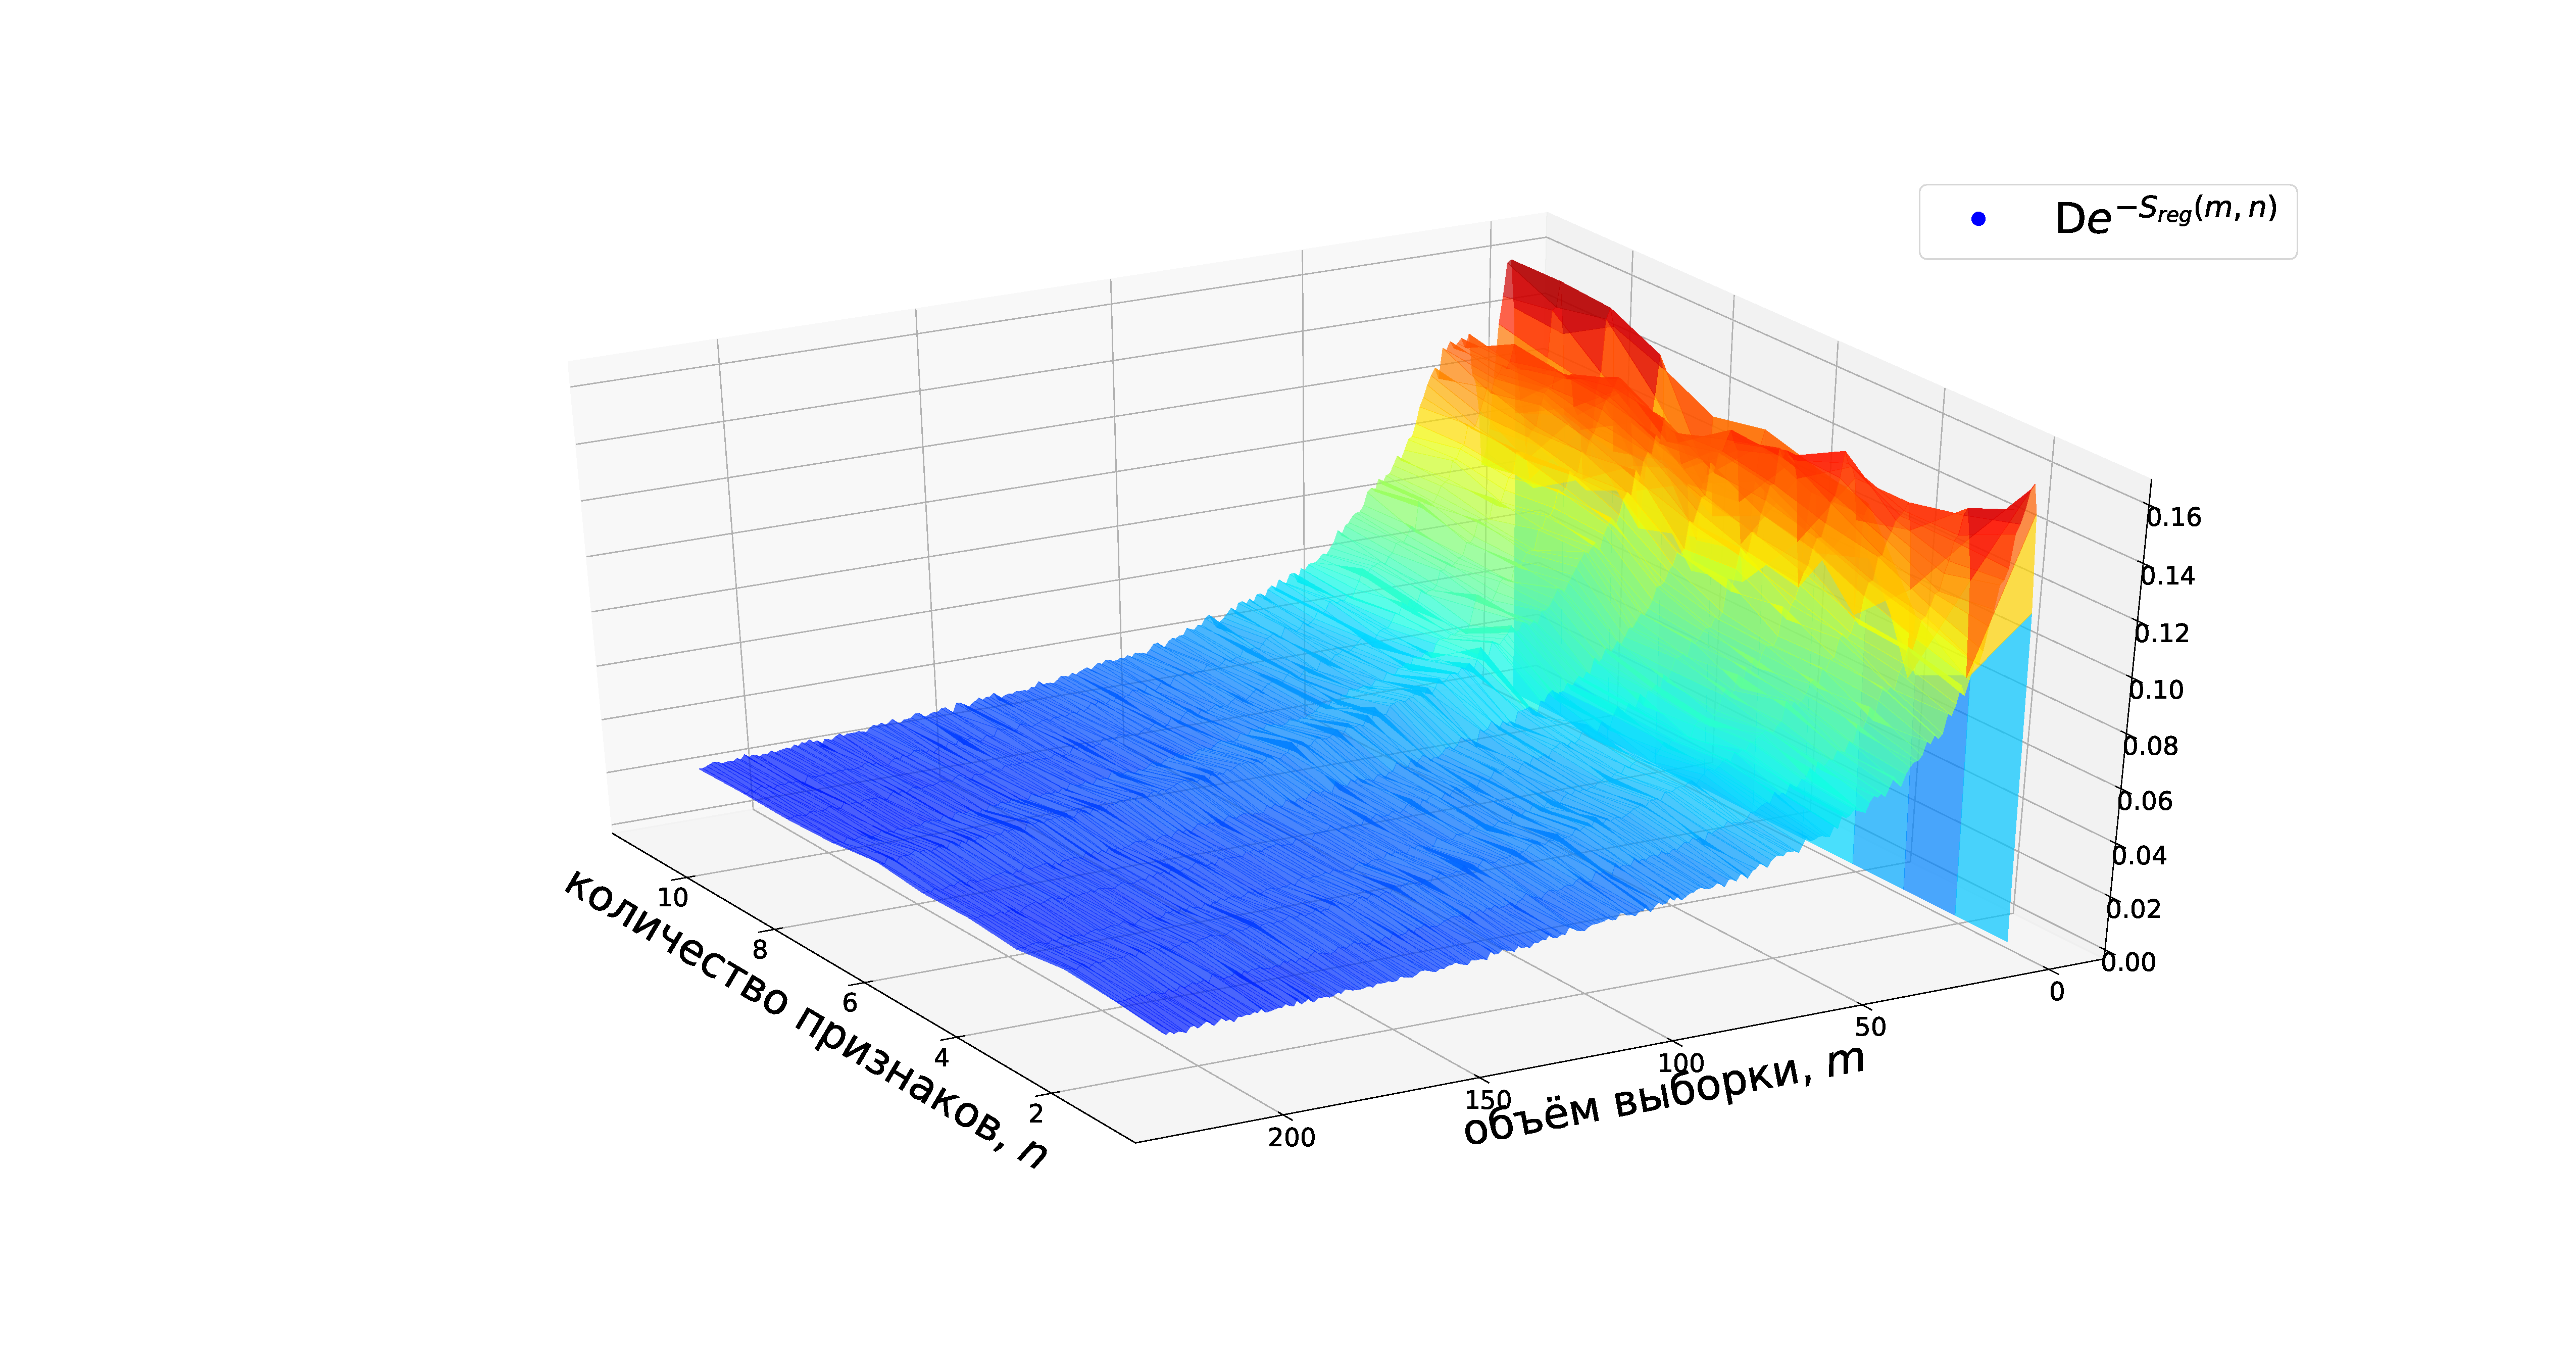
\includegraphics[width=0.5\textwidth]{../data/pics/diabetes_sample_llh_std.pdf}}\\
\subfloat[Boston]{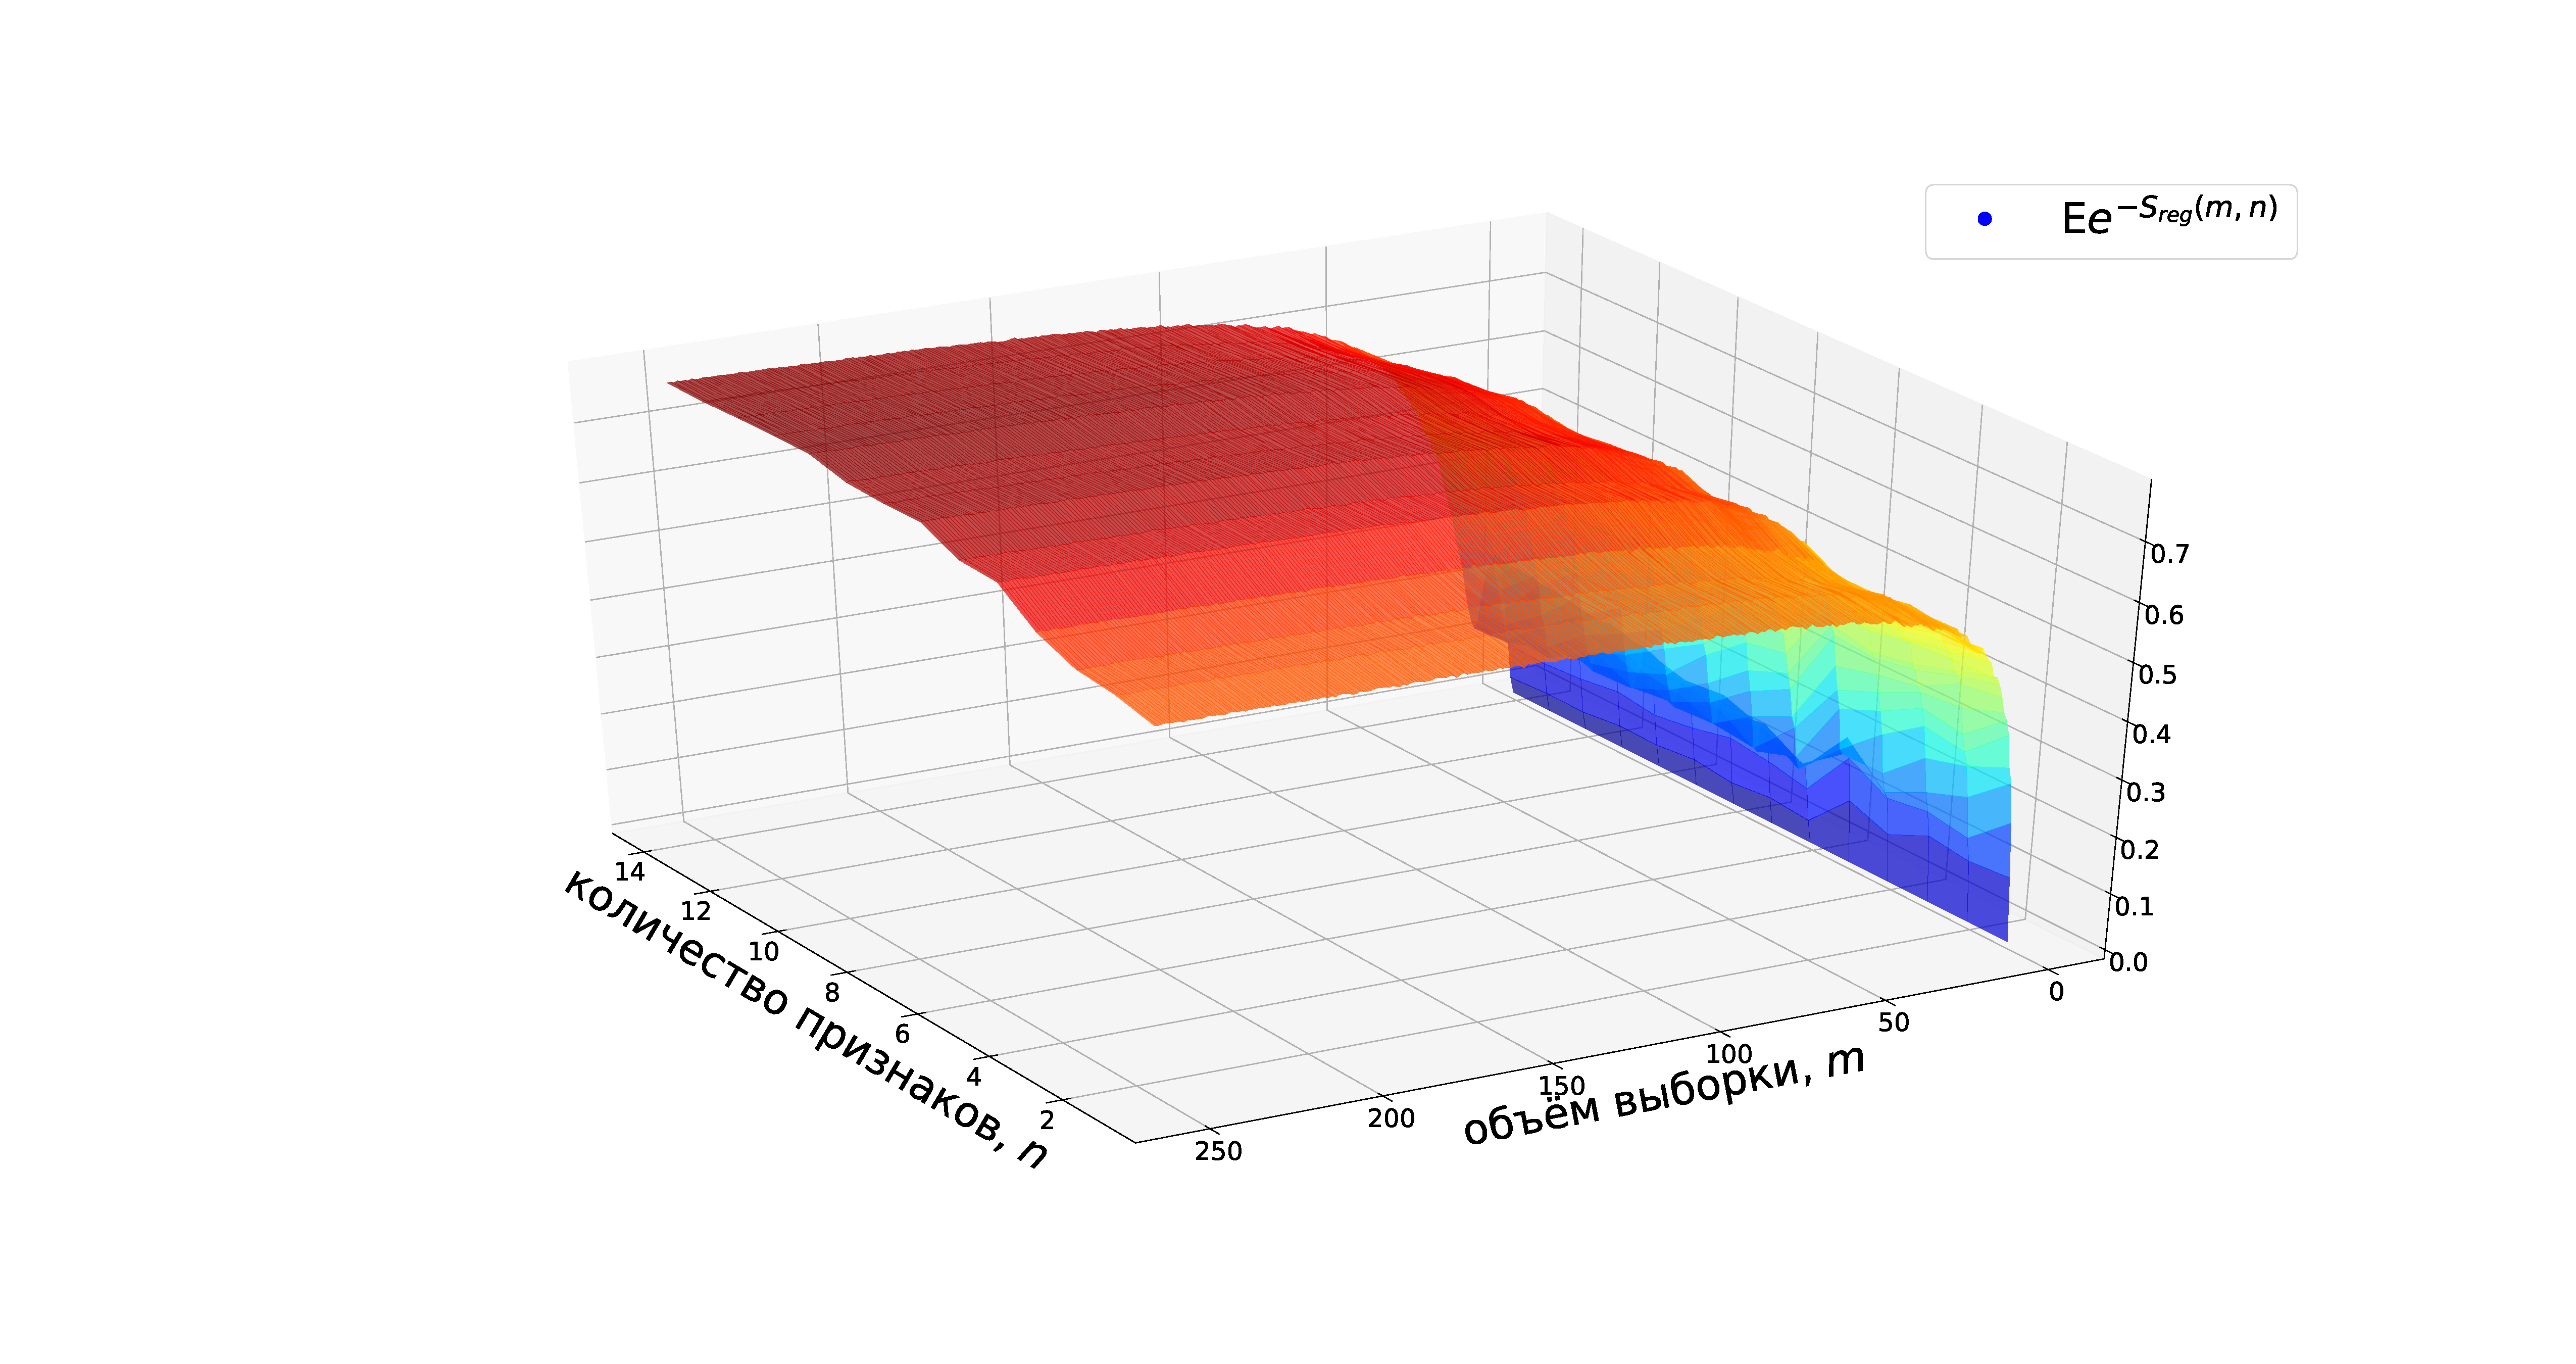
\includegraphics[width=0.5\textwidth]{../data/pics/boston_sample_llh.pdf}}&
\subfloat[Boston]{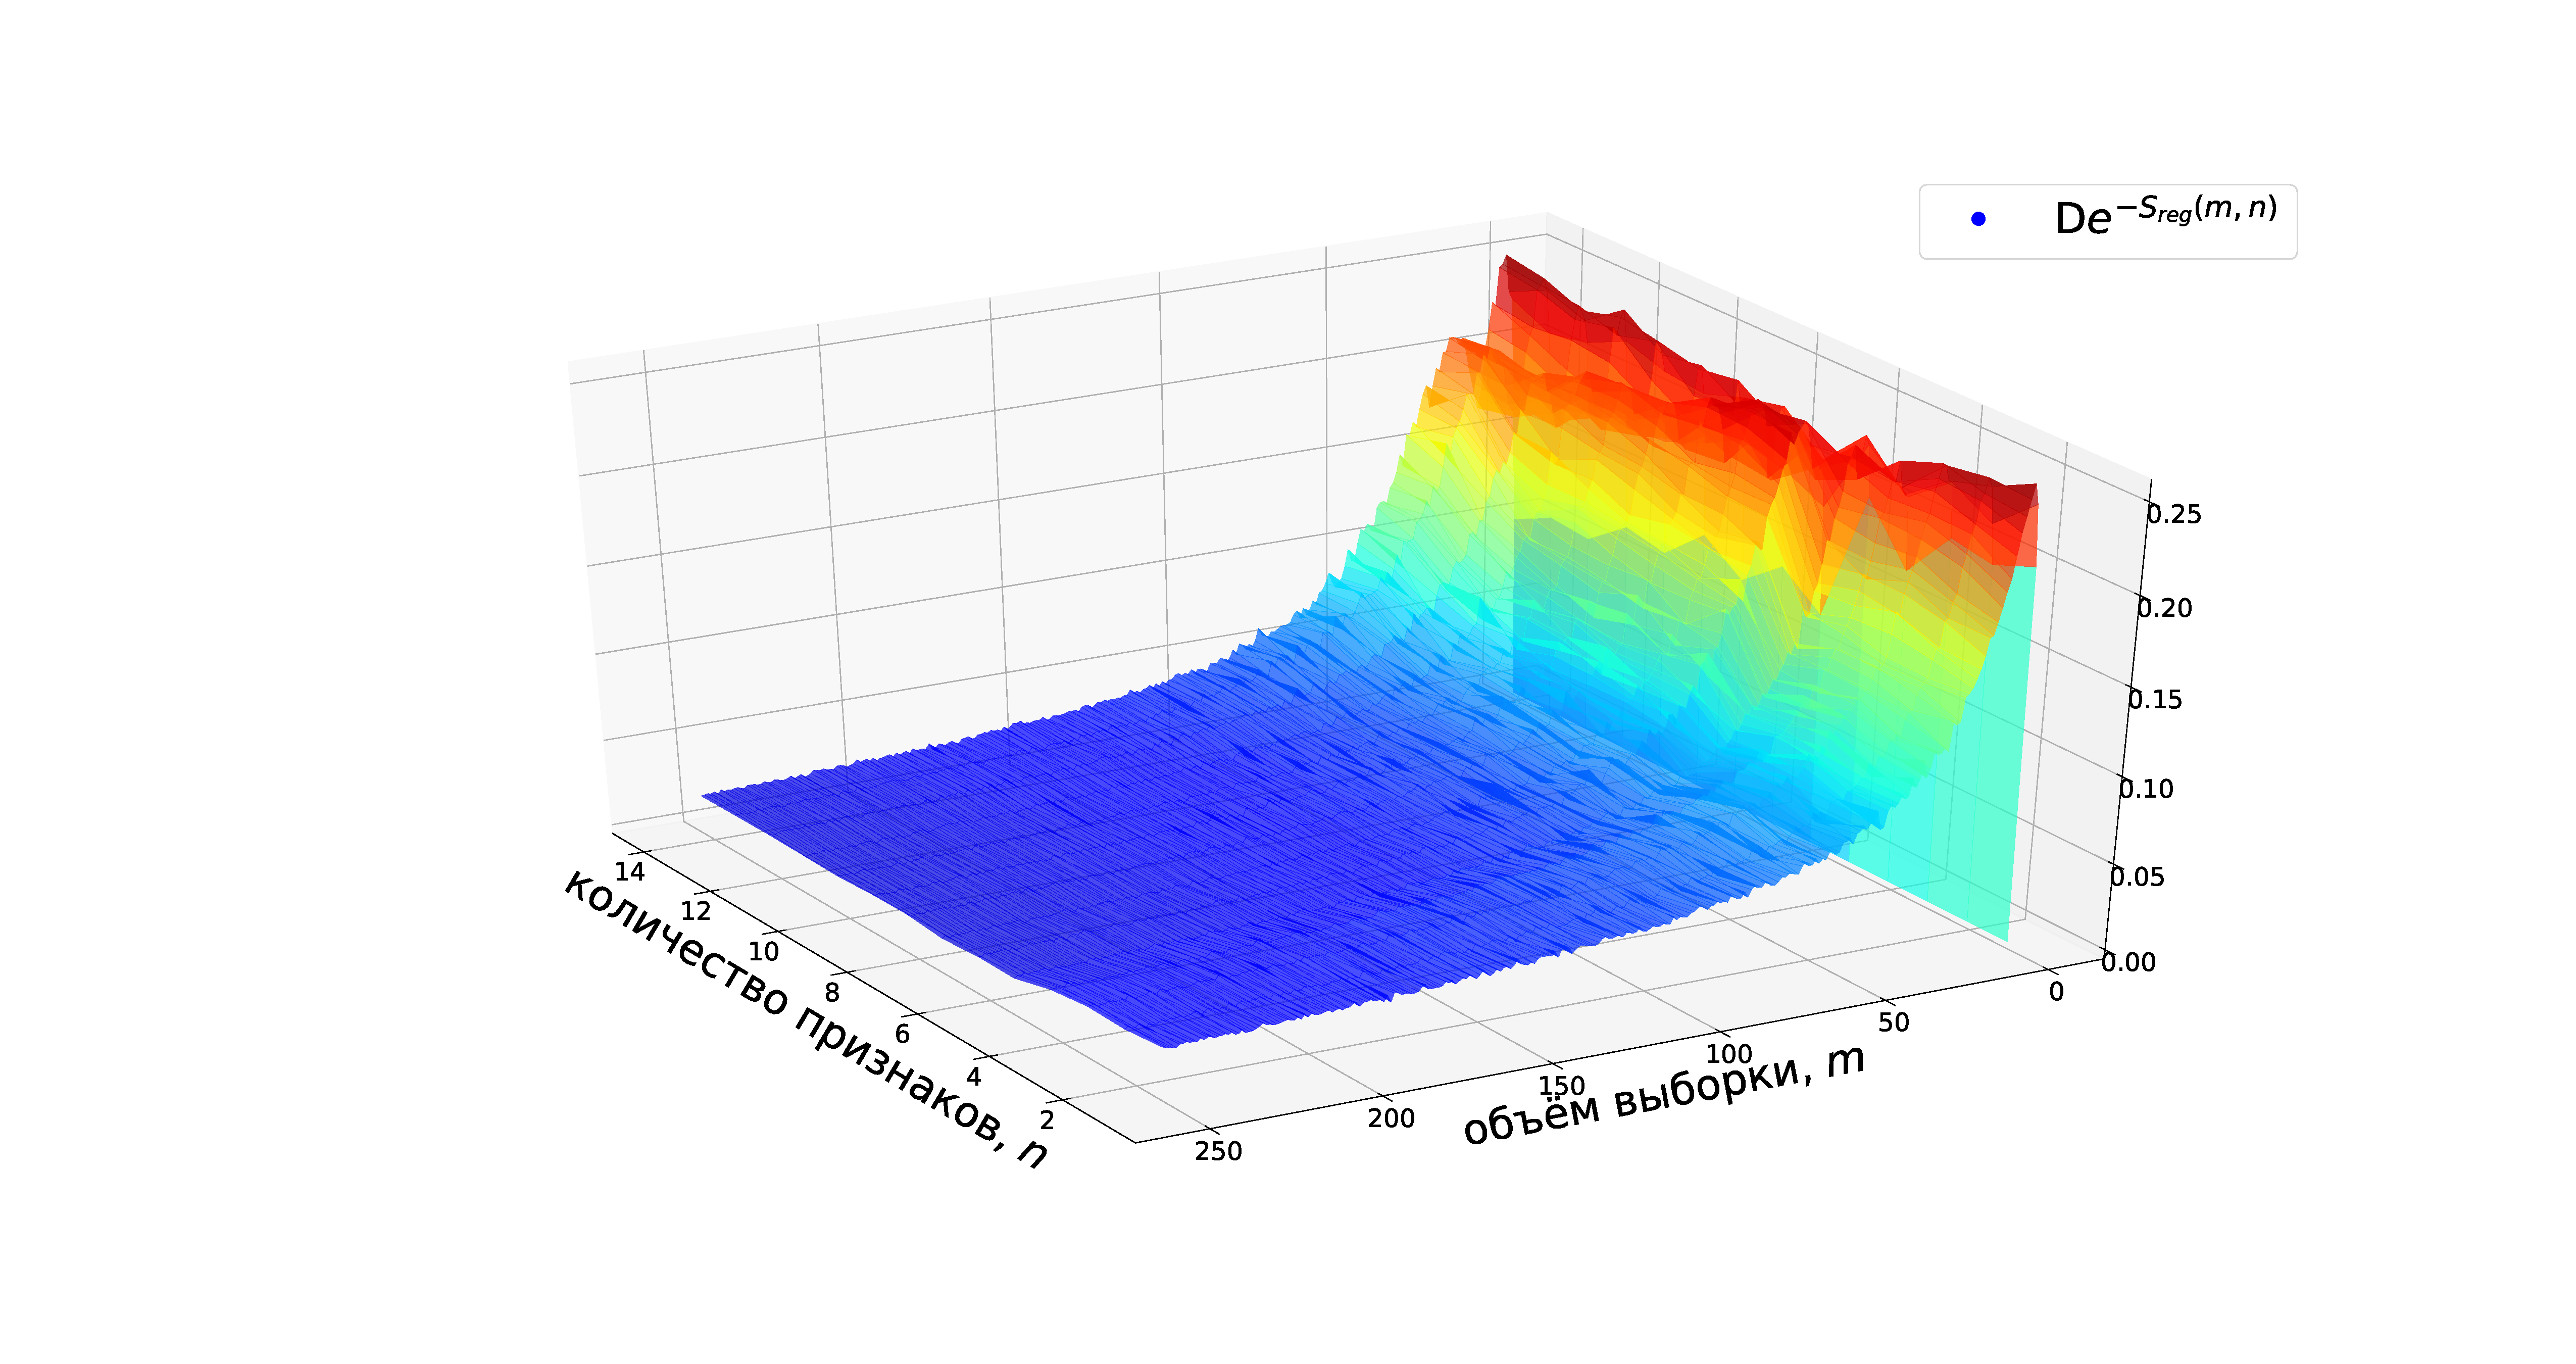
\includegraphics[width=0.5\textwidth]{../data/pics/boston_sample_llh_std.pdf}}\\
\subfloat[Wine]{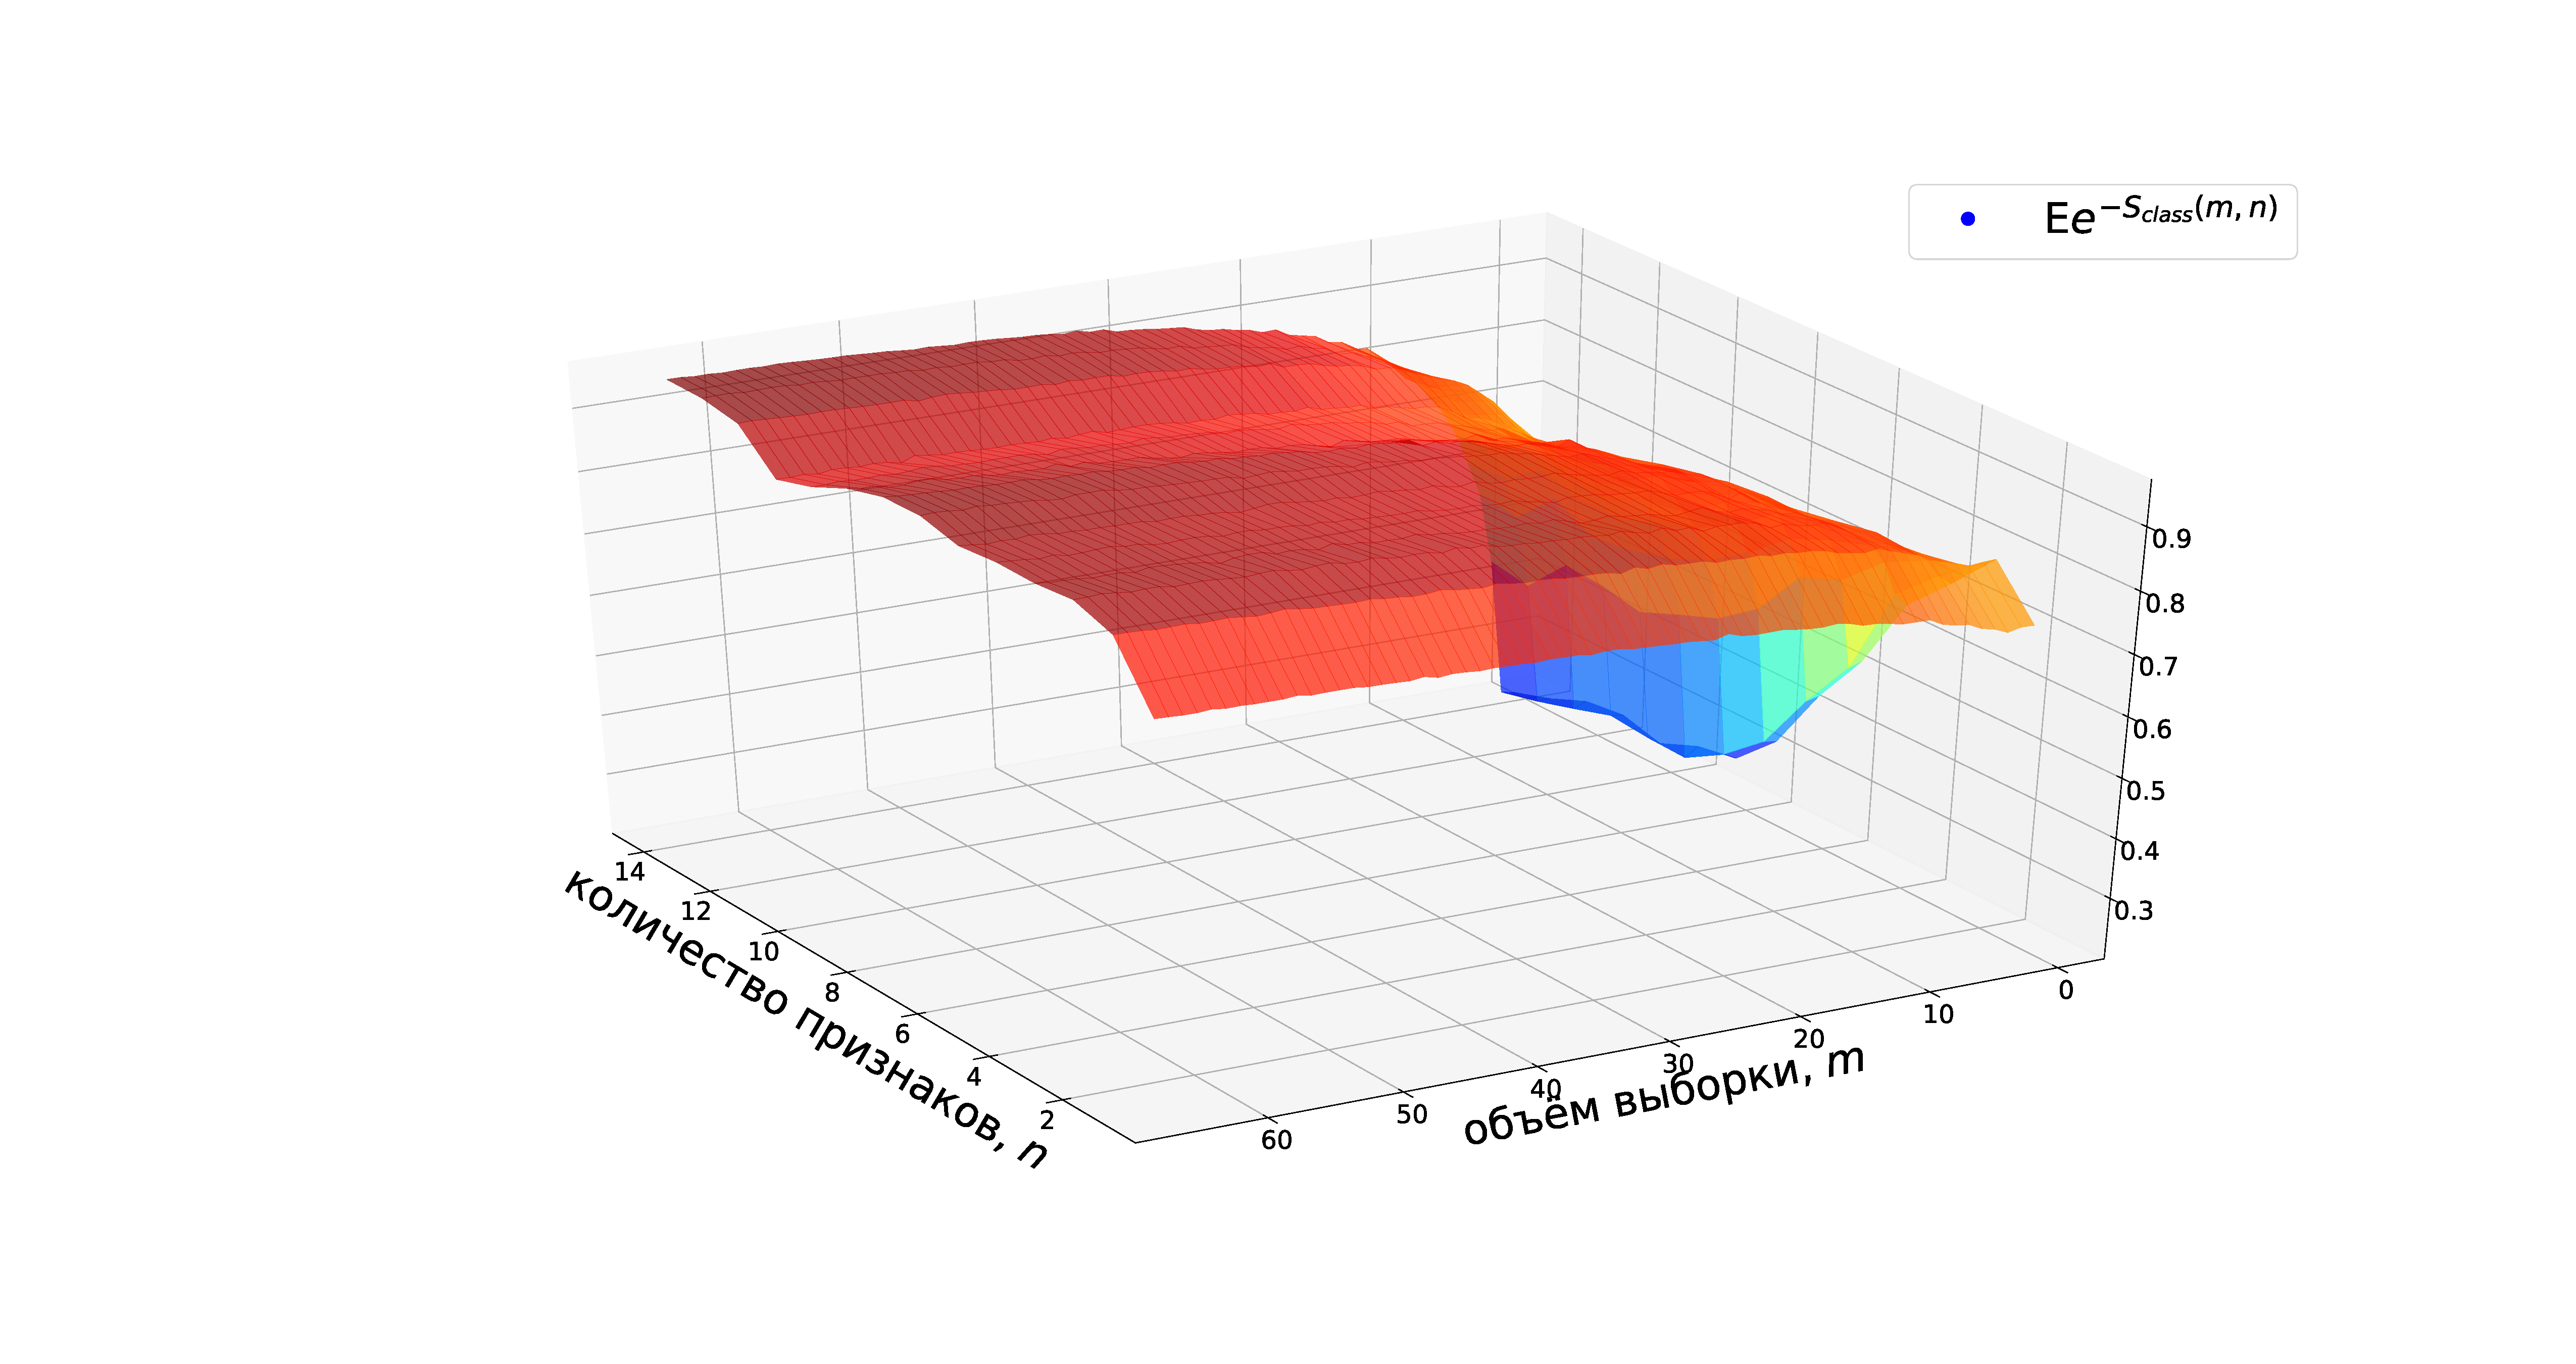
\includegraphics[width=0.5\textwidth]{../data/pics/wine_sample_llh.pdf}}&
\subfloat[Wine]{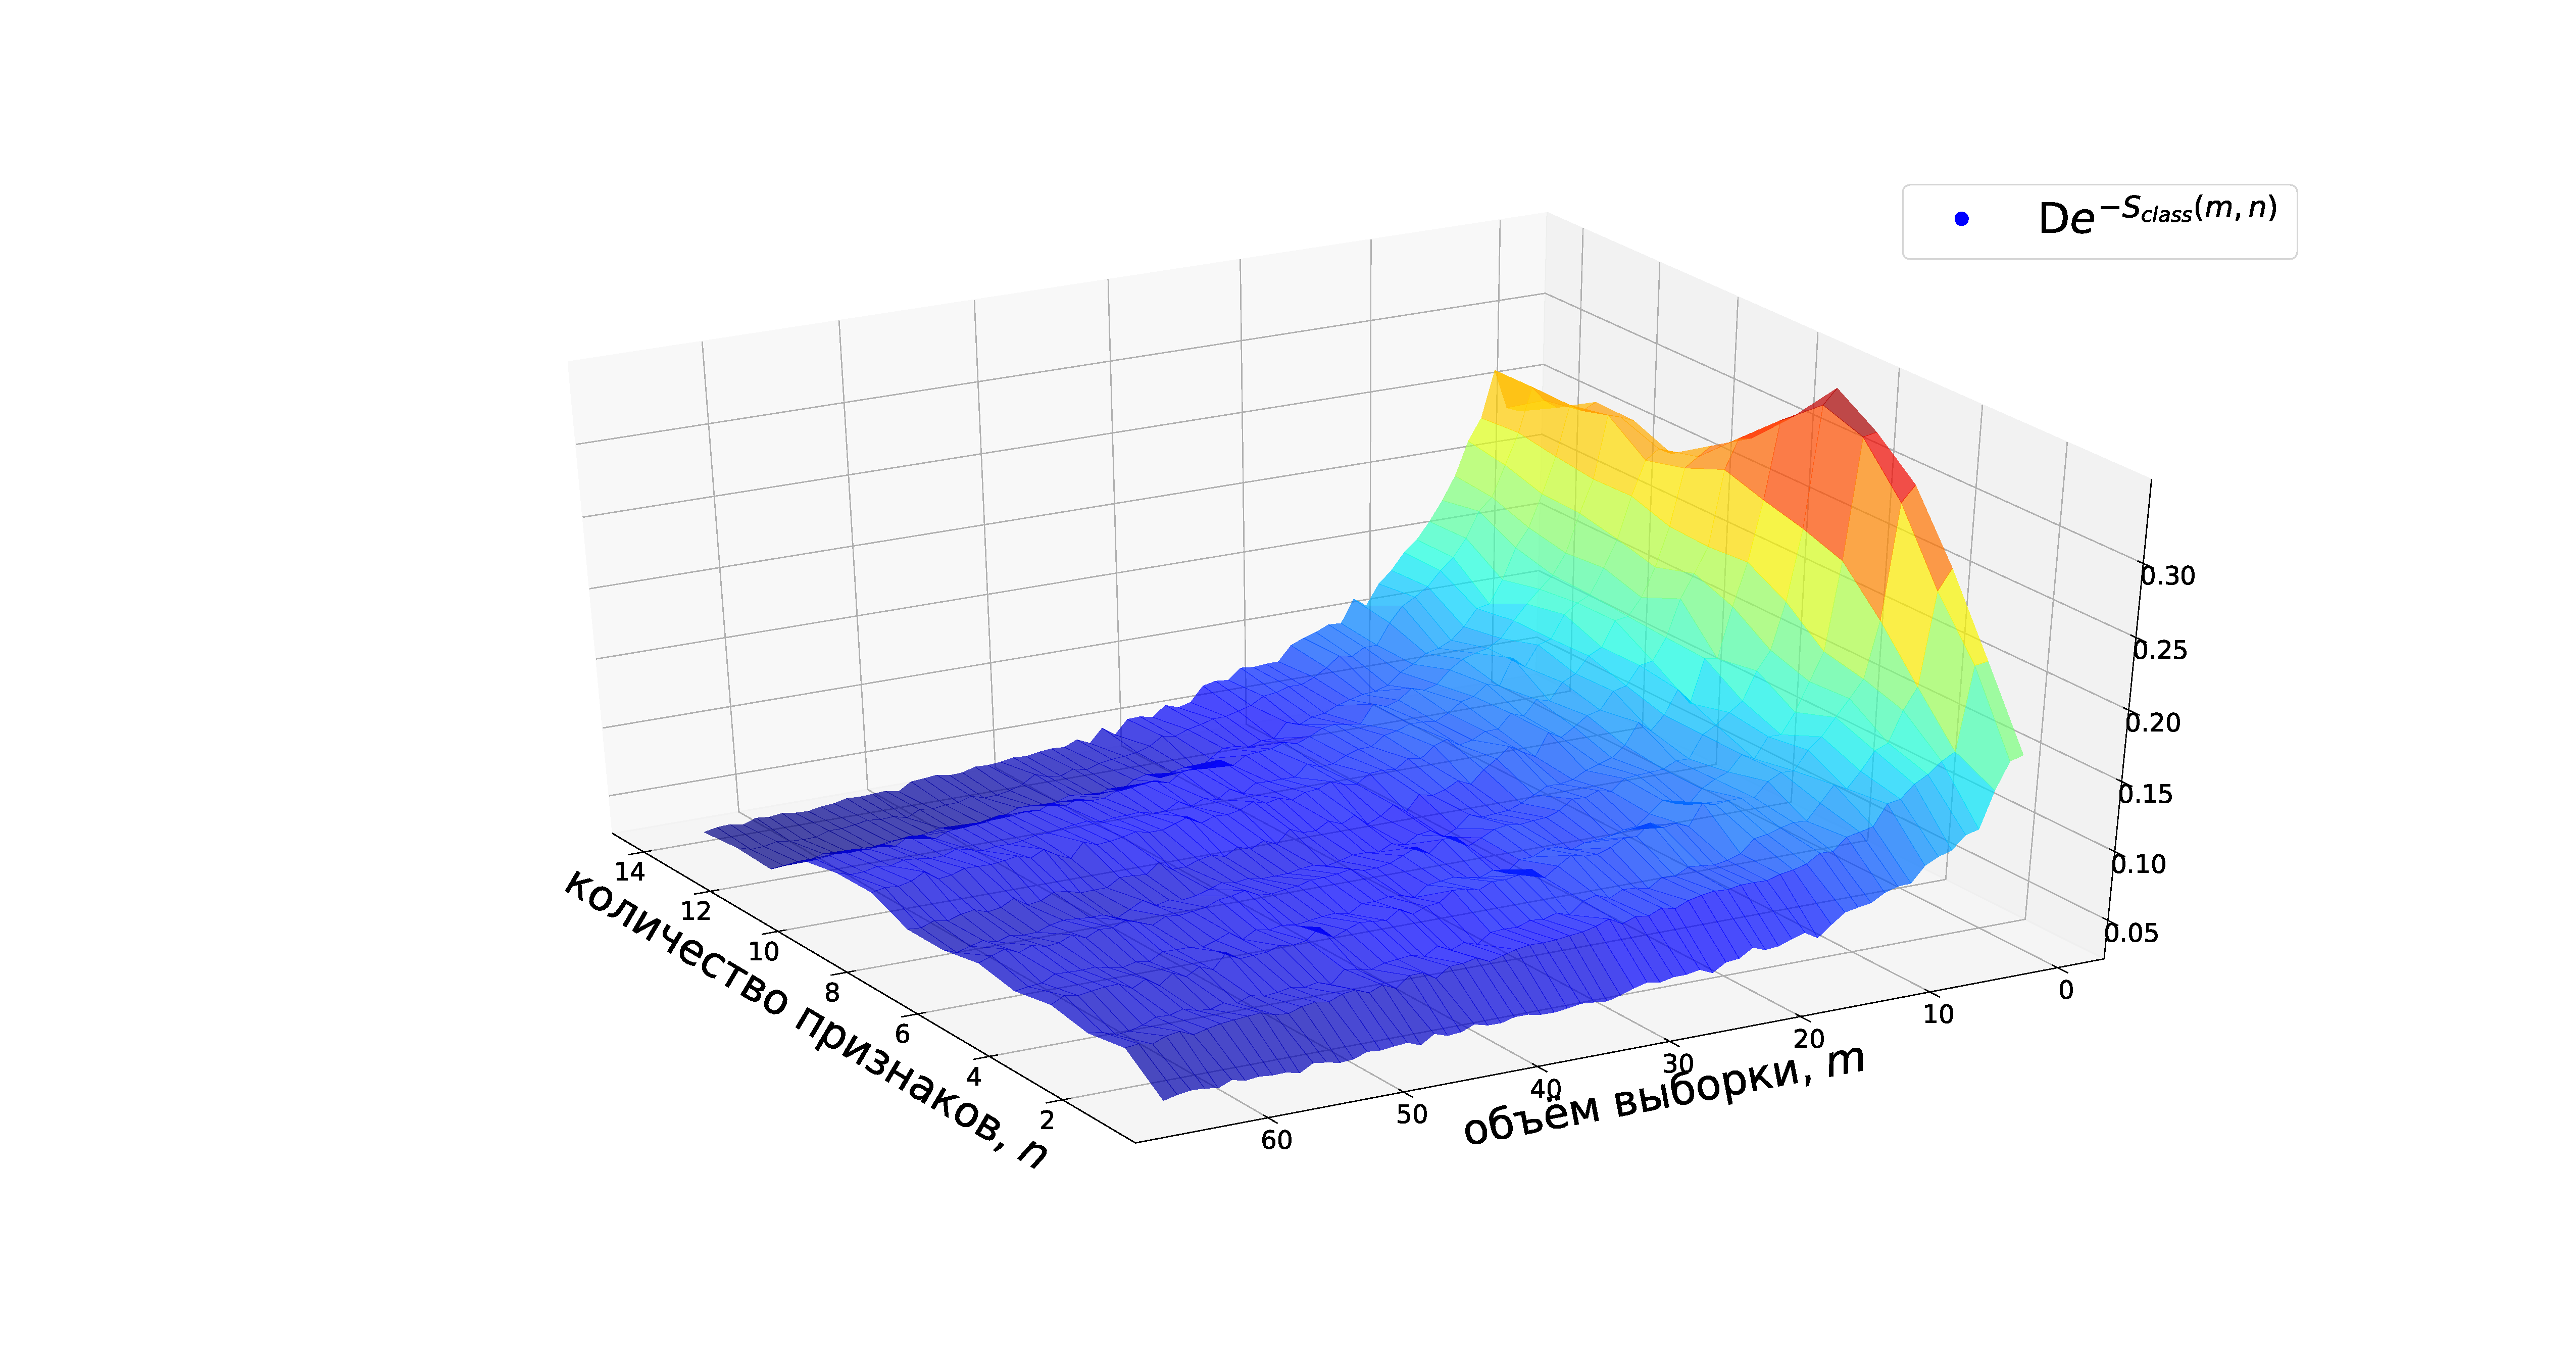
\includegraphics[width=0.5\textwidth]{../data/pics/wine_sample_llh_std.pdf}}\\
\subfloat[Nba]{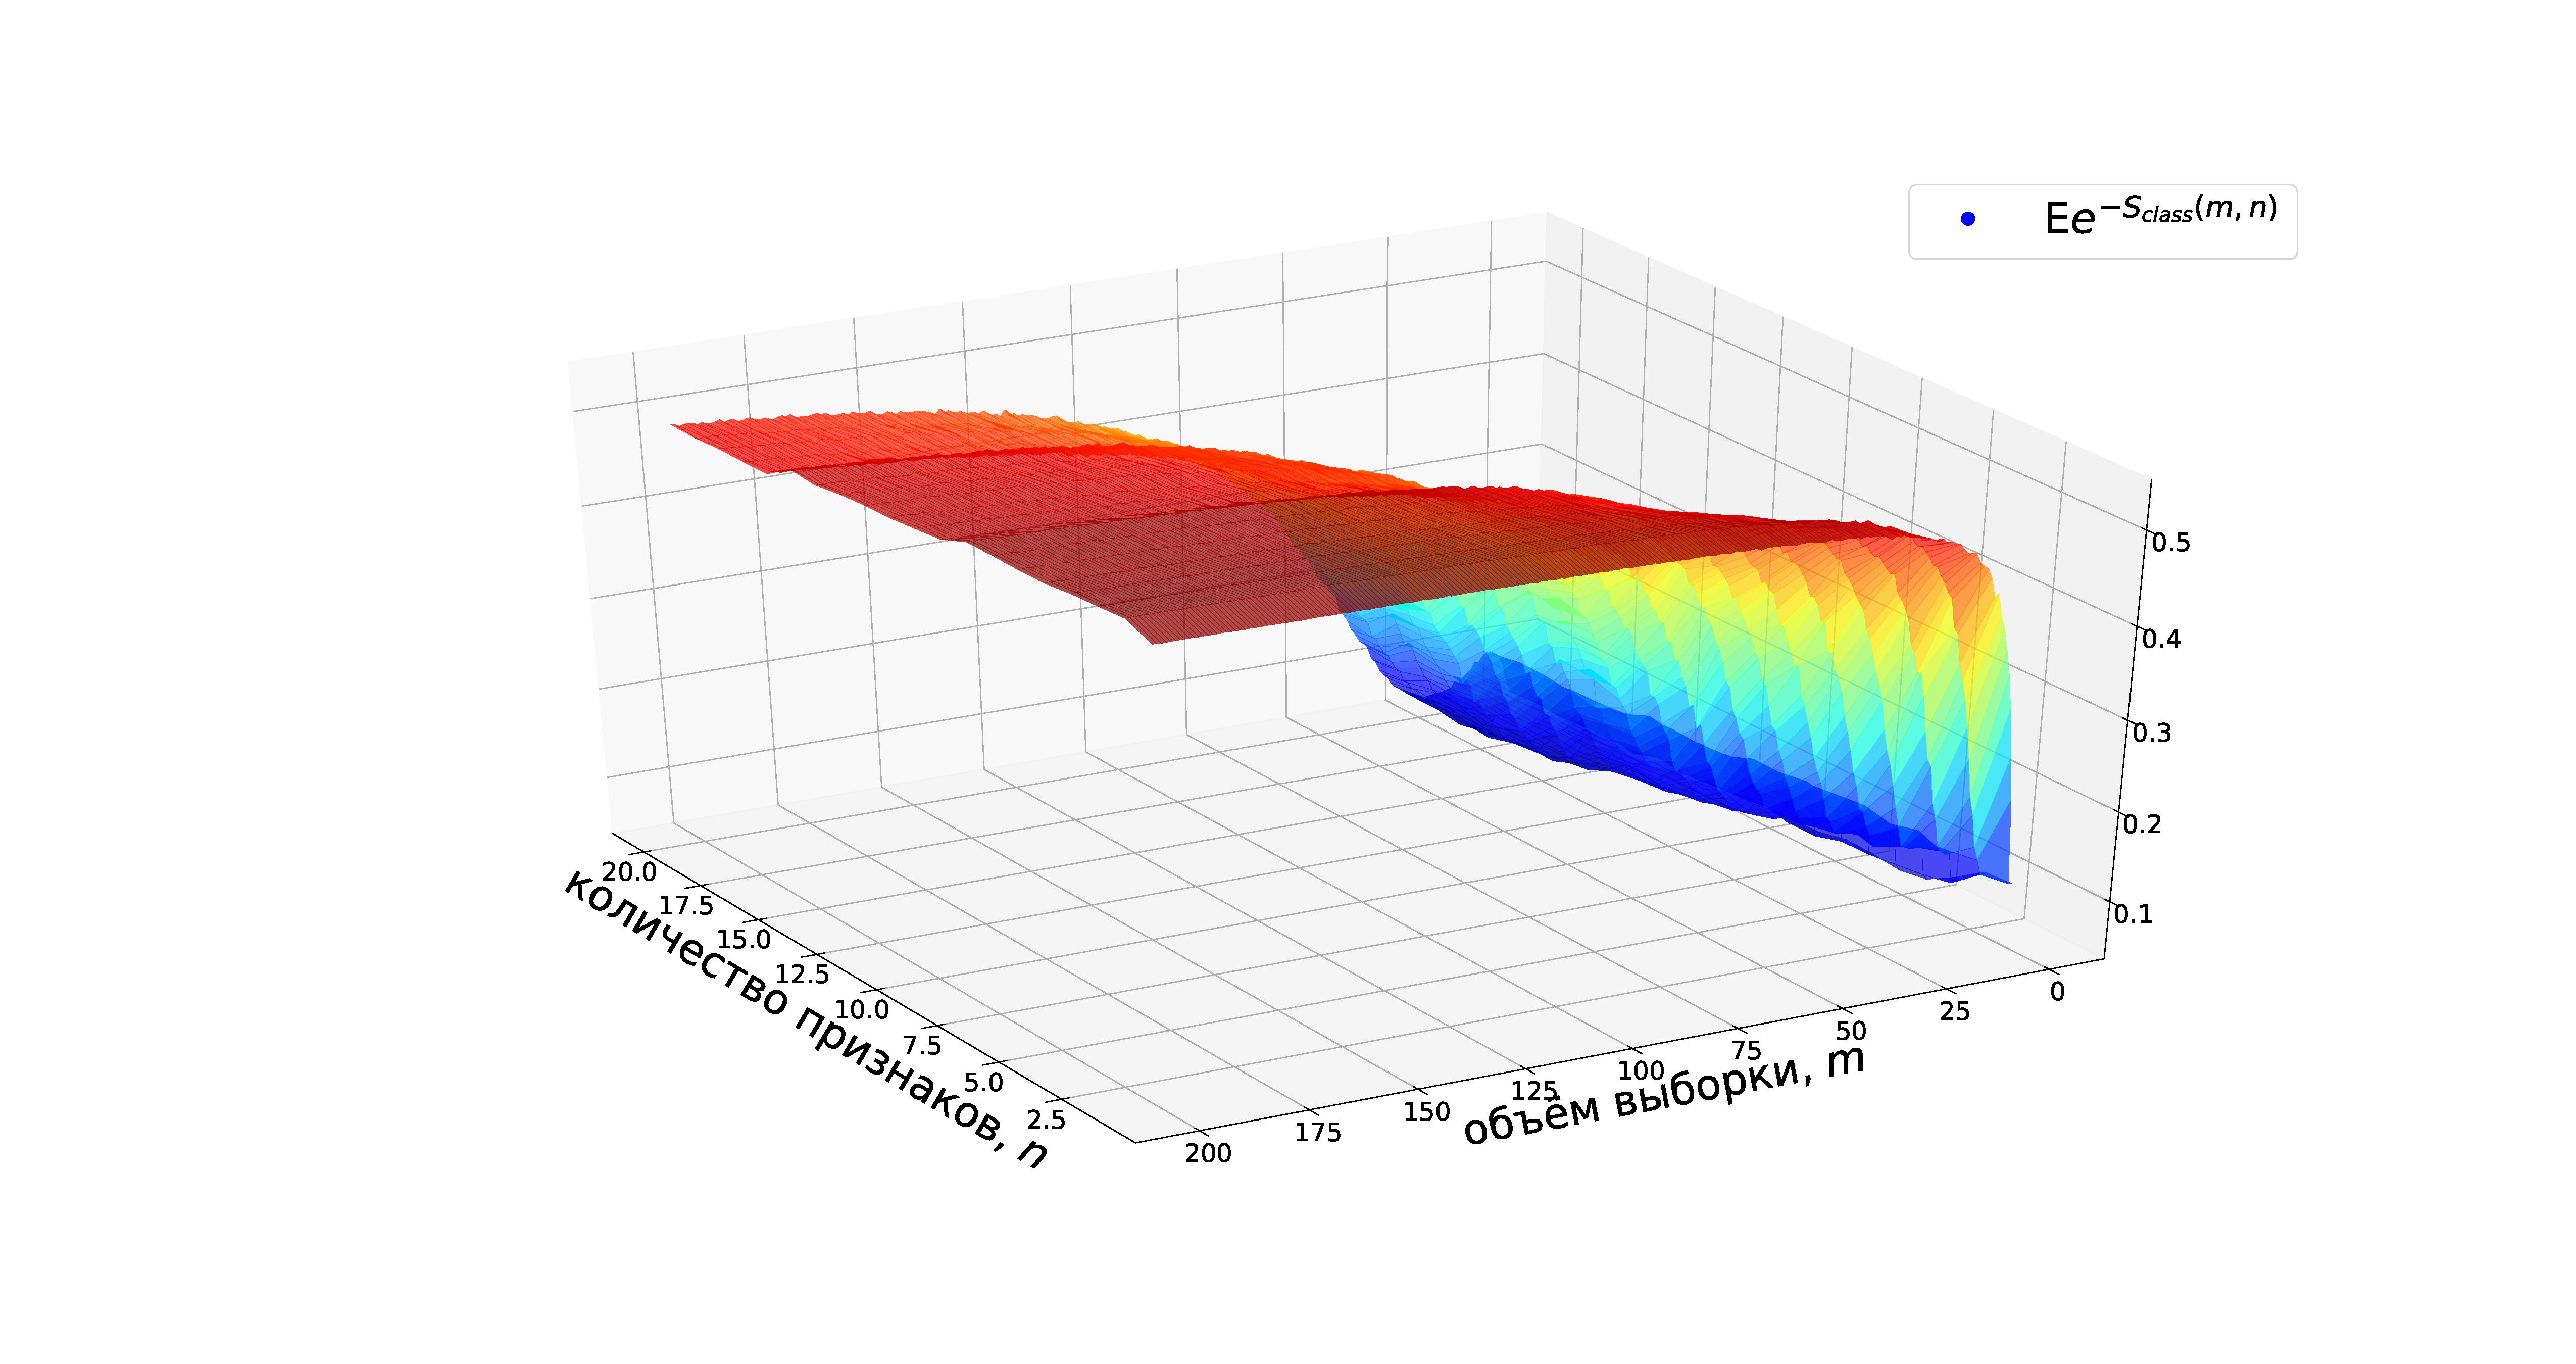
\includegraphics[width=0.5\textwidth]{../data/pics/nba_sample_llh.pdf}}&
\subfloat[Nba]{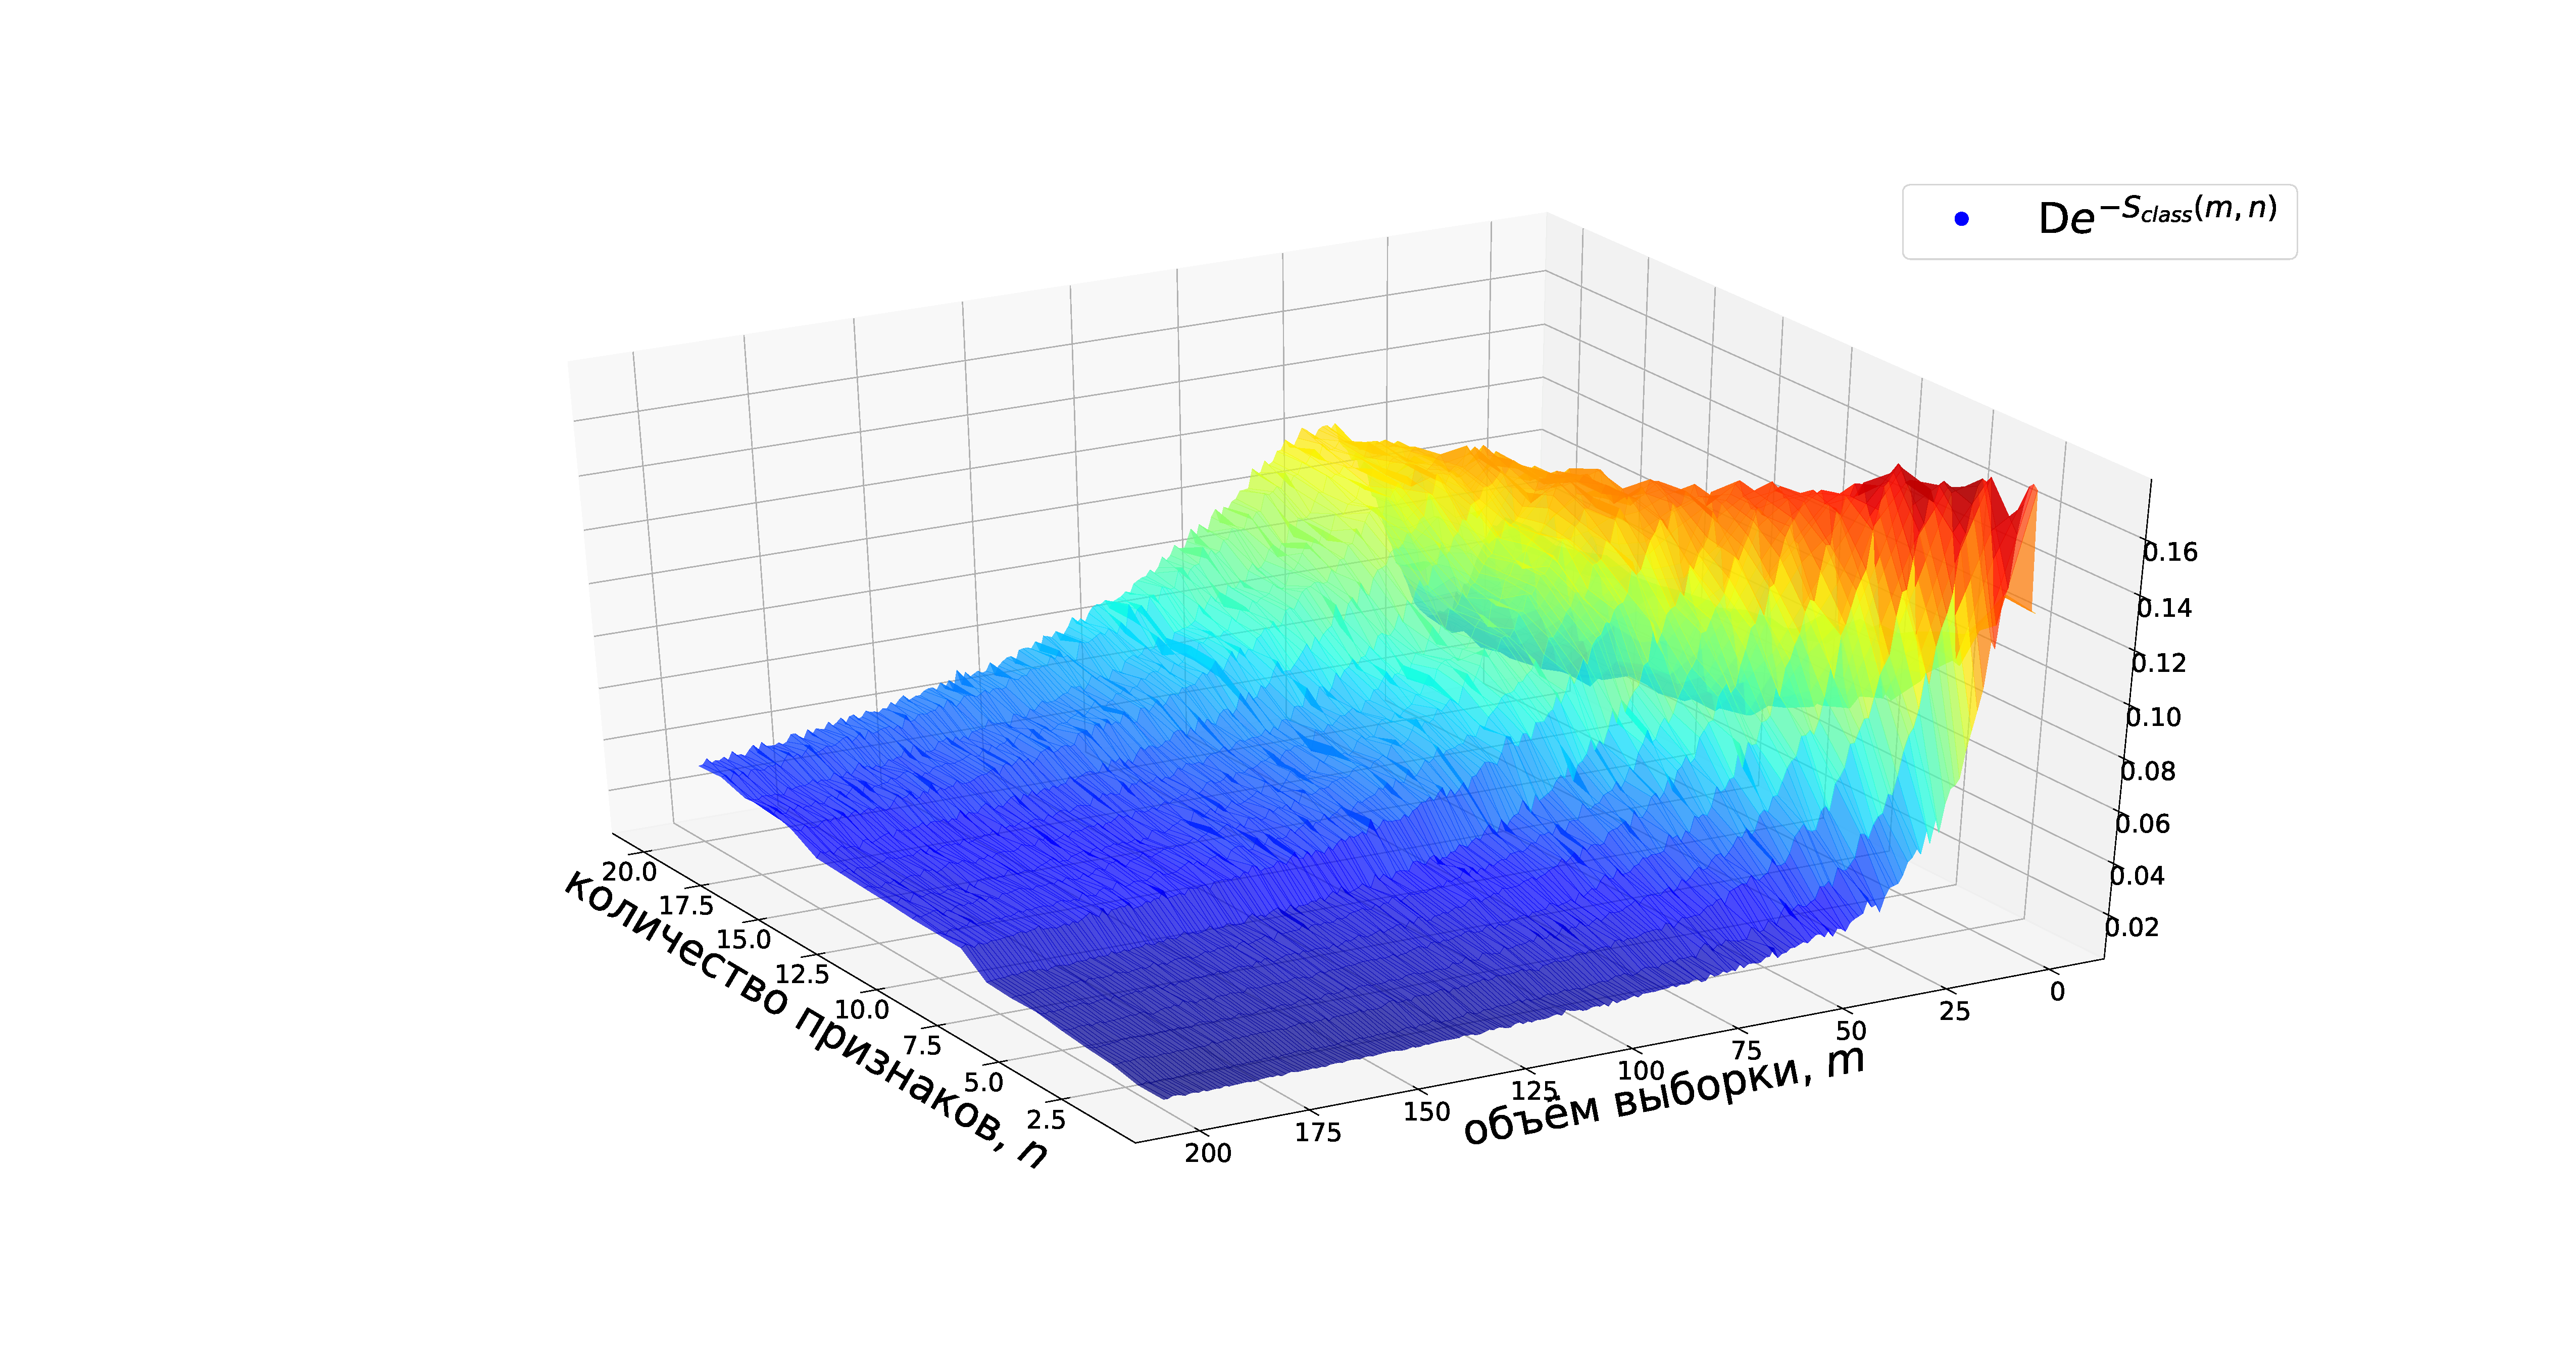
\includegraphics[width=0.5\textwidth]{../data/pics/nba_sample_llh_std.pdf}}\\
\end{tabular}

\caption{Зависимость значения функции $e^{-S(m, n)}$ от объема выборки $m$ и количества параметров $n$ для выборок из UCI репозитория}
\label{fig3}
\end{figure}

На рис. 4. представлены графики качества аппроксимации функции $\hat{l}(m)$, а также предсказание $\hat{m^*}$ при различных $m_0$ для разных выборок. Так же, как и для синтетических выборок, аппроксимация функции $\hat{l}(m)$ в варианте с неполной информацией даёт качество хуже, чем в варианте с полной информацией. Также качество аппроксимации в варианте с неполной информацией сильно шумит при малых значениях $m_0$.

При $m_0 \rightarrow m$ аппроксимация в варианте с неполной информацией стремится к аппроксимации в варианте с полной информацией, поэтому при больших $m_0$ предсказания $\hat{m^*}$ для этих двух вариантов практически совпадают.

Для выборок задачи регрессии получилось построить адекватное предсказание достаточного объёма выборки $\hat{m^*}$ при $m_0 < m^*$.

Для выборок задачи классификации при $m_0 < m^*$ построить адекватное предсказание $\hat{m^*}$ не получилось. Это может быть связано с тем, что достаточный объём $m^*$ для задачи классификации сильно меньше, чем для задачи регрессии, а при меньших $m_0$ аппроксимация функции $\hat{l}(m)$ хуже, чем при больших $m_0$.

\newpage

\begin{figure}[h!t]\center
\centering\begin{tabular}{@{}c@{ }c@{ }c@{}}
\textbf{Аппроксимация $e^{-S(m, n)}$} & \textbf{Предсказание $m^*$}\\
\subfloat[Diabetees]{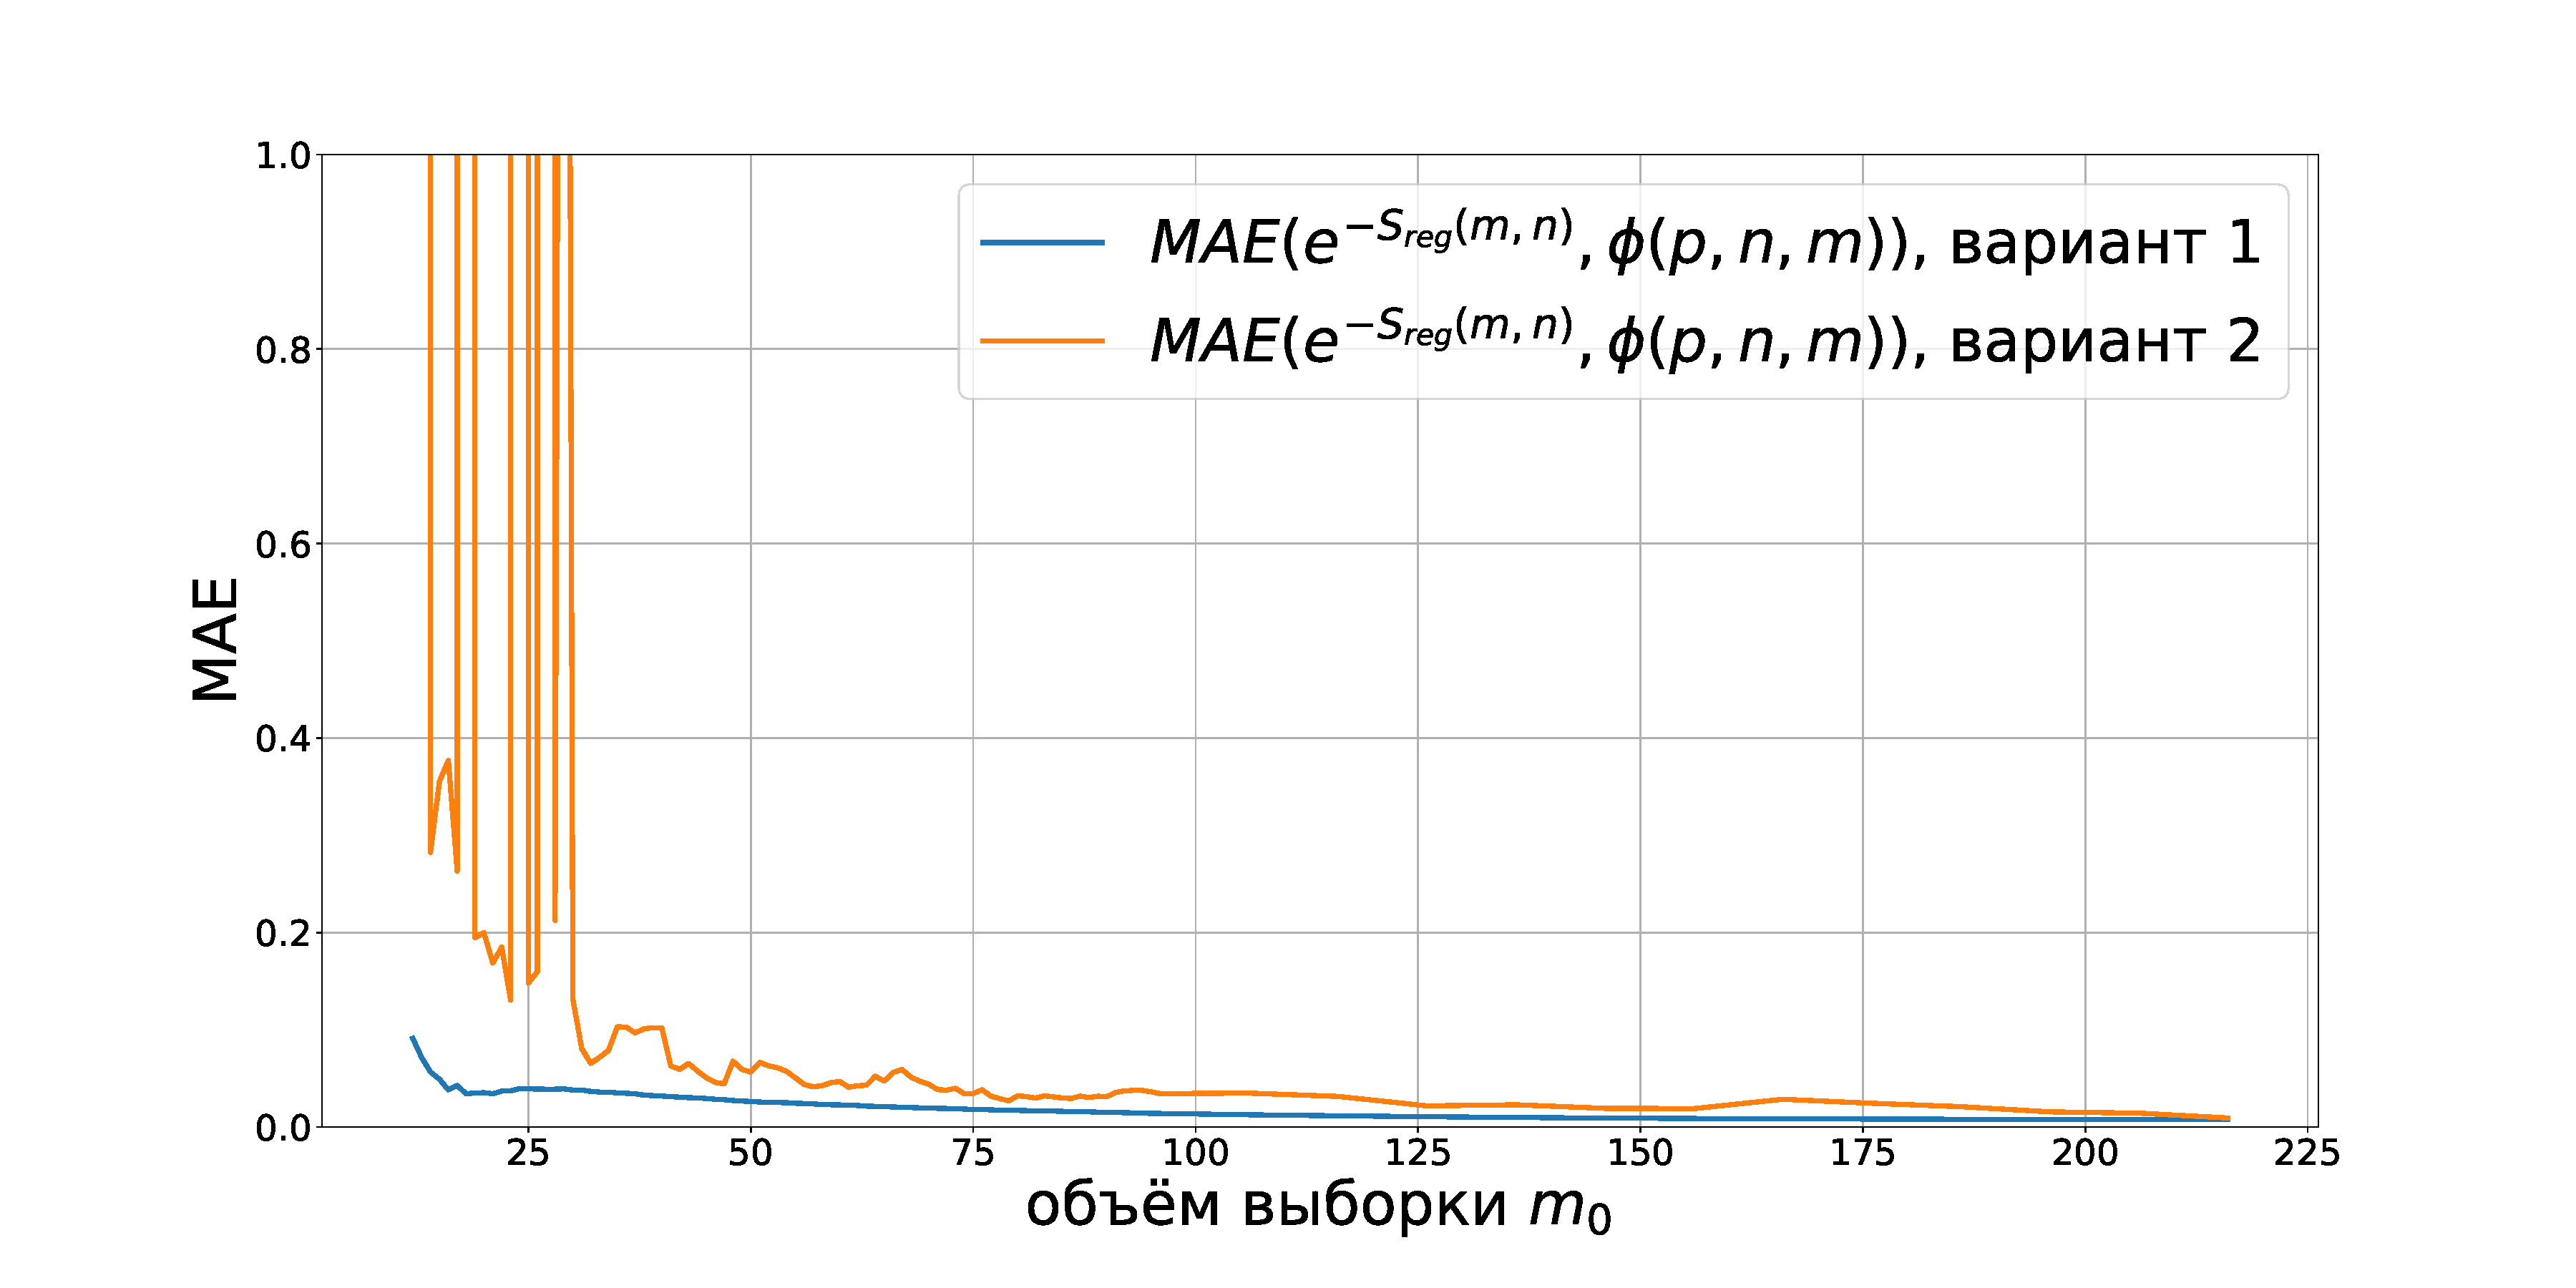
\includegraphics[width=0.5\textwidth]{../data/pics/diabetes_sample_MAPE_comparison.pdf}}&
\subfloat[Diabetees]{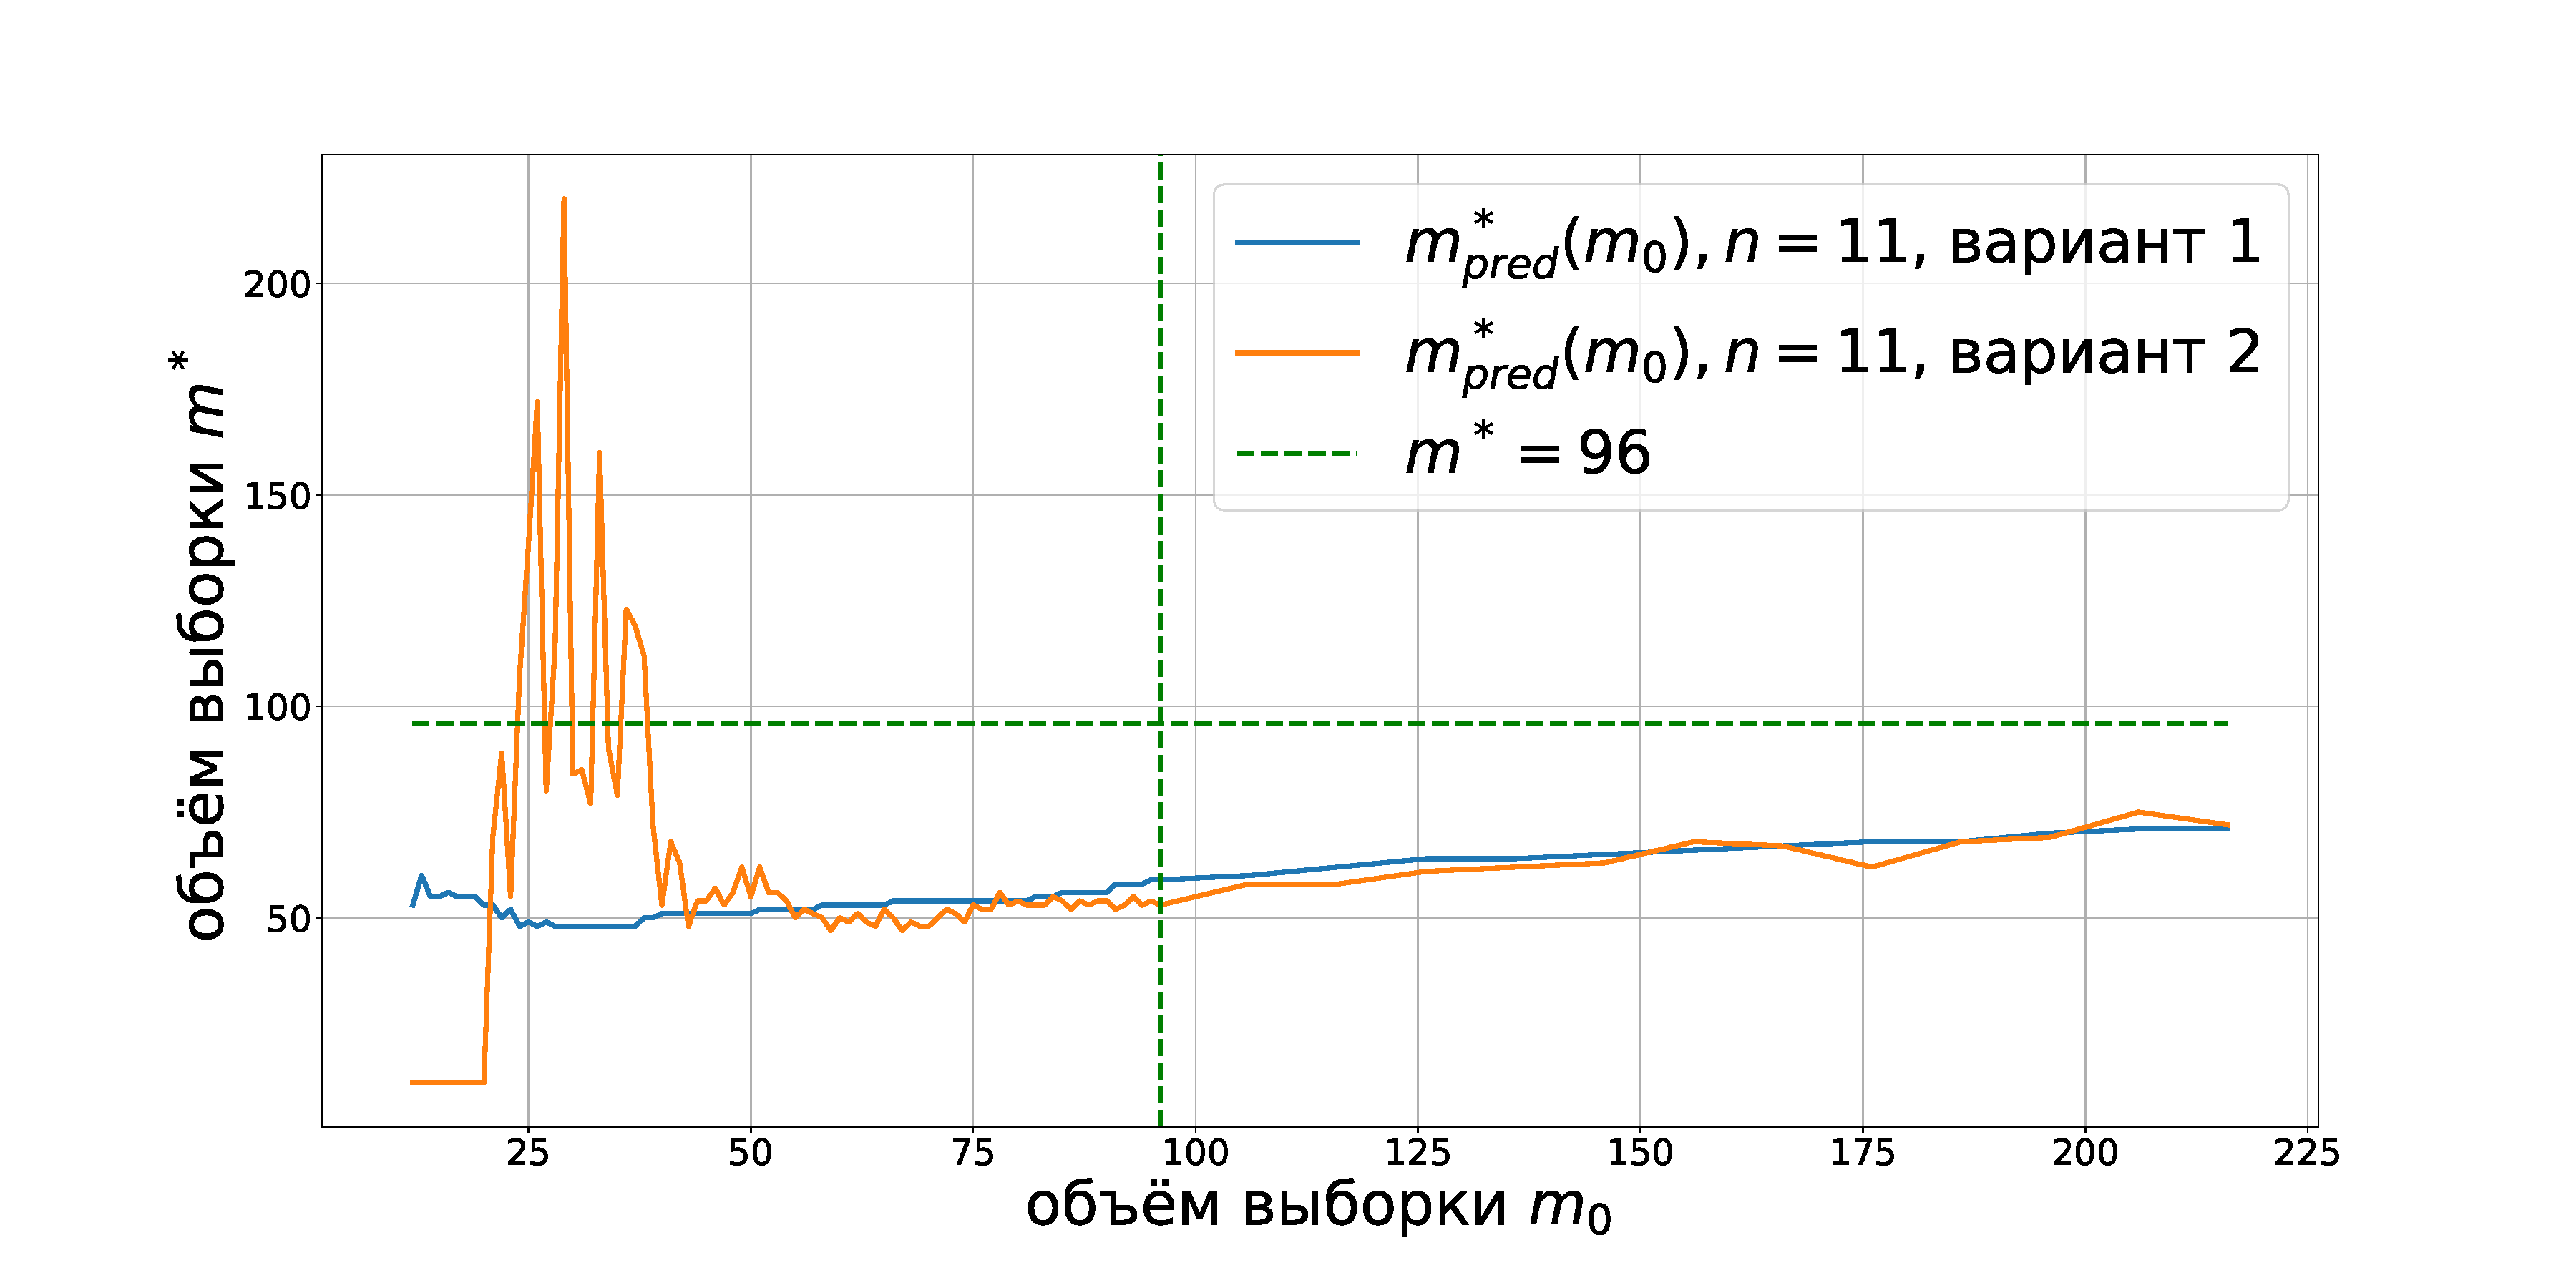
\includegraphics[width=0.5\textwidth]{../data/pics/diabetes_sample_MAPE_m_comparison_n11.pdf}}\\
\subfloat[Boston]{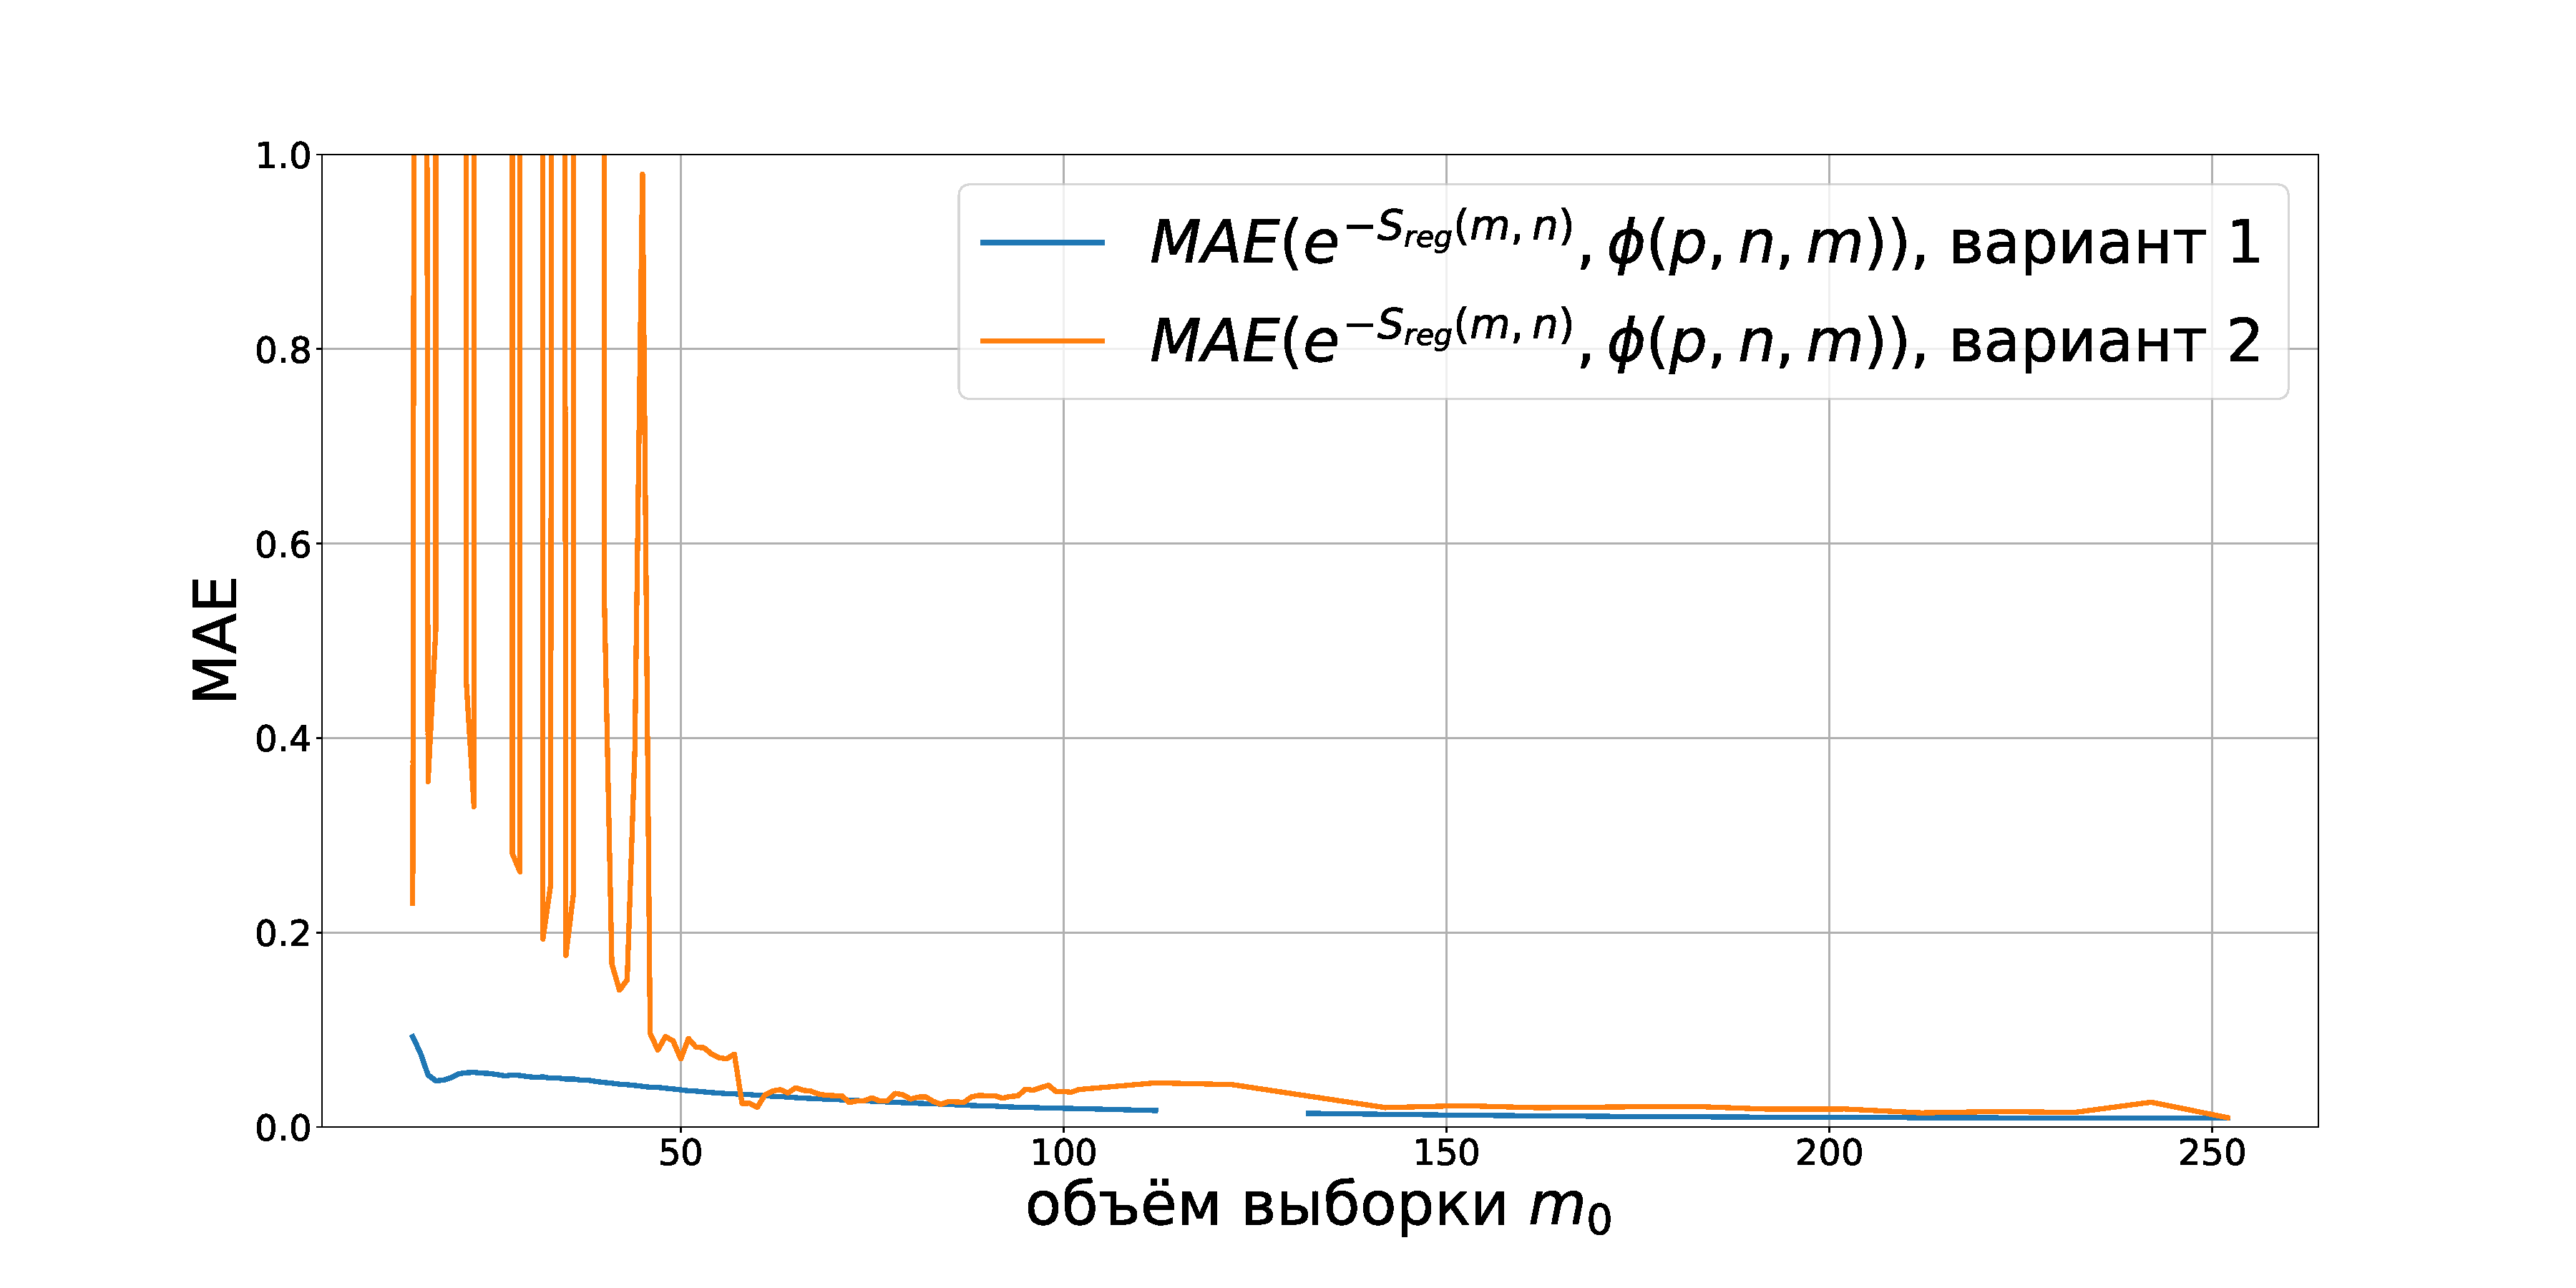
\includegraphics[width=0.5\textwidth]{../data/pics/boston_sample_MAPE_comparison.pdf}}&
\subfloat[Boston]{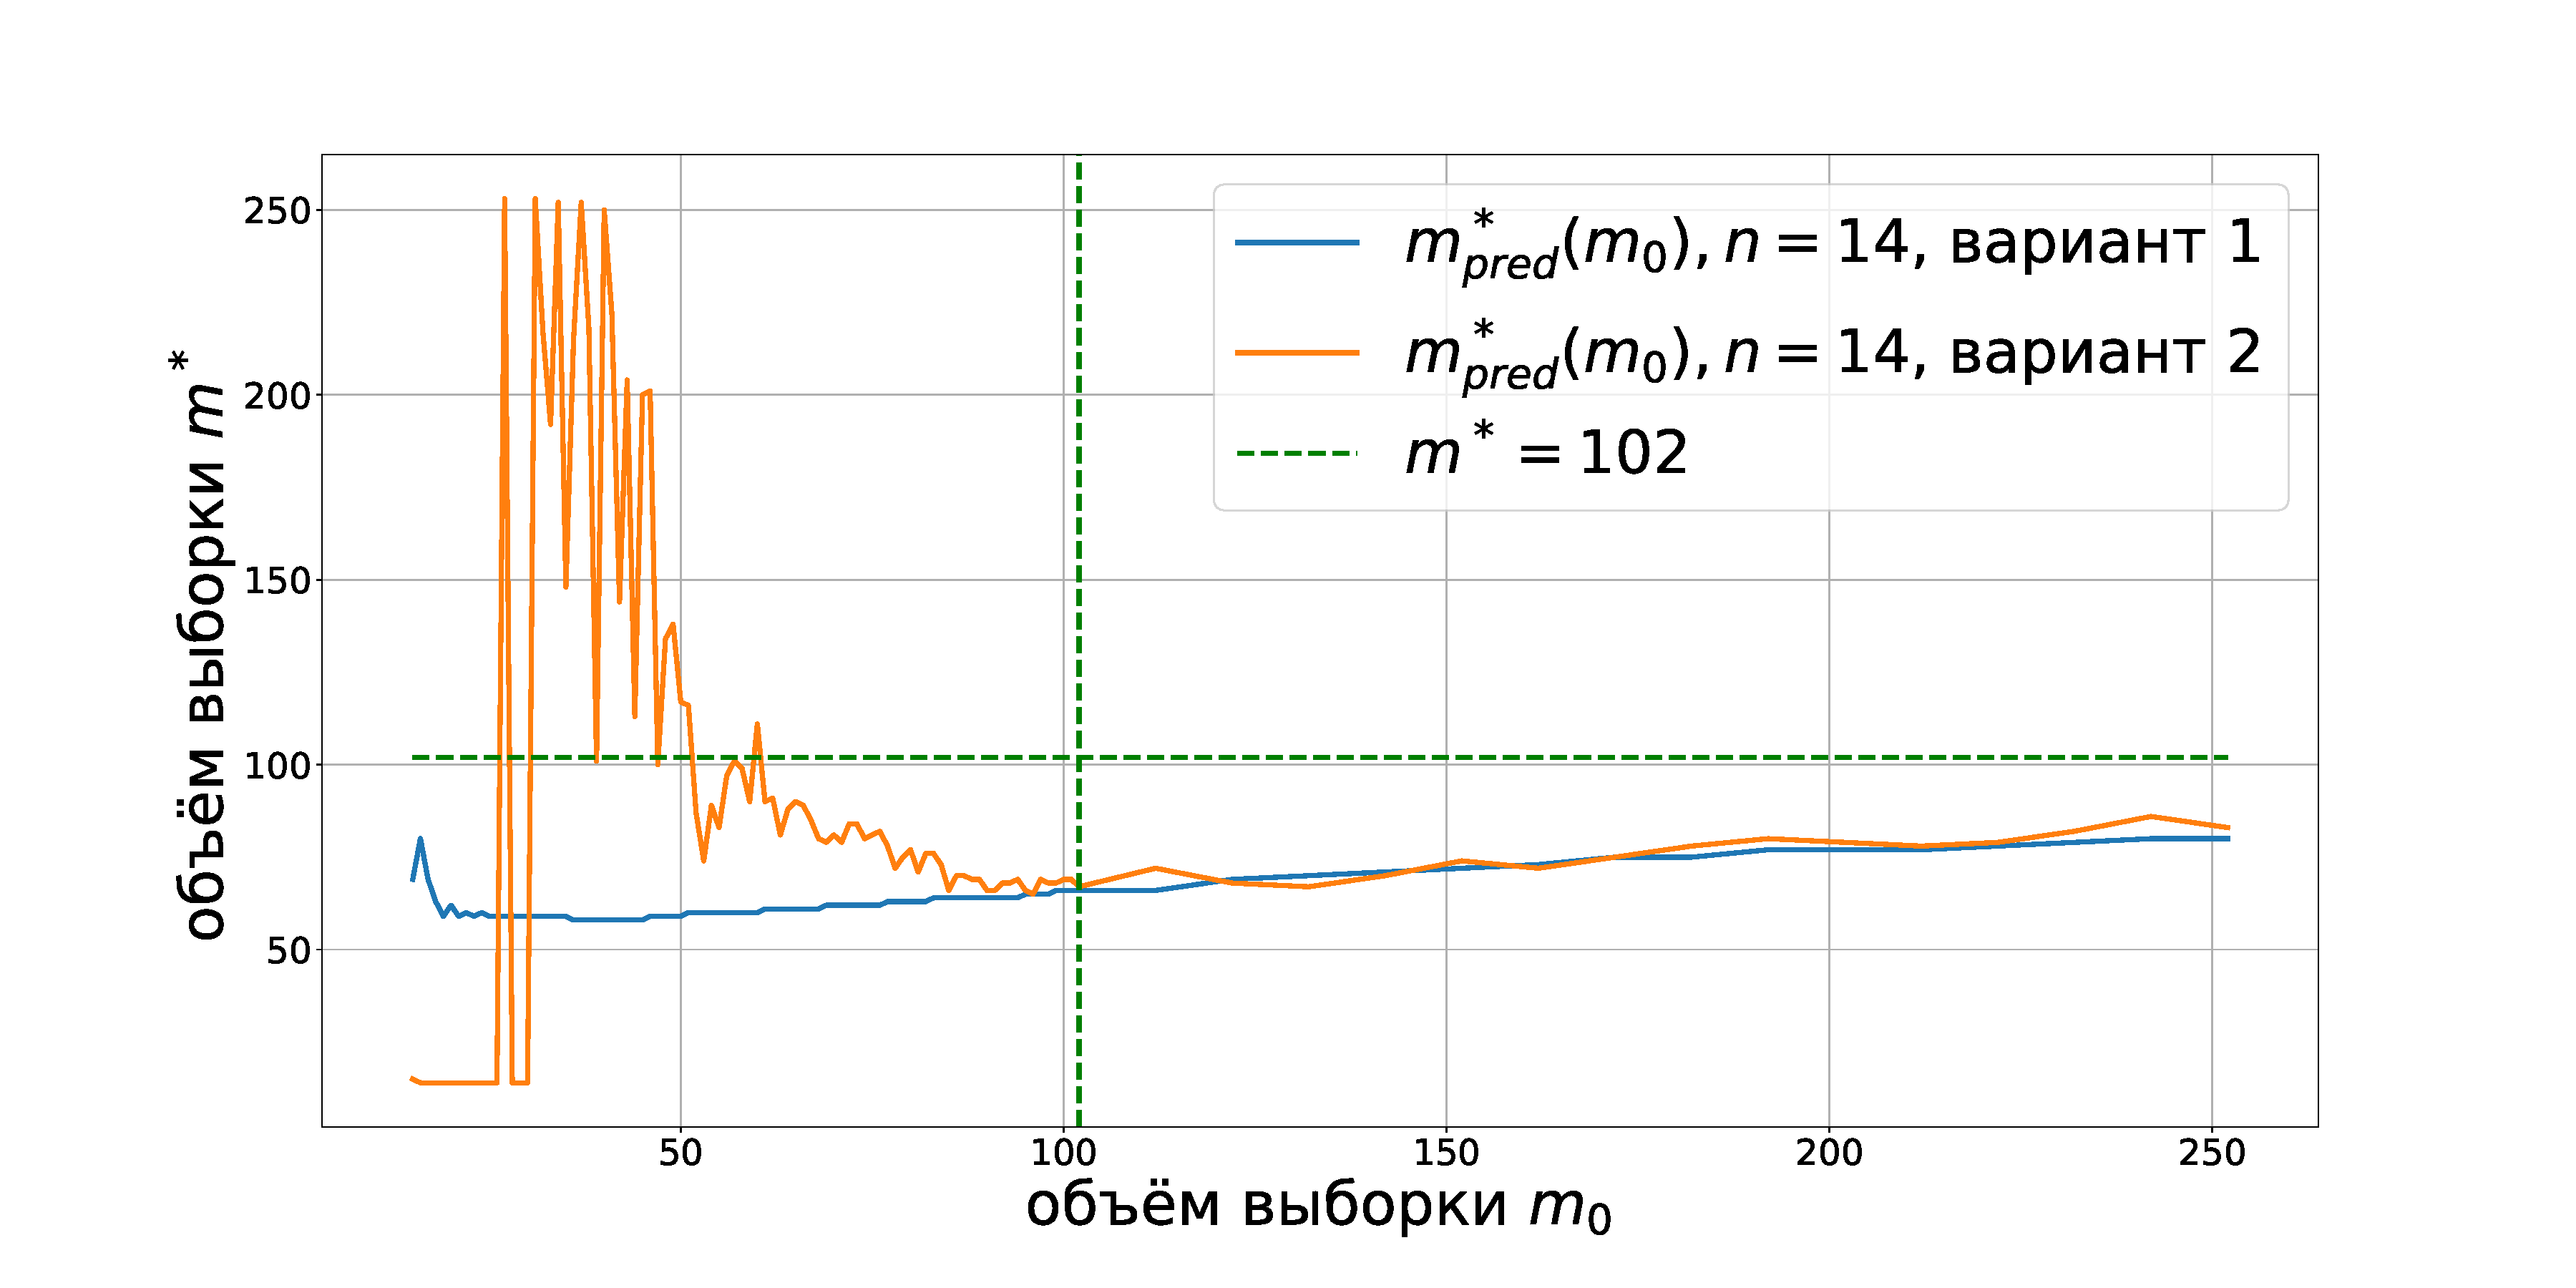
\includegraphics[width=0.5\textwidth]{../data/pics/boston_sample_MAPE_m_comparison_n14.pdf}}\\
\subfloat[Wine]{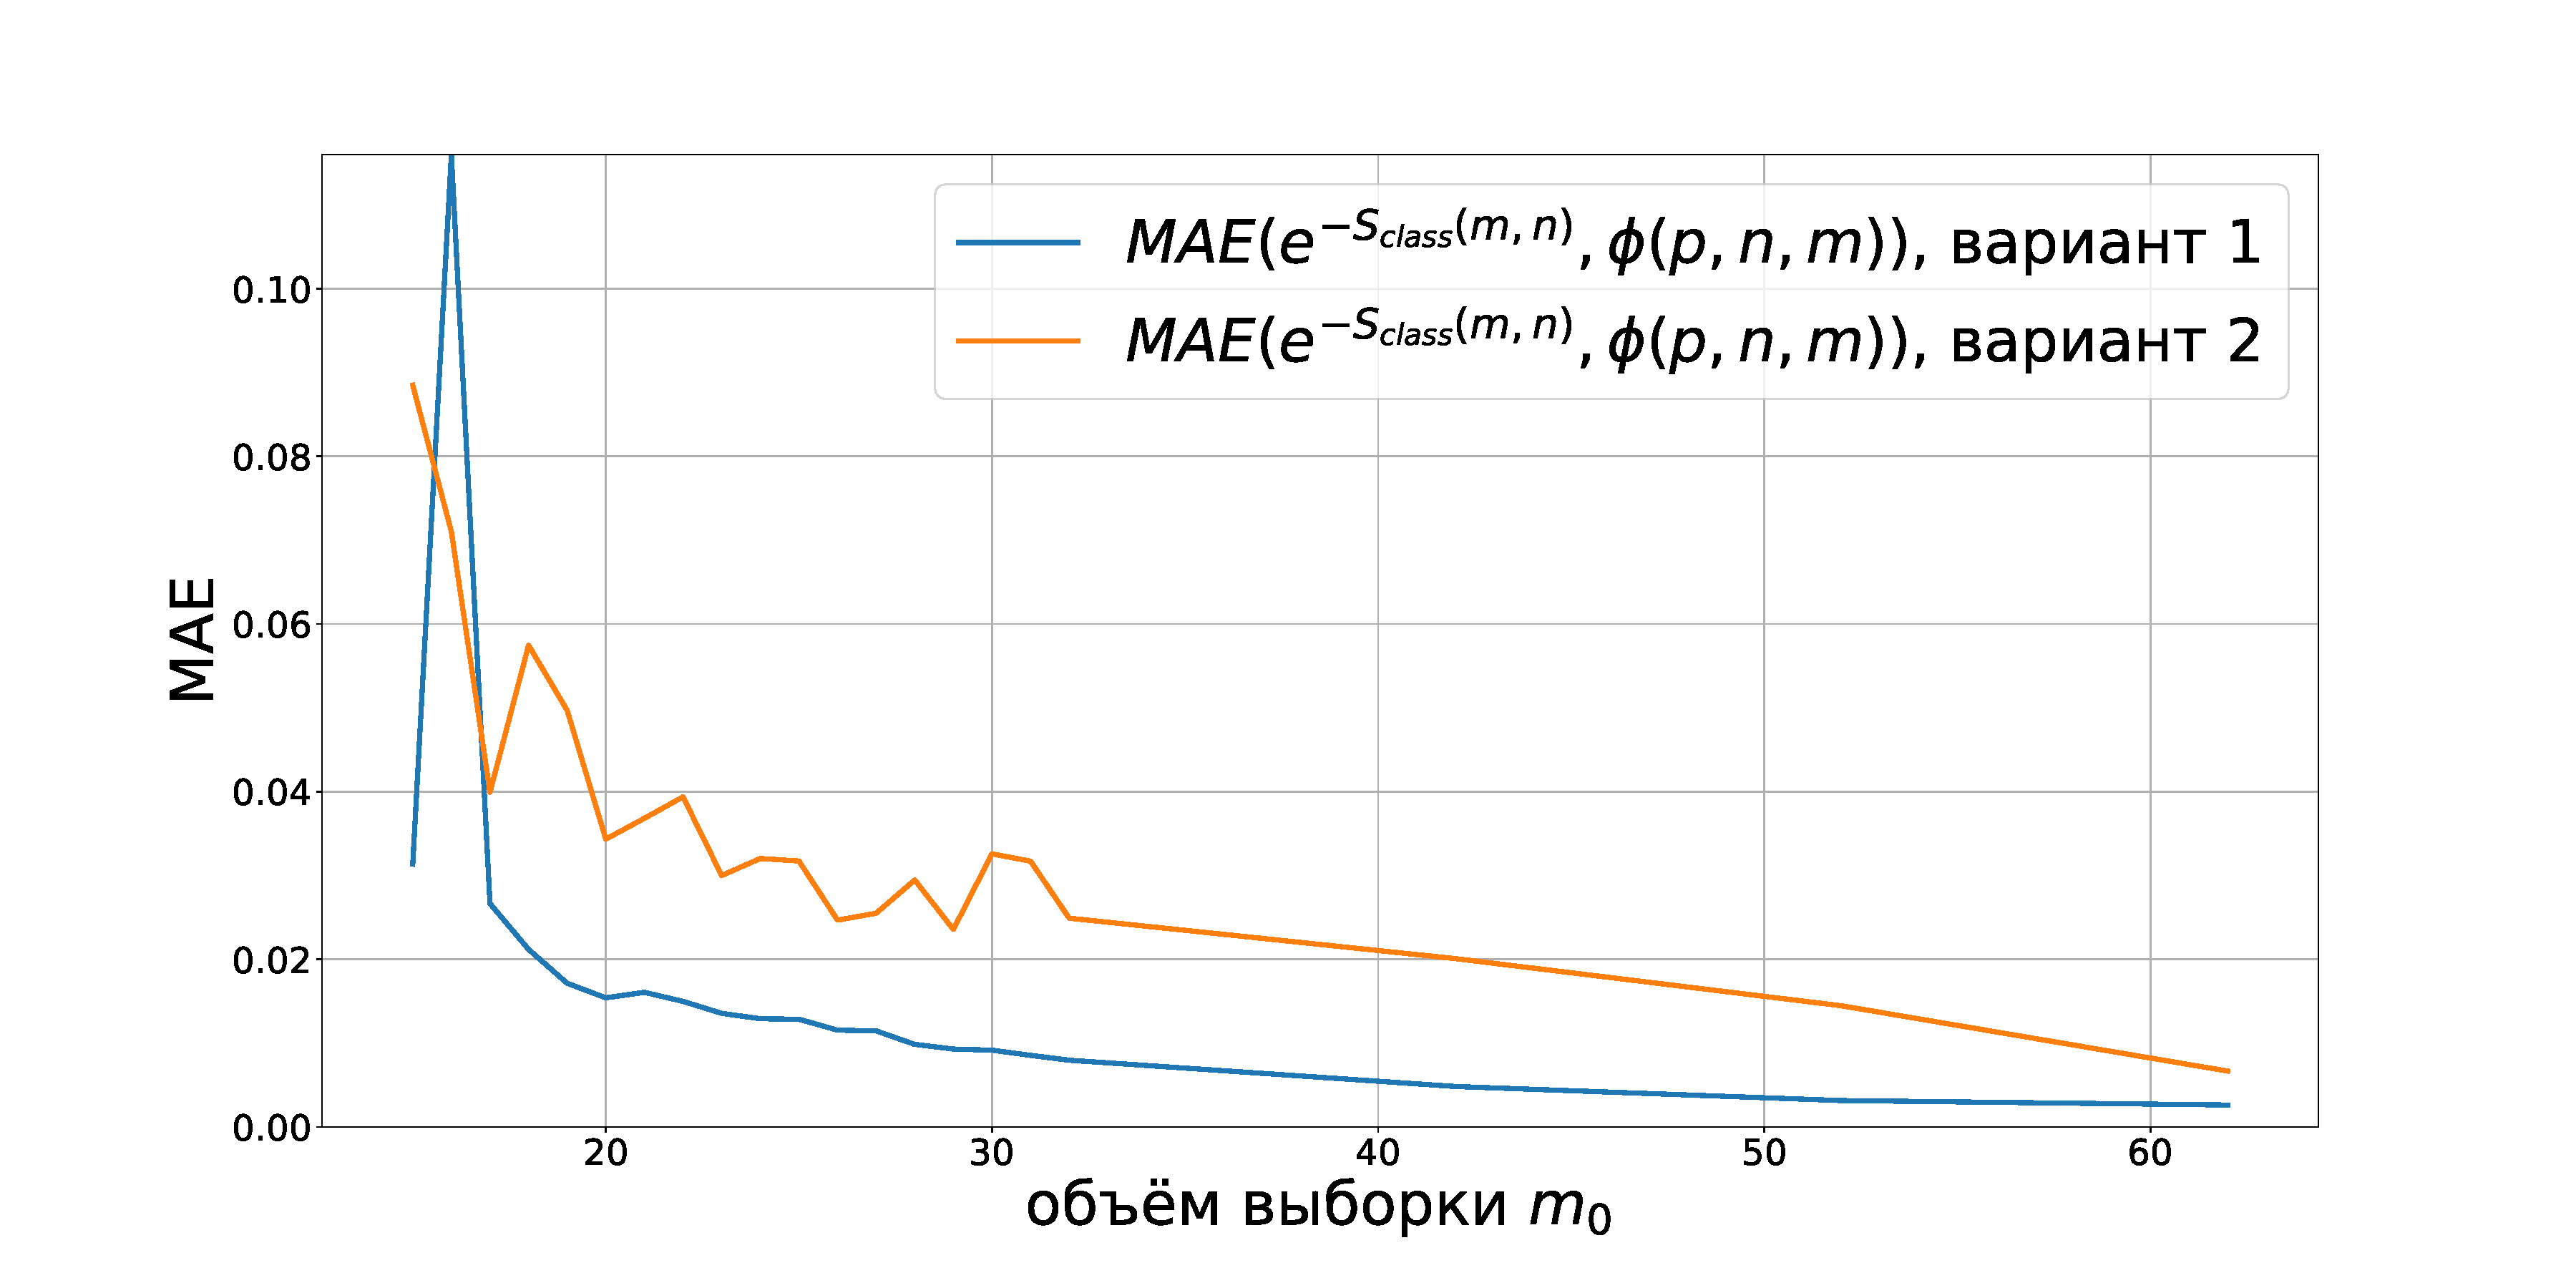
\includegraphics[width=0.5\textwidth]{../data/pics/wine_sample_MAPE_comparison.pdf}}&
\subfloat[Wine]{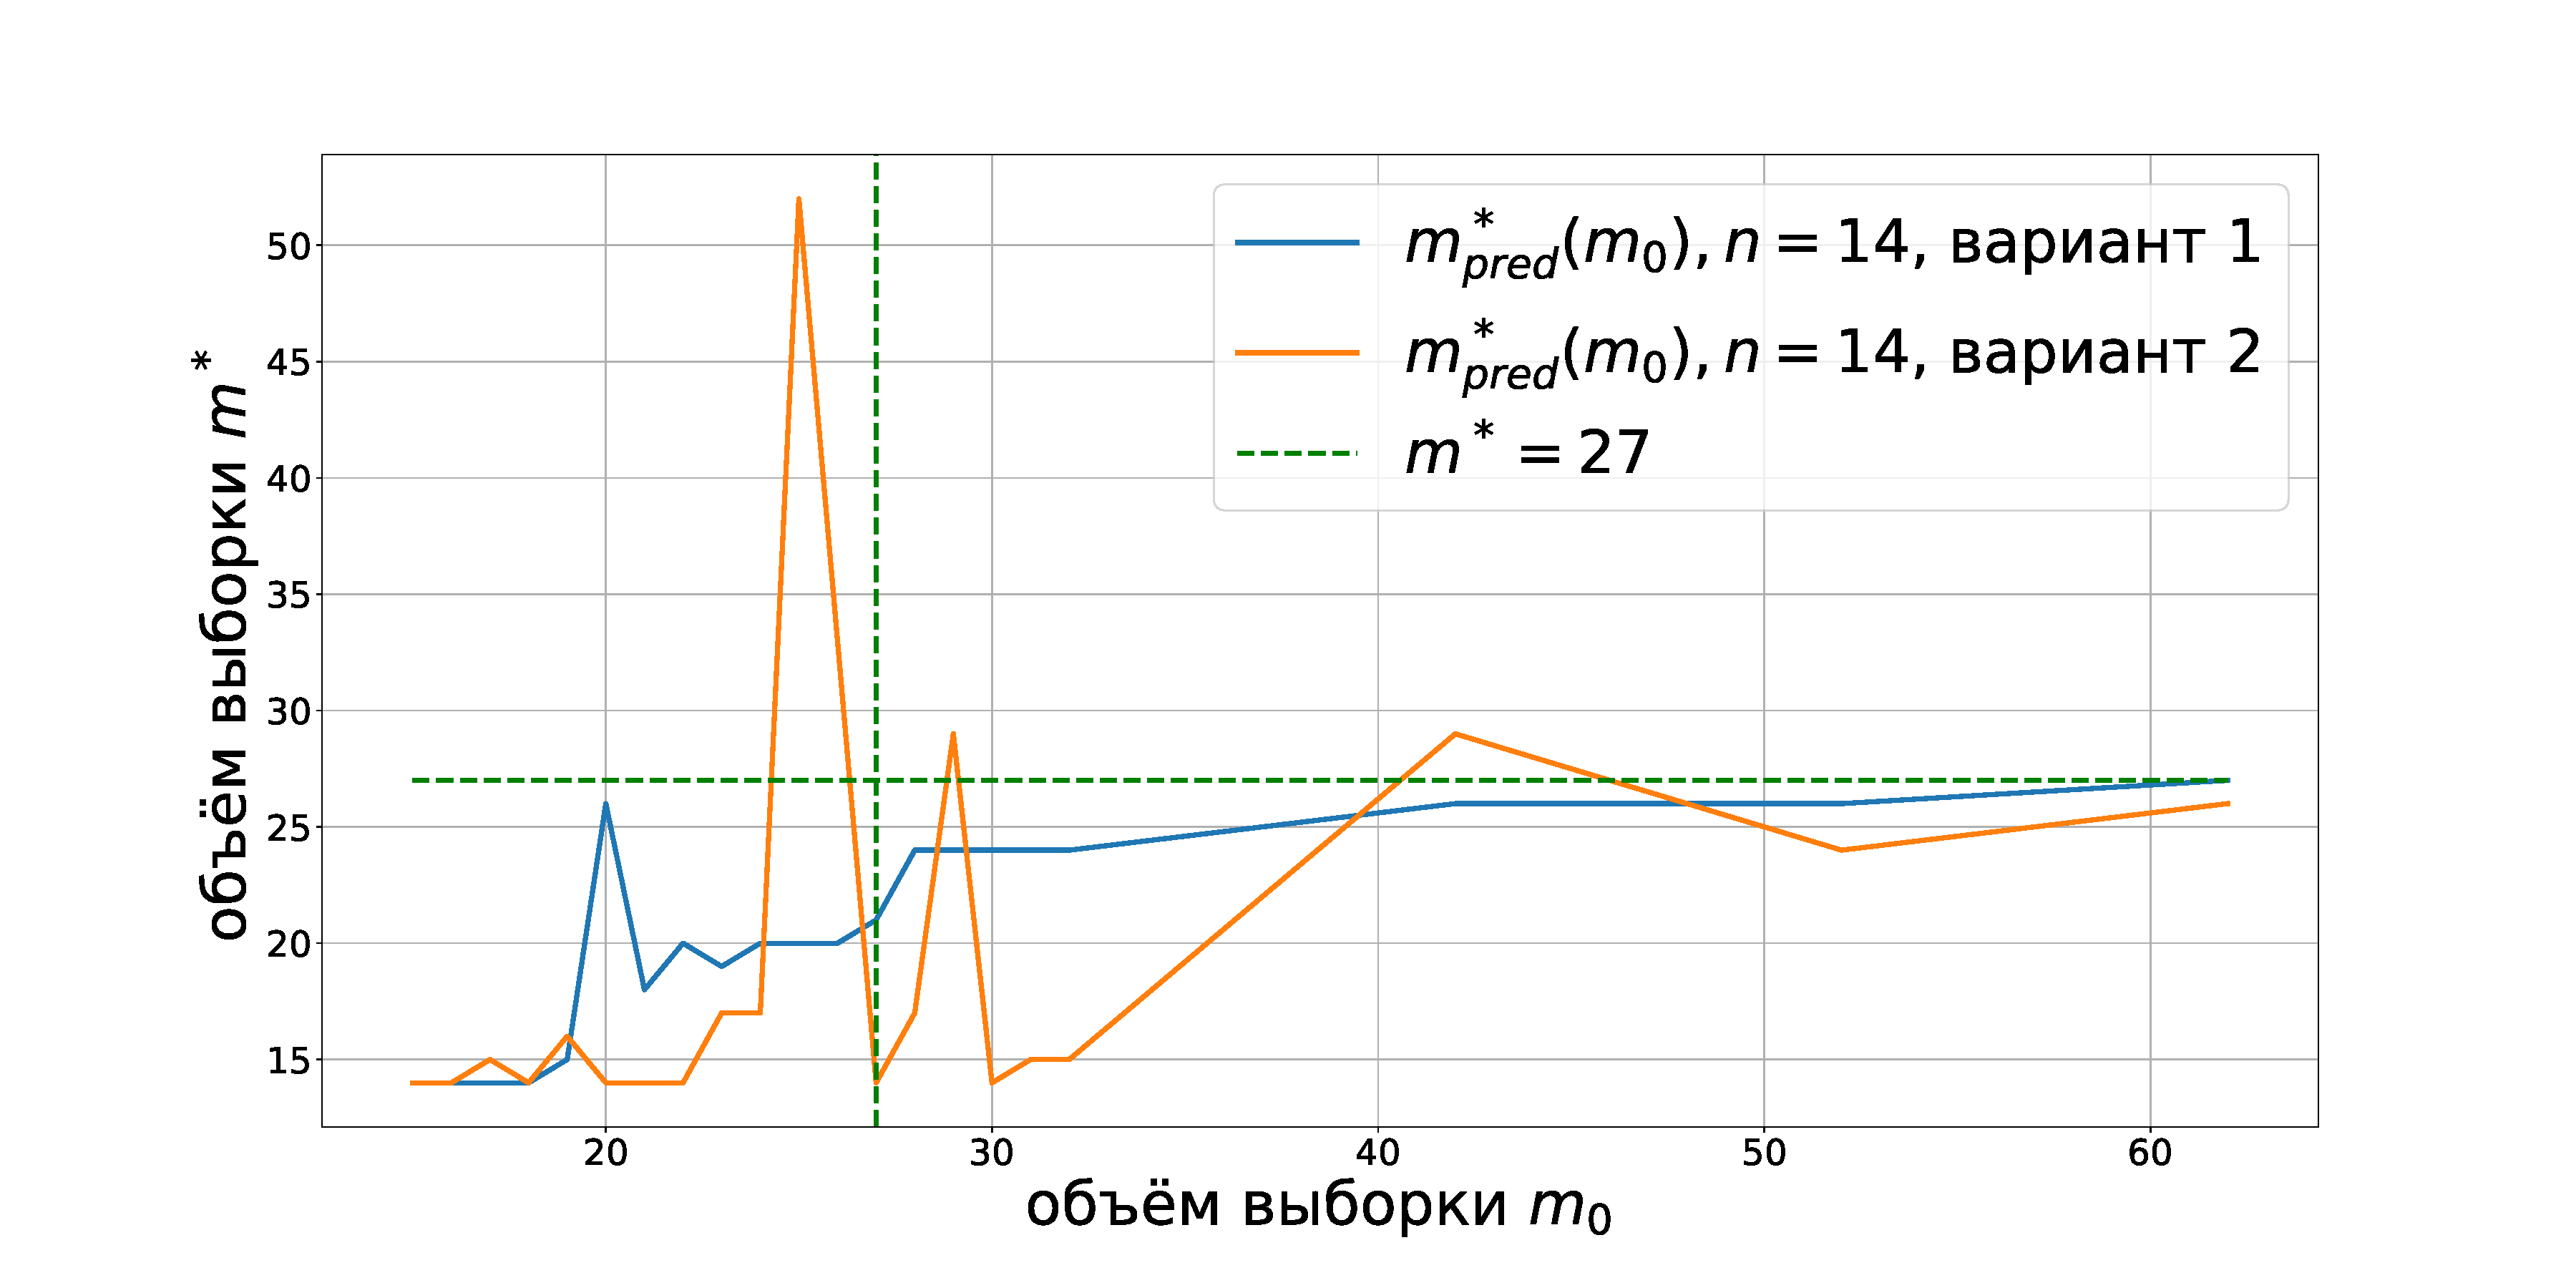
\includegraphics[width=0.5\textwidth]{../data/pics/wine_sample_MAPE_m_comparison_n14.pdf}}\\
\subfloat[Nba]{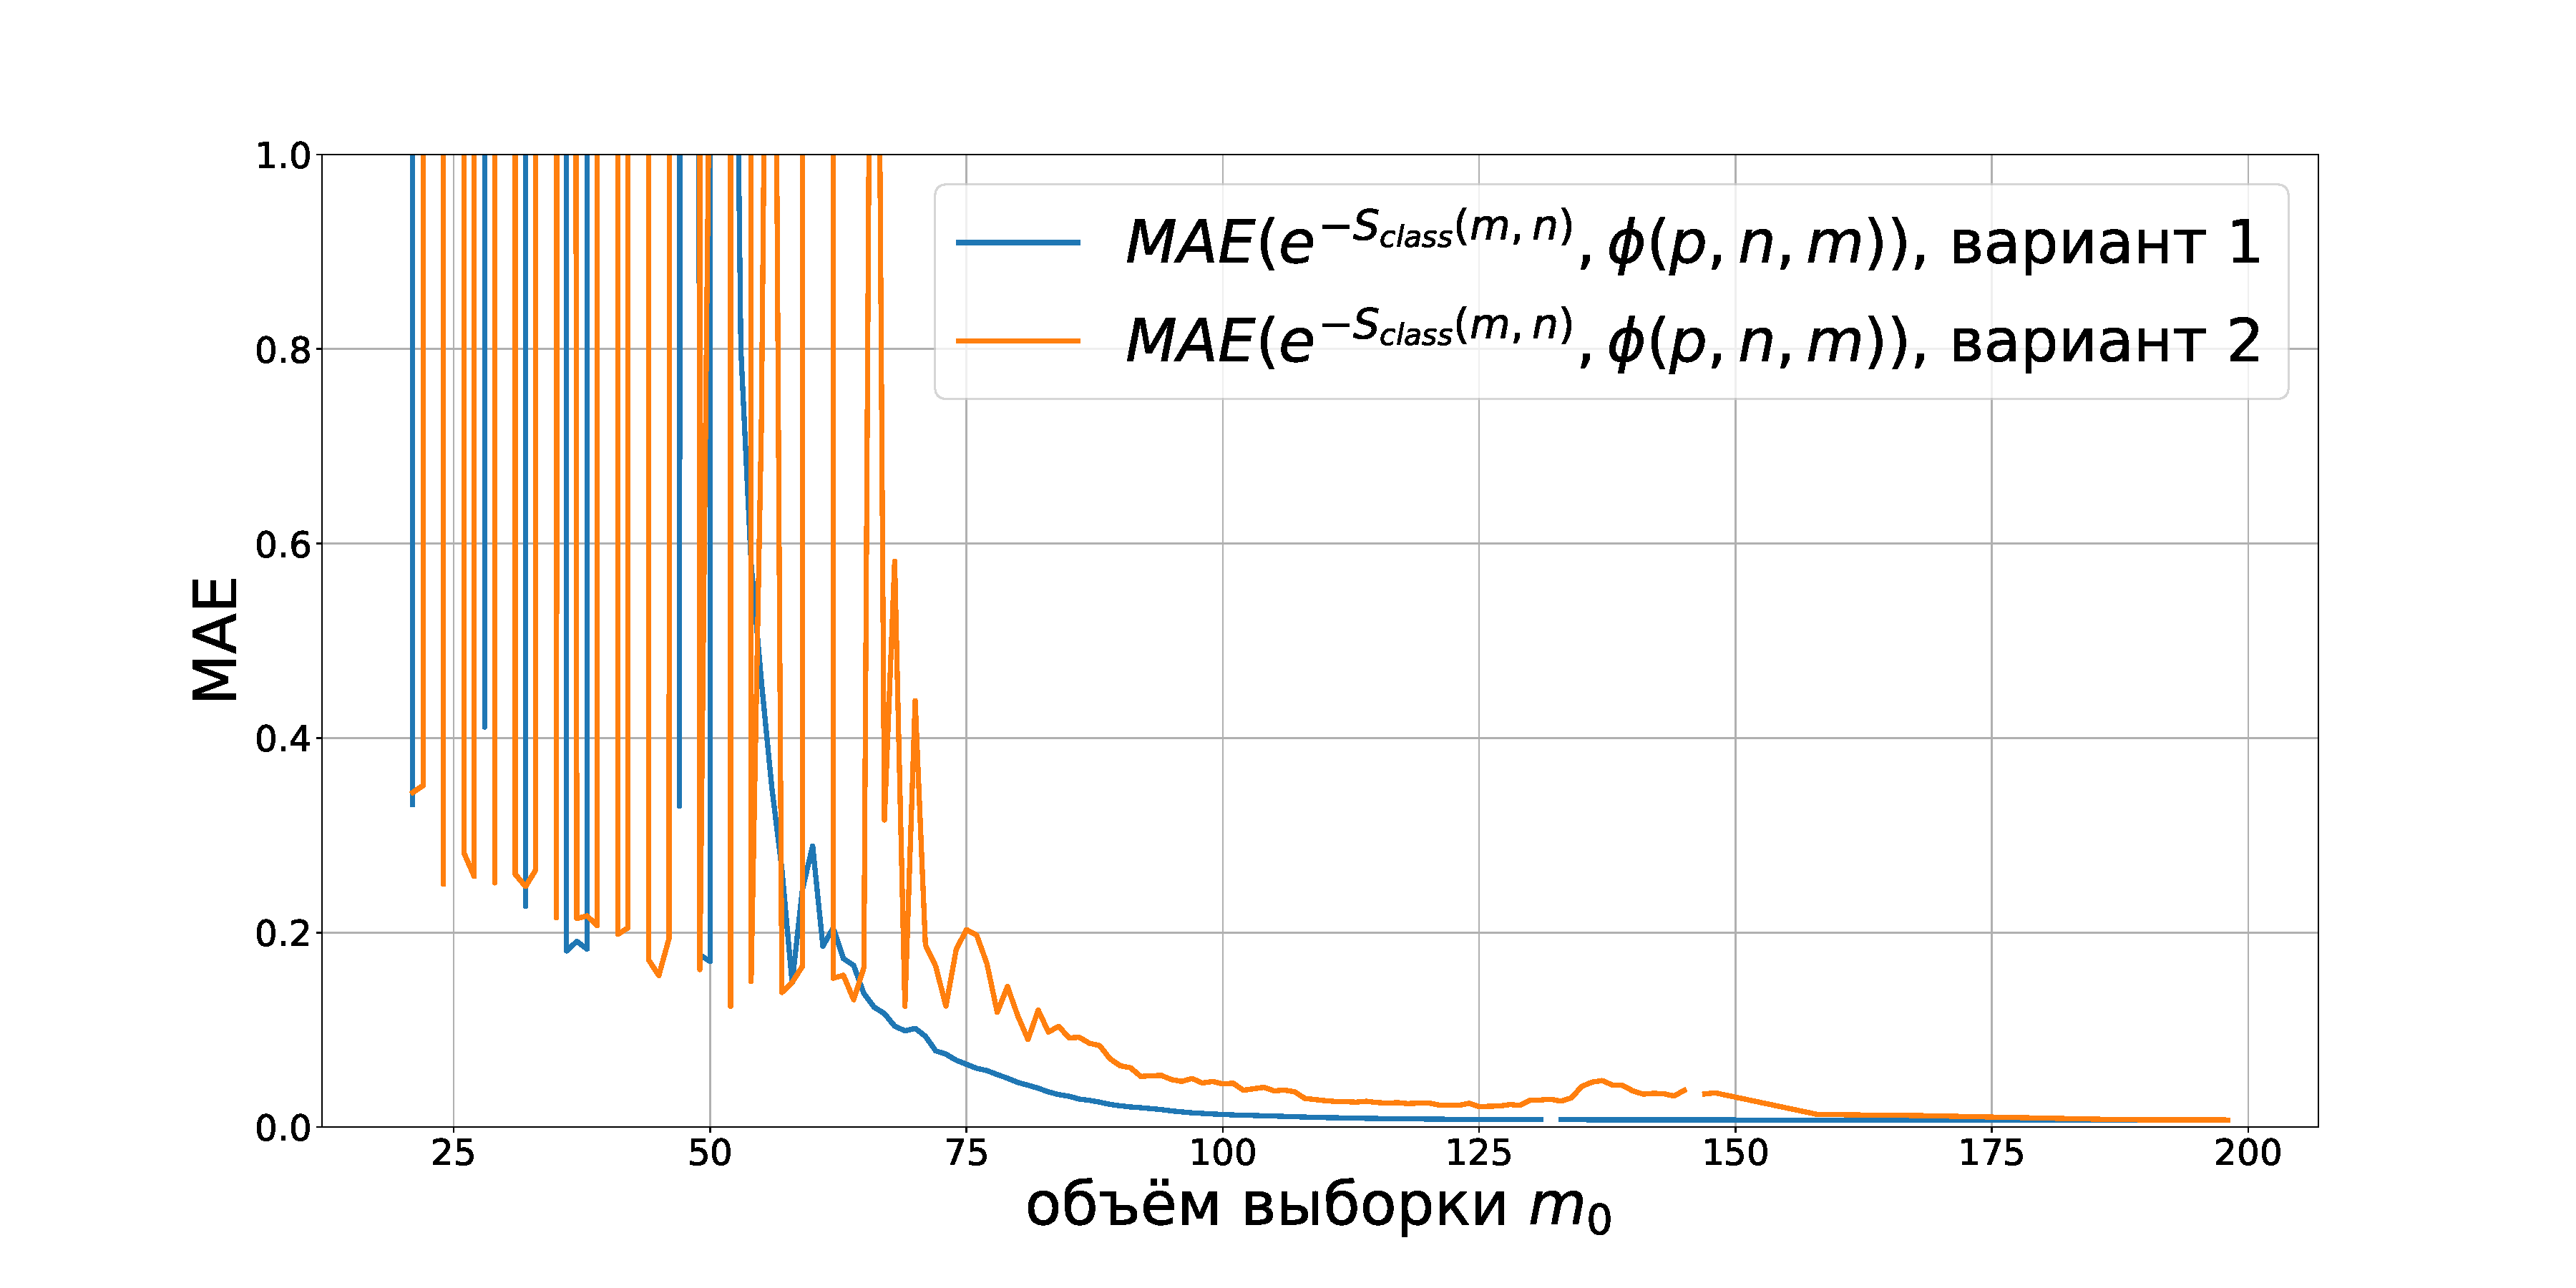
\includegraphics[width=0.5\textwidth]{../data/pics/nba_sample_MAPE_comparison.pdf}}&
\subfloat[Nba]{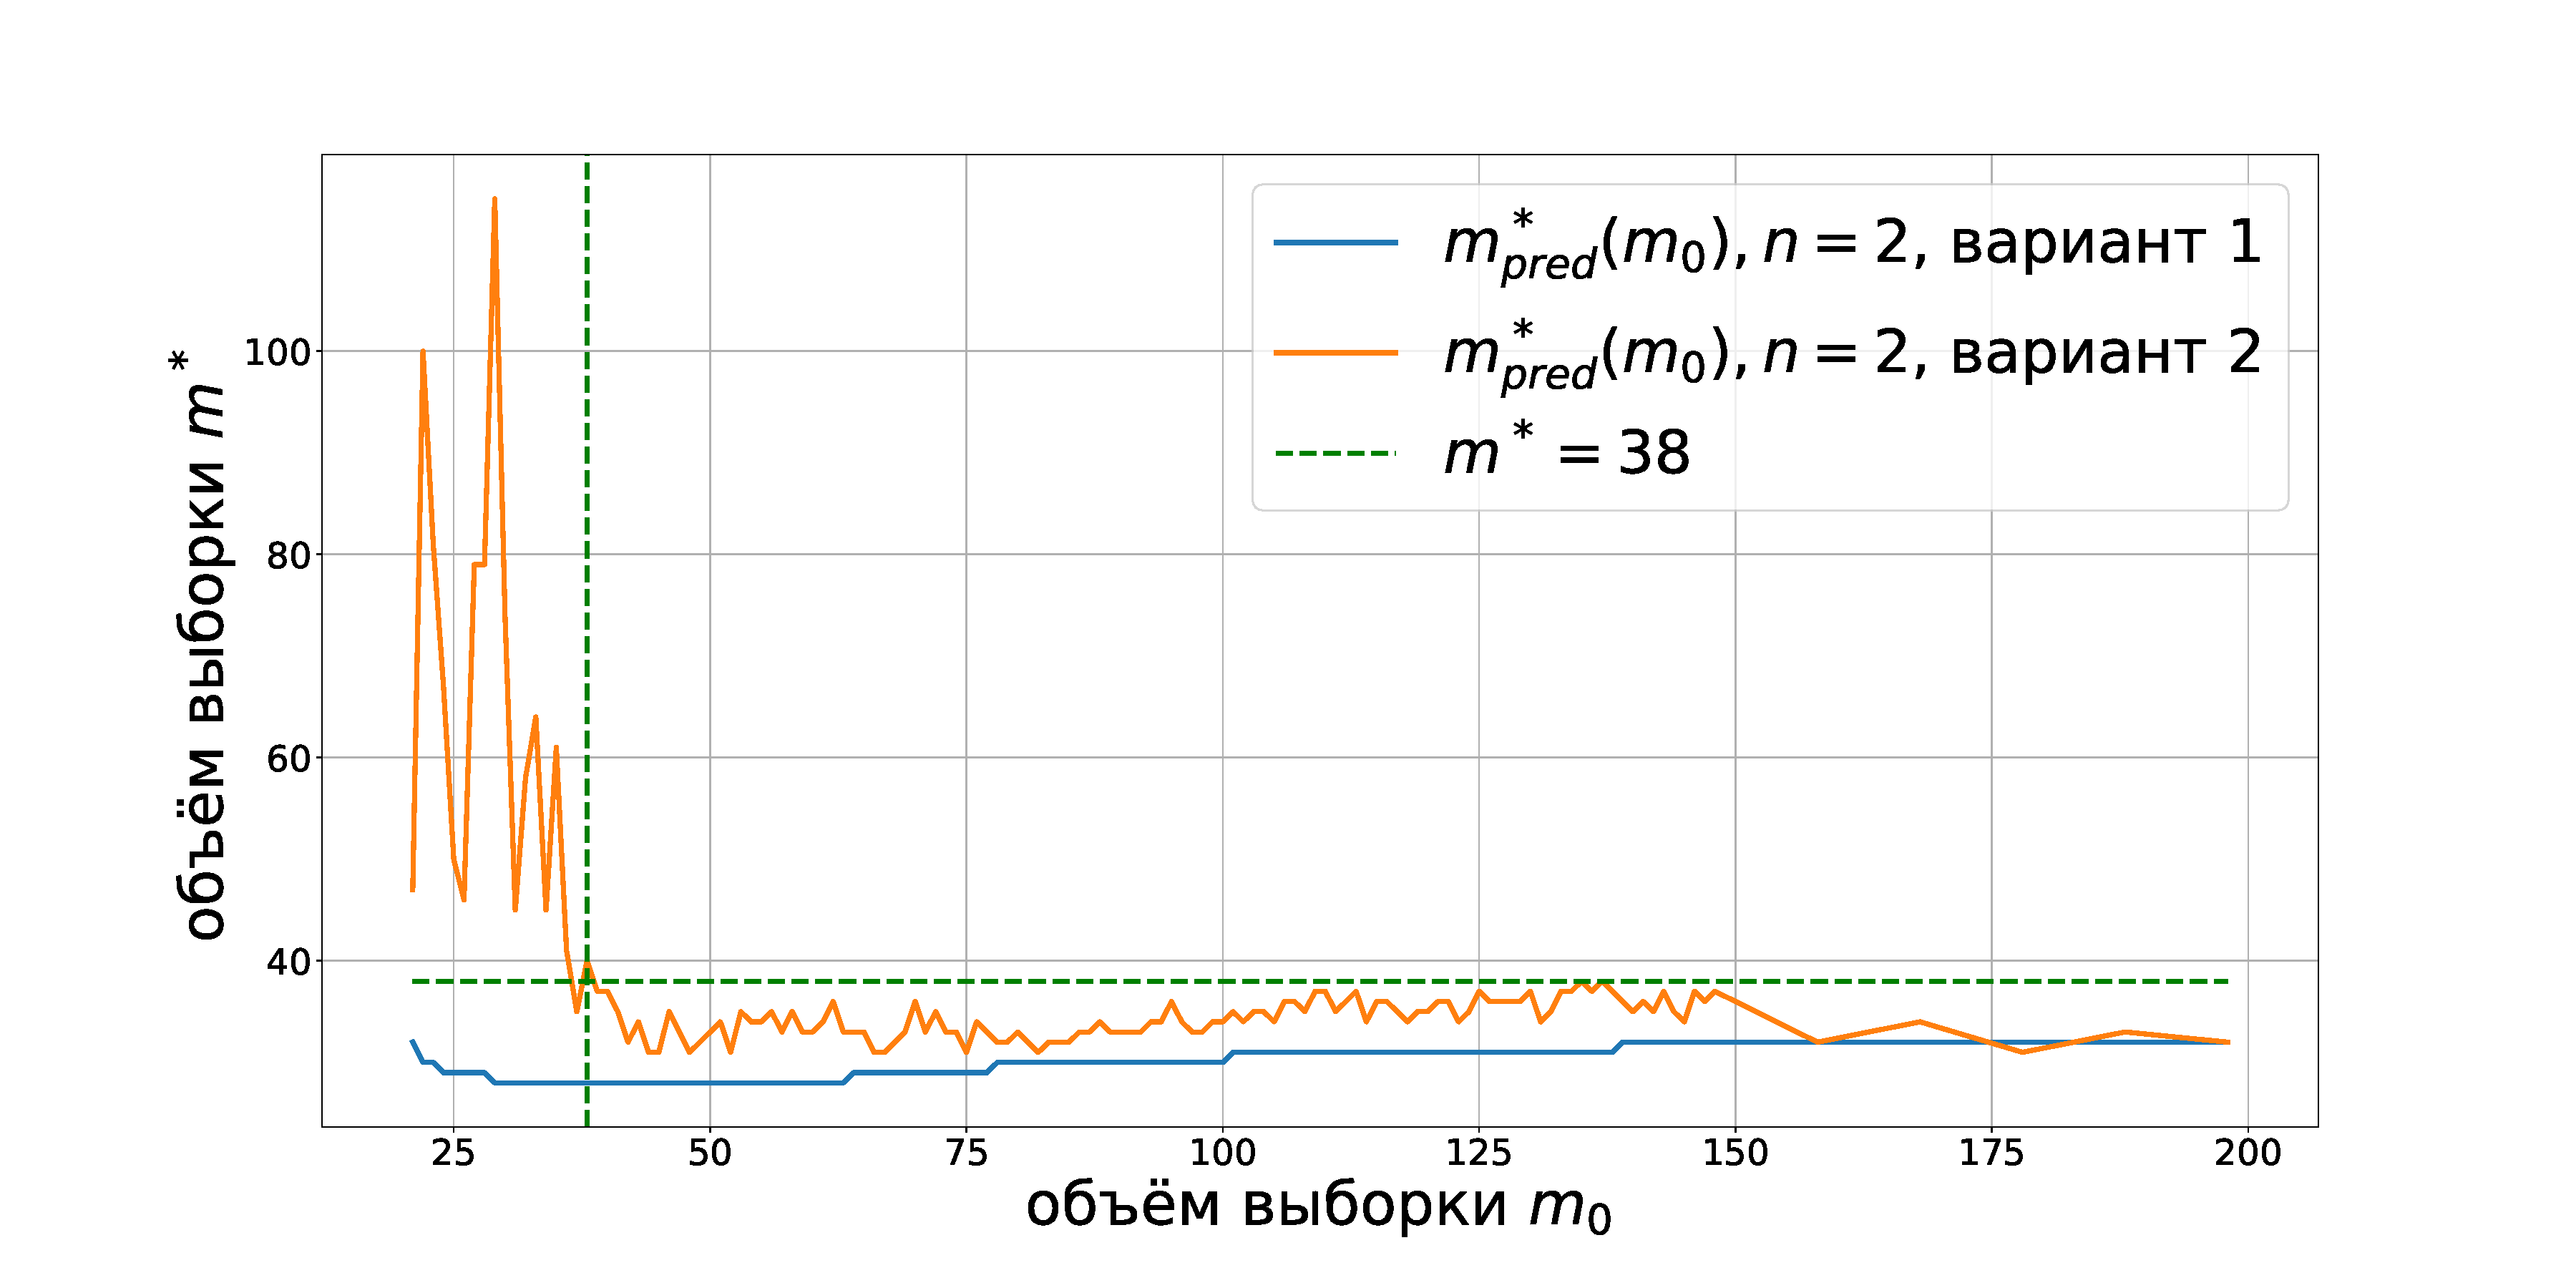
\includegraphics[width=0.5\textwidth]{../data/pics/nba_sample_MAPE_m_comparison_n2.pdf}}\\
\end{tabular}

\caption{Качество предсказания $e^{-S(m, n)}$ и $m^*$ в зависимости от объема обучающей выборки $m_0$ для выборок из UCI репозитория}
\label{fig103}
\end{figure}

\newpage
\section{Заключение}

Построен алгоритм раннего прогнозирования достаточного объёма выборки для обобщённой линейной модели. 
Для некоторых выборок задача раннего прогнозирования была успешно решена. 
Данный алгоритм можно улучшить путём использования в построении модели аппроксимации $\phi(m) \sim \hat{l}(m)$ свойств оценки вектора параметров $\hat{\mathbf{w}}$ обобщенной линейной модели.

\newpage
\begin{thebibliography}{1}

\bibitem{Self-Mauritsen-1998}
S.\,G.\;Self and R.\,H.\;Mauritsen Power/sample size calculations for generalized linear
models ~// Biometrics, 1988. Vol. 44. P. 79-86. 

\bibitem{Shieh-2000}
G.\,Shieh On power and sample size calculations for likelihood ratio tests in generalized
linear models~// Biometrics, 2000. Vol. 56. P. 1192-1196.

\bibitem{Shieh-2005}
G.\,Shieh On power and sample size calculations for Wald tests in generalized linear
models~// Journal of Statistical Planning and Inference, 2005. Vol. 128. P. 43-59.


\bibitem{Wang-Gelfand-2002}
Fei Wang and Alan E. Gelfand A Simulation-based Approach to Bayesian Sample Size
Determination for Performance under a Given Model and for Separating Models ~// Statistical Science, 2002. Vol. 17. P. 193-208.

\bibitem{Figueroa-2012}
Rosa L Figueroa, Qing Zeng-Treitler, Sasikiran Kandula and Long H Ngo Predicting sample size required for classification
performance ~// BMC Medical Informatics and Decision Making.

\bibitem{Dobbin-2008}
Kevin K. Dobbin,Yingdong Zhao, and Richard M. Simon How Large a Training Set is Needed to Develop a Classifier for Microarray Data? ~// American Association for Cancer Research, 2008.

\end{thebibliography}

\end{document}


